\documentclass[draft]{book}
\usepackage[utf8]{inputenc}
\usepackage[italian]{babel}
\usepackage{csquotes}
\usepackage[a4paper, bottom=4cm]{geometry}
\usepackage{graphicx}
\usepackage[hidelinks]{hyperref}
\usepackage{listings}
\usepackage{xcolor}
\usepackage{inconsolata}
\usepackage{minted}
\usepackage{tcolorbox}
\tcbuselibrary{minted,skins}
\usepackage{charter}
\usepackage[Lenny]{fncychap}
\usepackage{fancyhdr}
\ChTitleVar{\Huge\sc}
\usepackage{caption}
\usepackage[cleardoublepage=plain]{scrextend}

% To clear page numbers from footer, and header line at the start of every chapter
\fancypagestyle{plain}{\fancyhf{}\renewcommand{\headrulewidth}{0pt}}
\pagestyle{fancy}
\fancyhf{}% Clear header/footer
\fancyhead[RE]{\nouppercase\leftmark}
\fancyhead[LO]{\nouppercase\rightmark}
\fancyhead[LE,RO]{\thepage}

\let\OldTexttt\texttt
\renewcommand{\texttt}[1]{\textcolor{teal}{\OldTexttt{#1}}}

% Ridefinisci il formato della didascalia
\DeclareCaptionFormat{custom}{\textbf{#1#2}#3} % Grassetto per "Figura 3.1"
\captionsetup[figure]{format=custom} % Applica il formato alle figure

\usepackage[style=alphabetic]{biblatex}
\addbibresource{sources.bib}

\definecolor{sol-background}{HTML}{FDF6E3}
\definecolor{sol-text}{HTML}{657B83}
\definecolor{sol-comments}{HTML}{93A1A1}
\definecolor{sol-keywords}{HTML}{859900}
\definecolor{sol-strings}{HTML}{2AA198}
\definecolor{sol-constants}{HTML}{268BD2}
\definecolor{sol-functions}{HTML}{B58900}

\definecolor{one-background}{HTML}{FAFAFA}
\definecolor{one-text}{HTML}{383A42}
\definecolor{one-comments}{HTML}{A0A1A7}
\definecolor{one-keywords}{HTML}{A626A4}
\definecolor{one-strings}{HTML}{50A14F}
\definecolor{one-constants}{HTML}{986801}
\definecolor{one-functions}{HTML}{4078F2}

\renewcommand\lstlistingname{Codice}
\renewcommand\lstlistlistingname{Elenco dei frammenti di codice}

\newtcblisting{pycode}[1][]{
  listing engine=minted,
  colback=teal!6,
  colframe=black!70,
  listing only,
  minted style=tango,
  minted language=Python,
  minted options={breaklines=true,escapeinside=||,linenos=true,numbersep=3mm,texcl=true,#1},
  left=5mm,enhanced,
  overlay={\begin{tcbclipinterior}\fill[teal!4] (frame.south west)
            rectangle ([xshift=5mm]frame.north west);\end{tcbclipinterior}},
  frame hidden,
}
\newtcblisting{jscode}[1][]{
  listing engine=minted,
  colback=sol-background!50,
  colframe=black!70,
  listing only,
  minted style=solarized-light,
  minted language=TypeScript,
  minted options={breaklines=true,escapeinside=||,linenos=true,numbersep=3mm,texcl=true,#1},
  left=5mm,enhanced,
  overlay={\begin{tcbclipinterior}\fill[sol-background!30] (frame.south west)
            rectangle ([xshift=5mm]frame.north west);\end{tcbclipinterior}},
  frame hidden,
}
\newtcblisting{vuesfc}[1][]{
  listing engine=minted,
  colback=green!5,
  colframe=black!70,
  listing only,
  minted style=perldoc,
  minted language=html,
  minted options={breaklines=true,escapeinside=||,linenos=true,numbersep=3mm,texcl=true,#1},
  left=5mm,enhanced,
  overlay={\begin{tcbclipinterior}\fill[green!2] (frame.south west)
            rectangle ([xshift=5mm]frame.north west);\end{tcbclipinterior}},
  frame hidden,
}

\begin{document}
  \newgeometry{top=4cm,bottom=4cm,left=2cm,right=2cm}
\begin{titlepage}
    \begin{center}
        \vspace{4cm}
        \begin{figure}[!h]
            \centering
            
\includegraphics{img/unibs.png}
        \end{figure}
        {\Large{\textsc{Dipartimento di \textbf{Ingegneria dell'Informazione}}}\par}
        \vspace{2mm}
        {\large \centering{\textsc{Corso di laurea in \textbf{Ingegneria Informatica}}}\par}
    \end{center}

    \vspace{35mm}
 
    \begin{center}
        {\huge {\bf TESI DI LAUREA MAGISTRALE}\par}
        \vspace{5mm}
        {\LARGE \bfseries Progettazione e sviluppo di un'applicazione web multi-tenant per il vulnerability assessment}
    \end{center}
 
    \vspace{40mm}

    \noindent
        {\large{\bf Relatore:} Prof. Francesco Gringoli} \\
        \vspace{5mm}
        \begin{flushright}
            {\large{\bf Laureando:} Ivan Ravasi} \\
            \vspace{2mm}
            {\large{\bf Matricola:} 727294}
        \end{flushright}
    \hfill
    \newline
    \vspace{5mm}
 
    \vfill
    \begin{center}
        {\large Anno Accademico 2024 / 2025}
    \end{center}
\end{titlepage}
\restoregeometry
  \tableofcontents
  \listoffigures
  \chapter{Introduzione}
  \section{Contesto}
Oggigiorno l'informatica e le reti di telecomunicazione sono diventate delle parti integranti e pervasive nelle nostre vite. Senza che ce ne accorgiamo, dispositivi di ogni genere e reti di ogni dimensione sono arrivati a diventare parte integrante del quotidiano.

Per questo motivo, garantire la loro sicurezza diventa ogni giorno sempre più importante. Infatti, ogni singolo nodo di rete, anche quello più insignificante, nelle mani del giusto attaccante può diventare inestimabile sia in sé che come eventuale testa di ponte per un attacco più esteso e massiccio.

Tutti questi rischi valgono per chiunque disponga di servizi esposti in rete, indipendentemente dalla loro popolarità. Infatti, la rete è oramai periodicamente scandita metodicamente da attaccanti che cercano con strumenti automatici qualunque tipo di servizio dotato di vulnerabilità note, così da assicurarsi un facile bottino. Inutile dire che la necessità di un controllo di sicurezza possa diventare solamente ancora più critica per grandi aziende ed entità maggiormente esposte in rete.

Per tutti questi motivi è buona norma verificare regolarmente la sicurezza della propria rete e dei propri servizi esposti in Internet.

\section{Verifica della sicurezza di un nodo di rete}
La sicurezza dei propri nodi di rete può essere verificata tramite delle procedure genericamente dette di \textbf{vulnerability assessment} (lett. \emph{verifica delle vulnerabilità}). L'obiettivo di queste procedure è:
\begin{itemize}
    \item Controllare se i servizi visibili dalla rete contengono delle vulnerabilità software.
    \item Verificare se queste vulnerabilità corrispondono a rischi di sicurezza noti.
    \item Classificarle e valutarne il grado di rischio, così da indurre una gerarchia di priorità.
\end{itemize}

\subsection{Strumenti disponibili}
Esistono molte modalità con cui queste procedure possono essere eseguite, più o meno manuali. Tuttavia, in ambito di produzione e non solo è regolare l'uso di \textbf{vulnerability scanner}, applicativi dedicati allo scopo e che a fronte di una lista di \emph{host} di rete ne verifica la sicurezza, comparando le vulnerabilità riscontrate con dei \emph{database} costantemente aggiornati di vulnerabilità note.

Esistono molti scanner di questo tipo, a pagamento e non, con vari tipi di licenze, specifiche e requisiti, ma in generale tutti svolgono lo stesso compito: verificare le vulnerabilità reperite in fase di scansione confrontandole con database noti. I principali fattori di differenza sono il costo e le funzionalità ulteriori fornite in assistenza all'utente: reportistica avanzata, suggerimento di soluzioni, correzioni automatiche delle vulnerabilità fornite, verifiche aggiuntive o euristiche, o altro ancora.

\section{Casi d'uso}
Come già detto, la sicurezza della propria presenza in rete dovrebbe essere curata da chiunque, indipendentemente dalle proprie esigenze.

Tuttavia, l'installazione e la configurazione degli scanner sopracitati spesso è fuori dalle possibilità per la maggior parte dei soggetti interessati, e per svariati motivi:
\begin{itemize}
    \item Mancanza delle risorse economiche necessarie per la licenza dell'applicativo o per l'hardware da dedicargli.
    \item Mancanza delle competenze necessarie per installarlo e configurarlo.
    \item Mancanza delle competenze necessarie per interpretare i risultati (ad esempio, per dire quali delle vulnerabilità presentate dal software possono essere ignorate in sicurezza e quali invece richiedano attenzione immediata).
\end{itemize}

Inoltre, verificare la sicurezza degli apparati di rete potrebbe essere essa stessa un'attività a rischio maggiore di zero; infatti, servizi di rete particolarmente obsoleti potrebbero reagire male all'invasività di una scansione di questo tipo, terminando anticipatamente o subendo altri tipi di malfunzionamenti. Pertanto, è in generale buona norma lasciare l'esecuzione di questi strumenti a personale specializzato.

Per tutte queste ragioni, solitamente privati e aziende si affidano a società specializzate in questo senso. Inoltre, alcuni provider di rete spesso effettuano regolari controlli della sicurezza dei nodi che usufruiscono dei loro servizi.

Il servizio richiesto in questo caso è spesso chiamato \textbf{VAPT}, ovvero \textbf{Vulnerability Assessment e Penetration Testing}.
Tale dicitura indica che il servizio comprende sia il ``semplice'' \emph{vulnerability assessment} fatto tramite scanner di sicurezza, che un più pervasivo e personalizzato \emph{penetration testing}.

In questo contesto, per \emph{penetration testing} si intende l'attività di simulazione di attacchi informatici condotta da esperti per identificare vulnerabilità sfruttabili in un sistema, rete o applicazione. A differenza del solo \emph{vulnerability assessment}, che si limita a individuare e classificare le falle di sicurezza tramite strumenti automatici, il \emph{penetration testing} prevede un'analisi più approfondita e manuale, in cui il tester assume il ruolo di un potenziale attaccante\footnote{Ciò detto, a volte alcune aziende per VAPT intendono erroneamente la sola attività di \emph{vulnerability assessment}.}.

Durante il penetration testing, l'esperto esegue una serie di tentativi mirati a violare le difese del sistema, sfruttando falle note, errori di configurazione o debolezze specifiche nel software. Questo processo consente non solo di verificare la presenza di vulnerabilità, ma anche di valutare l'efficacia delle misure di sicurezza implementate e di testare la capacità di risposta dell'organizzazione agli attacchi più impegnati.

I risultati ottenuti vengono poi documentati in un report dettagliato, che include:
\begin{itemize}
    \item Descrizione delle vulnerabilità identificate e il loro livello di gravità.
    \item Dimostrazione degli exploit utilizzati per evidenziare le debolezze.
    \item Raccomandazioni specifiche per mitigare / eliminare i rischi e migliorare la sicurezza complessiva.
\end{itemize}

\section{Il problema}
A causa dei costi e delle complessità dei sistemi posti oggi in essere, l'uso di questi applicativi è spesso un'attività onerosa per molti soggetti, anche quelli che non dispongono di particolari esigenze di sicurezza. Infatti, spesso e volentieri alcuni soggetti non richiedono avanzati controlli di sicurezza con cadenza settimanale, ma semplici controlli mensili o addirittura \emph{una tantum}.

A tal fine, si vuole effettuare un'integrazione con uno scanner di sicurezza esistente, effettivamente fornendo un'altra interfaccia / punto di accesso, possibilmente il più possibile semplificati senza perderne l'efficacia.

In questa tesi si vuole pertanto discutere approfonditamente l'analisi, la progettazione e lo sviluppo di una soluzione software così specificata.
Nel seguito si dettaglieranno tutte queste fasi, più l'installazione del sistema così realizzato e un'abbondante trattazione sui futuri sviluppi.

L'obiettivo sarà sviluppare non solo un semplice prototipo, ma un prodotto funzionale e già commercialmente utilizzabile nella sua semplicità.

Inoltre, particolare enfasi sarà posta sul procedimento di analisi e progettazione, così da realizzare un prodotto con basi solide e facilmente mantenibile ed estendibile nel futuro con ulteriori funzionalità.

\section{Terminologia specifica}
Segue una breve spiegazione di alcuni termini tecnici di sicurezza informatica, di tanto in tanto utilizzati nel prosieguo della trattazione.

\begin{itemize}
    \item EOL: con \textbf{End of Life} (o l'acronimo EOL) ci si riferisce alla fine del supporto tecnico e delle patch di sicurezza fornite per un software o un sistema operativo. Quando un prodotto raggiunge la fine della sua vita utile, il produttore non rilascia più aggiornamenti di sicurezza, rendendo il sistema vulnerabile ad attacchi scoperti per tutto questo periodo.
    \item DoS: il \textbf{Denial of Service} (DoS) è un tipo di attacco informatico che mira a rendere un sistema o un servizio indisponibile agli utenti legittimi. Ciò viene fatto inviando una grande quantità di traffico di rete al sistema, sovraccaricandolo e rendendolo inaccessibile.
    \item RCE: la \textbf{Remote Code Execution} (RCE) è una vulnerabilità che consente a un attaccante di eseguire codice arbitrario su un sistema remoto senza avere accesso fisico o autorizzato. Ciò può essere fatto inviando un payload malevolo al sistema, che viene eseguito senza controllo. Questa è una delle vulnerabilità più gravi e pericolose per la sicurezza di un sistema.
    \item \textbf{Privilege Escalation}: è una tecnica di attacco che consente a un utente non autorizzato di acquisire privilegi di accesso più elevati su un sistema. Nel nostro caso, ciò può essere fatto sfruttando vulnerabilità nel sistema.
    \item \textbf{Buffer Overflow}: è una vulnerabilità che si verifica quando un programma tenta di scrivere più dati in un buffer di memoria di quanto sia stato allocato. Ciò può causare un overflow del buffer, e in alcuni casi questo può portare a consentire all'attaccante di eseguire codice arbitrario sul sistema, effettivamente realizzando una RCE.
    \item \textbf{Fingerprinting}: il fingerprinting è una tecnica utilizzata per identificare e caratterizzare un sistema informatico, un servizio o un'applicazione, raccogliendo informazioni sulla sua configurazione e sulle sue caratteristiche. Il fingerprinting può essere utilizzato per identificare: il sistema operativo in esecuzione, la configurazione del dispositivo, applicazioni e servizi in esecuzione, vulnerabilità e debolezze del sistema. Questo può avvenire con una molteplicità di modi differenti, solitamente osservando i pacchetti di rete e, ad un livello più alto, il comportamento dei protocolli applicativi.
\end{itemize}
  \chapter{Analisi}
  In cui si descrive il processo di analisi della soluzione software che si intende sviluppare, enumerando i principali requisiti richiesti.

\section{Requisiti Funzionali}
I requisiti funzionali sono le funzionalità fondamentali che il sistema deve necessariamente implementare per rispondere agli obiettivi progettuali.

\subsection{Multi-tenancy}
Poiché l'obiettivo finale è la commercializzazione del prodotto sviluppato, è essenziale che il sistema supporti una gestione degli utenti basata sul modello \emph{multi-tenant}.

La gestione multi-tenant rappresenta un modello architetturale utilizzato nei sistemi software, in particolare nelle applicazioni SaaS, dove molteplici utenti (\emph{tenant}) condividono la stessa infrastruttura software e hardware. In questo contesto, i dati e le configurazioni di ciascun tenant vengono mantenuti separati e isolati, almeno a livello logico e funzionale, anche se non necessariamente a livello fisico.

Nel caso specifico di questa applicazione, la logica \emph{multi-tenant} è applicata alla gestione delle utenze del sistema. Durante l'analisi sono state identificate due possibili gerarchie di gestione degli utenti.

\subsubsection{Gerarchia a tre livelli}
\label{3-level}
In questa configurazione, la gerarchia delle utenze è strutturata come segue:

\begin{enumerate}
    \item \textbf{Utenza amministrativa principale}: posizionata al vertice della gerarchia, questa utenza ha poteri pressoché illimitati sul sistema ed è gestita esclusivamente dall'azienda responsabile del sistema stesso.
    \item \textbf{Tenant}: rappresentano rivenditori (\emph{reseller}) del servizio o entità organizzative multi individuo, come aziende o enti, che possono disporre di ulteriori clienti o utenti. Questi tenant sono creati dall'utenza amministrativa principale e possono creare utenti di livello inferiore.
    \item \textbf{Utenti semplici}: si trovano all'ultimo livello della gerarchia. Queste utenze possono essere create sia dai tenant che dall'utenza amministrativa principale, anche se quest'ultima, realisticamente, non dovrebbe aver bisogno di farlo.
\end{enumerate}

Ogni utenza può visualizzare, controllare e gestire le attività svolte dalle utenze dei livelli inferiori, ma non da quelle dello stesso livello o superiore.

Nel contesto del sistema proposto, tutti gli utenti all'interno di questa gerarchia hanno la capacità di creare e configurare task di scansione, bersagli, e consultare i risultati. Tuttavia, le funzionalità sono soggette a limitazioni basate sulle risorse assegnate. Ogni utente di livello inferiore è vincolato dai limiti imposti dall'utenza responsabile per la sua creazione (per maggiori dettagli, vedere \ref{quote-spec}).

\begin{figure}[h]
    \centering
    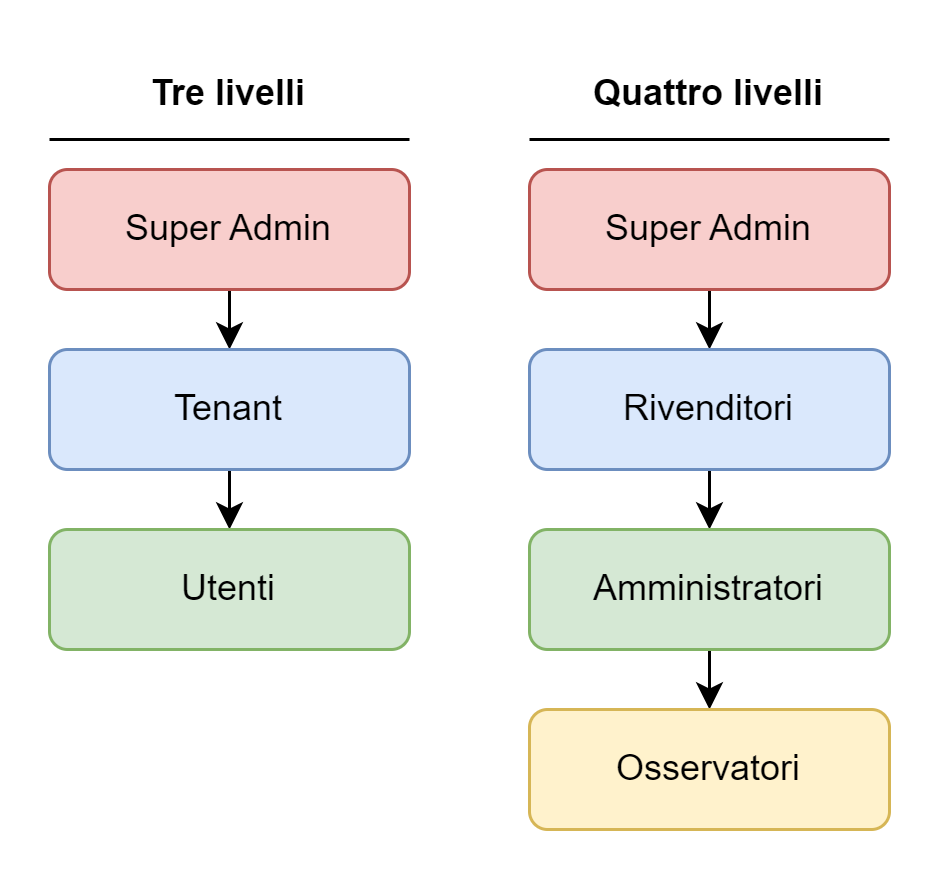
\includegraphics[width=0.6\textwidth]{img/hierarchies.png}
    \caption{Gerarchie di utenti considerate per la funzionalità di multi-tenancy}
\end{figure}

\subsubsection{Gerarchia a quattro livelli}
\label{4-level}
Un'alternativa alla precedente è rappresentata da una gerarchia a quattro livelli, strutturata come segue:

\begin{enumerate}
    \item \textbf{Utenza amministrativa principale}: posizionata al vertice, con poteri illimitati e la facoltà di creare e gestire le utenze sottostanti.
    \item \textbf{Rivenditori / \emph{Reseller}}: queste utenze rappresentano i fornitori del servizio ai clienti finali e possono creare utenti rappresentanti di tali clienti.
    \item \textbf{Clienti amministratori}: utenti che rappresentano singoli clienti privati o amministratori di sistema di aziende. Questi ultimi possono essere responsabili per la sicurezza informatica aziendale o appartenere a dipartimenti specifici, come il CED\footnote{Centro Elaborazione Dati: struttura dedicata alla gestione delle informazioni aziendali in ambito informatico.} o il SOC\footnote{Security Operations Center: centro operativo dedicato alla sicurezza informatica, con focus su risposta agli incidenti e monitoraggio preventivo delle minacce tramite strumenti specifici come SIEM, IDS o IPS.}.
    \item \textbf{Utenti aziendali}: situati all'ultimo livello, questi utenti hanno accesso limitato alle funzionalità del sistema, con la sola possibilità di monitorare e consultare i dati raccolti, senza intervenire sul processo di scansione.
\end{enumerate}

Questa architettura è simile alla precedente, con l'unica aggiunta di un ulteriore livello che consente una visione parziale dei risultati prodotti dal livello immediatamente superiore, senza però poter configurare o modificare alcun parametro del sistema.

\subsection{Limiti d'uso (quote di scansione)}
\label{quote-spec}
Poiché questo progetto è concepito per evolversi in un SaaS (come discusso in \ref{saas}), una parte cruciale del processo di analisi è stata la progettazione di un sistema di controllo delle risorse, eventualmente collegato al modello di pagamento degli utenti.

In prima istanza, è stato considerato un sistema di quote mensili per le scansioni. Una quota, in questo contesto, è definita come un numero intero maggiore di zero ($n > 0$), che indica il numero di nodi scansionabili in un mese dall'utente a cui è attribuita. In termini pratici, la quota corrisponde al numero di indirizzi IP che l'utente può sottoporre a scansione mensilmente utilizzando il servizio.

Le condizioni d'uso specifiche sono le seguenti:
\begin{itemize}
    \item Il numero di scansioni assegnato si rinnova all'inizio di ogni mese, indipendentemente dalla diversa durata dei mesi.
    \item Ogni scansione che coinvolge $n$ indirizzi IP consuma esattamente $n$ unità della quota mensile disponibile.
    \item I nodi non attivi (``spenti'') contano comunque ai fini del decremento della quota.
    \item Scansionare ripetutamente lo stesso indirizzo IP nello stesso mese comporta una riduzione della quota per ogni iterazione della scansione.
    \item Le unità di quota non consumate entro la fine del mese non sono cumulabili per i mesi successivi.
\end{itemize}

Le quote sono stabilite e assegnate dall'utente responsabile per la creazione dell'utenza interessata. Tuttavia, l'effettivo processo di fatturazione al cliente finale non rientra nell'ambito del progetto e si suppone realizzato separatamente.

\subsection{Task di scansione}
Il sistema software dovrebbe consentire la definizione di \emph{task} di scansione su nodi di rete specifici.

L'obiettivo primario di tali task è condurre un \textbf{vulnerability assessment} completo, senza includere elementi di \emph{penetration testing}, sia manuale che semi-automatico.

In aggiunta alla selezione dei bersagli, i task di scansione devono essere configurabili dall'utente per quanto riguarda il livello di dettaglio dei risultati e l'organizzazione temporale delle esecuzioni.

\subsubsection{Temporizzazione e calendarizzazione}
Il sistema deve supportare la definizione di task di scansione ricorrenti, programmabili secondo calendari a cadenza regolare, come quella mensile.

In alternativa, gli utenti devono avere la possibilità di definire task di scansione \emph{ad hoc}, da eseguire una tantum per verifiche specifiche di sicurezza su uno o più nodi.

\subsection{Bersagli}
I bersagli delle scansioni devono poter essere gestiti con la massima flessibilità. Il sistema deve supportare:
\begin{itemize}
    \item Nomi di dominio (DNS);
    \item Indirizzi IPv4 e IPv6;
    \item Insiemi di nodi o indirizzi IP, specificati attraverso notazioni come la CIDR.
\end{itemize}

Inoltre, il sistema deve consentire l'importazione di liste di bersagli tramite file esterni. Questa funzionalità è particolarmente utile in contesti aziendali, dove gli host da analizzare sono spesso numerosi e generati automaticamente da procedure interne, rendendo poco pratico l'inserimento manuale.

\subsection{Risultati}
I risultati delle scansioni devono essere facilmente consultabili, con particolare enfasi su:
\begin{itemize}
    \item La severità delle vulnerabilità rilevate;
    \item Le possibili soluzioni o mitigazioni suggerite;
    \item Altri dettagli tecnici pertinenti, raccolti durante il processo di scansione.
\end{itemize}

Il sistema deve offrire strumenti per filtrare, ordinare e gestire i risultati, garantendo una visualizzazione chiara e intuitiva delle informazioni rilevanti.

\section{Requisiti non funzionali}
Ovvero come il sistema deve comportarsi e a quali standard di qualità, prestazioni, sicurezza e usabilità dovrà conformarsi.

\subsection{Facilità d'uso}
L'interfaccia (UI) e l'esperienza utente (UX) devono essere necessariamente facili e intuitive, con il minor numero possibile di complicazioni esposte all'utente finale.

Il sistema deve pertanto integrare già di per sé dei \emph{default} sicuri e affidabili, lasciando all'utente finale la personalizzazione solo delle parti meno critiche. Il sistema dovrà anche nascondere tutti i dettagli tecnici, ove possibile, limitandosi a mostrare solo lo stretto necessario per comprendere \emph{cosa} e stato trovato e \emph{come} risolverlo (se possibile).

\subsection{Efficienza}
Il sistema deve essere necessariamente efficiente, senza rallentamenti eccessivi nella sua interfaccia. Questo diventa particolarmente critico in sede di reportistica ed analisi dei risultati, dove spesso i dati raccolti da questi sistemi possono accumularsi velocemente.

\section{Requisiti di sistema}
Ovvero quali specifiche tecniche e infrastrutturali dovranno essere rispettate dal sistema in oggetto.

\subsection{Software as a Service}
\label{saas}
Il software che si intende creare sarà a tutti gli effetti un \textbf{SaaS} (Software as a Service). In un modello SaaS, l'applicazione software è installata su uno e più server remoti e vengono fornite agli utenti finali tramite Internet. Il software non viene acquistato, installato e gestito localmente, ma accedono al software e lo usano direttamente, solitamente tramite browser web e a fronte di un abbonamento periodico.

In questo caso specifico la quota di scansione definita in \ref{quote-spec} è il privilegio che viene fornito a fronte del pagamento.

\subsection{Integrazione con scanner esistenti}
Per un componente così complesso e continuamente aggiornato non è realistico pensare di sviluppare da zero un nuovo scanner in grado di competere con le principali soluzioni commerciali. Inoltre, questi sistemi sono ovviamente delicati e critici, giustificando a maggior ragione la scelta di appoggiarsi a soluzioni più mature.

Per queste ragioni, il sistema si integrerà con almeno un altro scanner preesistente. Sarebbe preferibile avere un sistema sufficientemente flessibile da garantire l'interoperabilità con diversi backend di scansione.

Inoltre, lo scanner considerato dovrà necessariamente avere eccellenti doti di interoperabilità con altri sistemi software.

\subsection{Architettura a microservizi}
\label{microservices}
Come spiegato nella precedente sezione, il sistema in oggetto trarrebbe vantaggi dall'essere strutturato in un'architettura non monolitica. Questo sia a carattere di facilità di manutenzione, sia per velocizzare eventuali refactor a seguito di un cambio del backend.

La separazione dei componenti inoltre facilita lo sviluppo di eventuali client, in grado di appoggiarsi alle API esposte dai singoli microservizi.
  \chapter{Greenbone OpenVAS}
  Come backend di scansione si è adottato il framework di \textbf{Greenbone OpenVAS}.

In questo capitolo si vuole spiegare nel dettaglio la struttura e il funzionamento del sistema usato come base del progetto.

\section{Storia del progetto}
\textbf{OpenVAS} (\emph{Open Vulnerability Assessment Scanner}) è una piattaforma \emph{open source} per la rilevazione, l'analisi e la gestione di vulnerabilità e falle di sicurezza.

OpenVAS Nasce nel 2005 come \emph{fork} dello scanner \textbf{Nessus}, quando questi modificò la propria licenza, diventando da \emph{open source} un software proprietario distribuito sotto licenza commerciale. La comunità open source da quel momento ha manutenuto il fork risultante, inizialmente denominato \emph{GNessUs} e poi rinominato in \emph{OpenVAS}. Tempo dopo entrò a far parte dei progetti supportati economicamente dalla \emph{Software in the Public Interest}.

Tra i principali contributori del fork vi erano gli sviluppatori di Intevation e DN-Systems, aziende che poi sarebbero diventate Greenbone AG e finanziate dalla BSI tedesca (l'Ufficio Federale per la Sicurezza Informatica). Eventualmente nel 2008 la neo-costituita Greenbone si propose tra gli obiettivi aziendali il sostenere lo sviluppo open source di OpenVAS e creare delle versioni maggiormente supportate e curate per i clienti enterprise, oltre all'offrire il necessario supporto. Oltre a Greenbone, con il tempo si unirono al progetto altre aziende per contribuire eventualmente ad un feed stabile e aggiornato di test di vulnerabilità, componente chiave ed essenziale dell'intero progetto.

Eventualmente già nel 2010 OpenVAS ruppe la compatibilità con Nessus e negli anni successivi ricevette ulteriore supporto dalla BSI e anche dalla DFN (la rete di ricerca tedesca usata da università e centri di ricerca), nella forma di avvisi di sicurezza regolari pubblicati sotto licenza GPL.

Nel 2017 i contributi di Greenbone diventarono palesi con un cambio di nome ufficiale: il progetto non si sarebbe più chiamato \emph{OpenVAS framework}, ma \textbf{Greenbone Vulnerability Management (GVM)}, un framework completo di sicurezza informatica, dove per OpenVAS si intende solo lo scanner vero e proprio, uno dei tanti componenti.

\section{Modello di business}
Greenbone OpenVAS e GVM possono ricevere gli aggiornamenti di sicurezza e configurazioni da due feed, entrambi manutenuti da Greenbone:
\label{feed}
\begin{itemize}
    \item \textbf{Greenbone Community Feed}: questo canale di aggiornamenti è totalmente gratuito e open-source. Contiene versioni minimali e preconfigurate di configurazioni di scansione, liste di porte, reportistica; ma soprattutto, in questo feed non sono incluse tutti i test di vulnerabilità disponibili, limitandosi a fornire esclusivamente quelli più critici e importanti. I dati sono aggiornati giornalmente secondo una policy di best effort e senza garanzie di alcun tipo.
    \item \textbf{Greenbone Enterprise Feed}: questo canale di aggiornamenti è invece a pagamento, ed è pensato per i clienti di Greenbone che usano il framework GVM in contesti aziendali. In questo canale sono forniti tutti i test di vulnerabilità disponibili, ma anche tutte le configurazioni di scansione e reportistica. Il servizio è inoltre garantito sotto SLA\footnote{\emph{Service Level Agreement}: contratto in cui un provider di un servizio garantisce agli utenti di quel servizio degli standard minimi di qualità e disponibilità.}
\end{itemize}
Il progetto è sostenuto economicamente soprattutto attraverso la sottoscrizione al secondo feed da parte dei clienti di tipo \emph{enterprise}. In aggiunta, Greenbone fornisce anche \emph{hardware appliance}\footnote{Dispositivi fisici progettati per eseguire una specifica funzione / applicazione, ottimizzati espressamente per quell'unico scopo.}, \emph{virtual appliance}\footnote{Sistemi informatici virtuali che eseguono una specifica funzione / applicazione, progettati per essere installati e usati in un software di virtualizzazione.} e una soluzione SaaS gestita direttamente da loro.

\subsection{Greenbone Operating System (GOS)}
Questo sistema operativo è quello che anima le \emph{appliance} fornite da Greenbone. Di fatto è poco più di un insieme di \emph{wrapper} grafici, TUI\footnote{Terminal User Interface} e non, per facilitare la manutenzione del sistema. Il software integra anche il supporto commerciale di Greenbone e vari miglioramenti di esperienza utente.

\section{Architettura}
L'architettura del framework Greenbone Vulnerability Management (GVM) è costituita da numerosi componenti interconnessi.

\subsection{gvmd}
Il demone UNIX \texttt{gvmd} è il cuore del framework GVM. Esso ha compiti di gestione e interconnessione tra tutte le principali componenti di basso livello del sistema, offrendo un'API di gestione operabile con il protocollo \textbf{Greenbone Management Protocol (GMP)}.
\label{gmp}

In particolare:
\begin{itemize}
    \item Comunica con lo scanner OpenVAS vero e proprio tramite il protocollo \textbf{Open Scanner Protocol (OSP)}.
    \item Legge e scrive sul database (di \emph{default} un'istanza di PostgreSQL) i dati ricevuti dai feed configurati, i risultati delle scansioni e il sistema di utenti e ruoli interno al framework GVM.
    \item Fa da server per \textbf{GSA}, l'interfaccia web nativa e ufficiale di Greenbone, di fatto la modalità naturale usata per amministrare l'intero sistema.
\end{itemize}

Si noti che il demone può anche essere operato direttamente senza passare per \textbf{GSA}. Questo è possibile sempre tramite l'API offerta sotto protocollo GMP, consentendo quindi di creare strumenti personalizzati di automazione, ma anche vere e proprie interfacce alternative.

\begin{figure}
    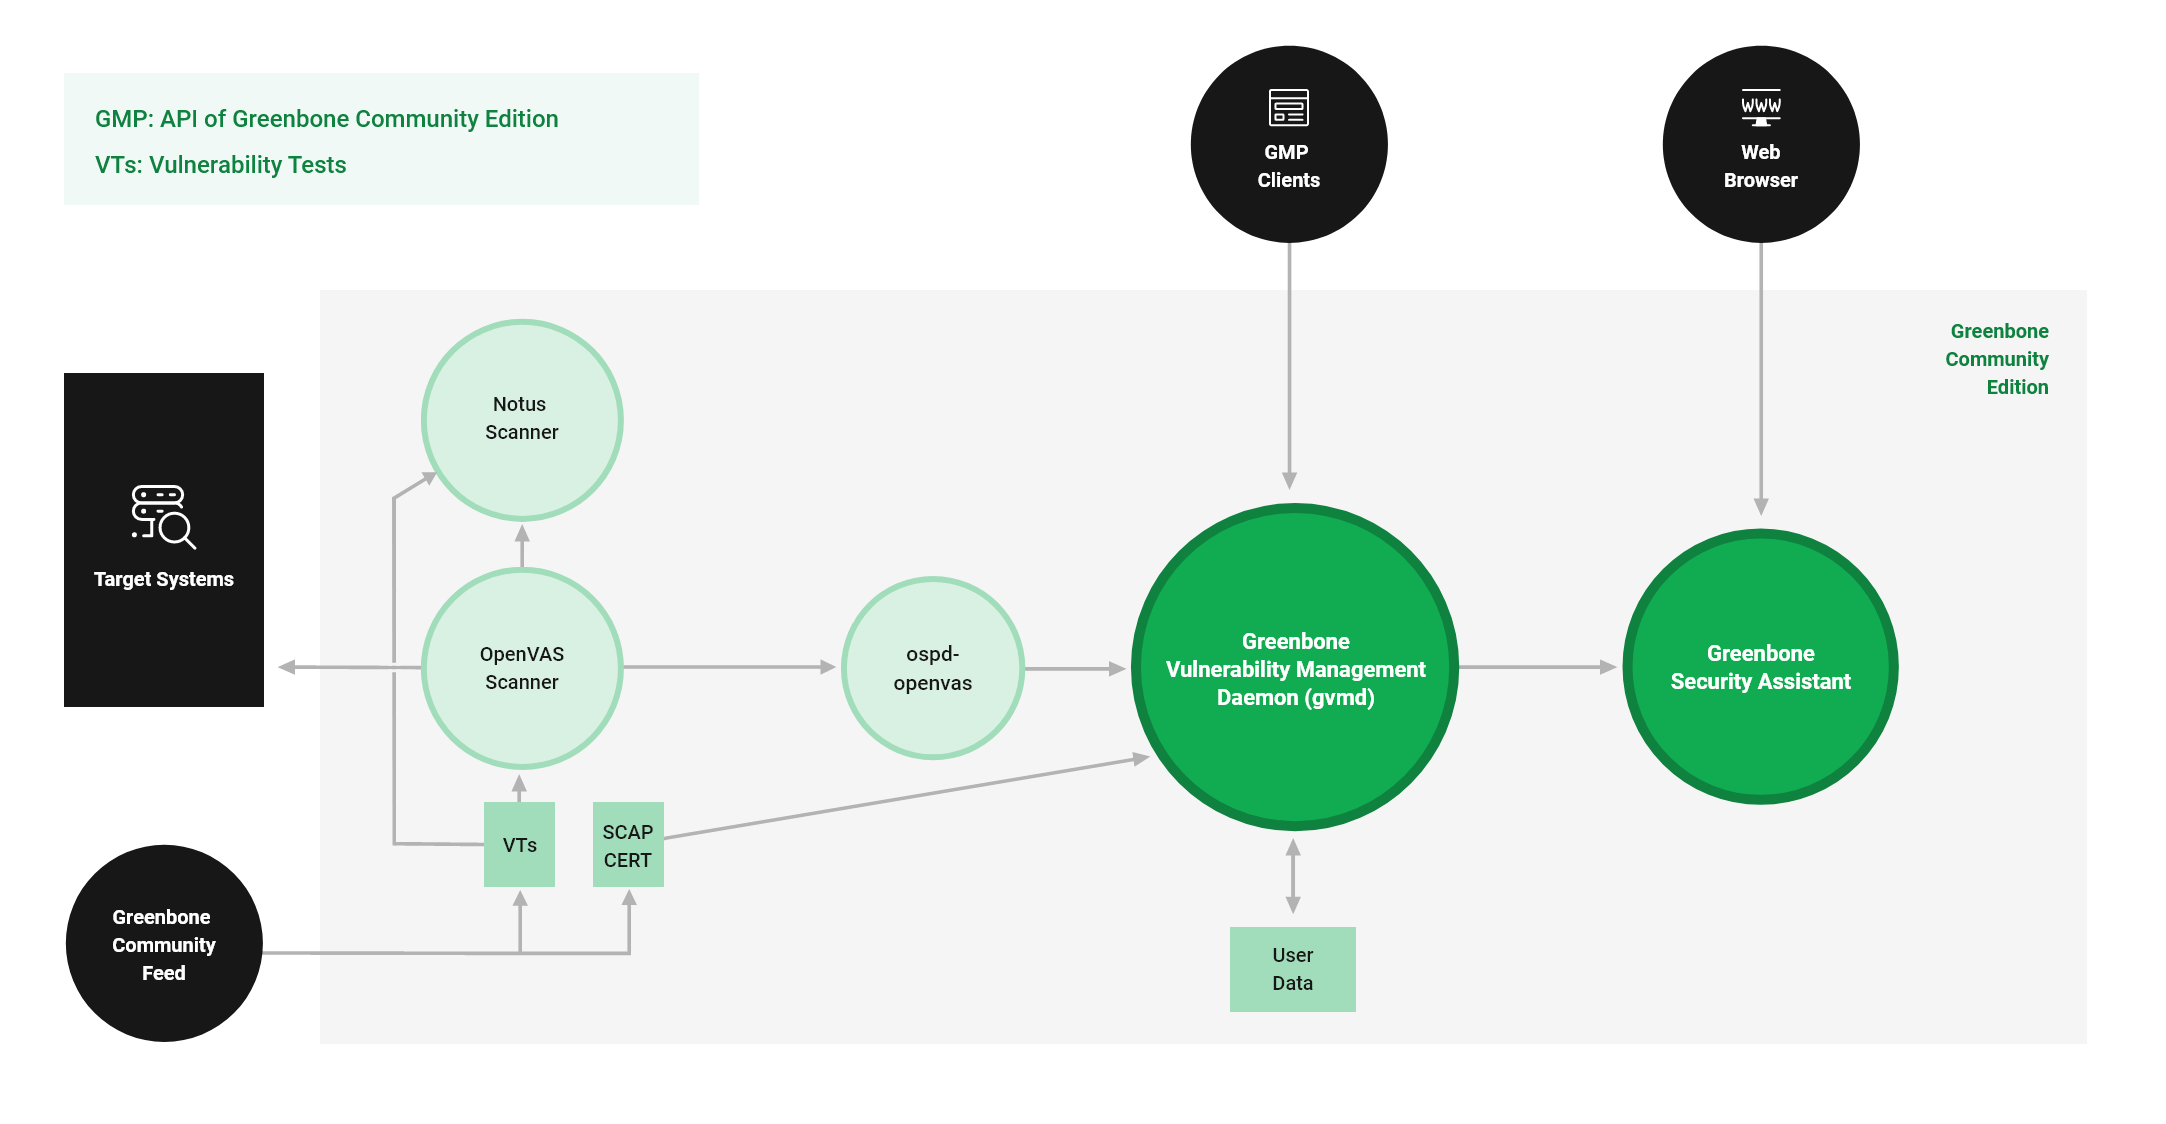
\includegraphics[width=\textwidth]{img/greenbone-community-22.4-architecture.png}
    \caption{Architettura della release 22.4}
\end{figure}

\subsection{GSA}
\textbf{Greenone Security Assistant (GSA)}, ovvero l'interfaccia web nativa di Greenbone (realizzata con React), pensata per l'interazione umana / da parte dell'utente finale attraverso browser.

\subsubsection{gsad}
Si tratta del web server che offre GSA. Di fatto svolge anche le funzioni di backend (che invece fa le veci del semplice frontend). Realizzato interamente in C standard.

\subsection{VT}
Gli scanner veri e propri eseguono delle ``applicazioni'' sui sistemi bersaglio per trovare le vulnerabilità. Questi programmi sono i cosiddetti \textbf{Vulnerability Test (VT)} anche detti talvolta \textbf{Network Vulnerability Test (NVT)}. Essi sono scritti nel linguaggio \textbf{NASL}.

\subsubsection{Linguaggio NASL}
\textbf{NASL (NASL Attack Scripting Language)} è un \emph{Domain Specific Language} interpretato, con lo scopo di definire test per rilevare vulnerabilità su dispositivi di rete. Offre funzioni integrate di supporto per facilitare questo tipo di codifica.

Gli script NASL vengono normalmente eseguiti all'interno delle scansioni OpenVAS, ma possono anche essere eseguiti direttamente dall'utente tramite l'interprete NASL fornito (\texttt{openvas-nasl}).

\subsection{SCAP (CVE, CPE)}
\textbf{SCAP (Security Content Automation Protocol)} è uno standard aperto creato nei primi anni del 2000 dal \textbf{NIST}\footnote{National Institute of Standard and Technology} statunitense, uno dei principali riferimenti attualmente in termini di cybersecurity. Scopo dello standard SCAP è regolare i processi organizzativi di valutazione della sicurezza delle risorse informatiche e quindi automatizzarli.

A tal fine, SCAP comprende un insieme di standard, definiti \textbf{componenti}. Segue una lista dei principali:
\begin{itemize}
    \item \textbf{Common Vulnerabilities and Exposures (CVE)}: fornisce e assegna identificativi univoci alle vulnerabilità note.
    \item \textbf{Common Platform Enumeration (CPE)}: standardizza la descrizione dell'inventario informatico (applicazioni, servizi software, sistemi operativi, hardware) sin nei minimi dettagli.
    \item \textbf{Common Configuration Enumeration (CCE)}: identifica univocamente diverse configurazioni di sistema.
    \item \textbf{Common Vulnerability Scoring System (CVSS)}: valuta la severità di una vulnerabilità attraverso un punteggio $\in [0,10]$.
\end{itemize}

In GVM è integrato un servizio che attraverso i feed menzionati in \ref{feed} aggiorna continuativamente i dati SCAP di cui ha bisogno. In particolare, vengono sfruttati i dati \textbf{CVE} e \textbf{CPE}.

Il framework inoltre mette a disposizione tramite \textbf{GSA} un calcolatore del punteggio \textbf{CVSS}.

\subsection{OpenVAS e Notus}
Lo scanner incluso nel sistema è ovviamente \textbf{OpenVAS}, ma esiste anche un altro ``scanner'' utilizzabile, \textbf{Notus}. Questo in realtà non è nient'altro che un componente Python che razionalizza e ottimizza la verifica degli script NASL.

\subsubsection{openvasd}
Si noti tuttavia che a partire dalla versione 23.0 di OpenVAS è stato introdotto \texttt{openvasd}: questo nell'intenzione di Greenbone vuole essere un unico demone che integra al suo interno tutte le funzioni di OpenVAS (lo scanner vero e proprio), Notus (l'ottimizzazione degli script NASL) e \texttt{ospd-openvas} (l'intermediario che usa il protocollo \textbf{OSP} per mediare la comunicazione tra scanner e \texttt{gvmd}). Il demone sarà riscritto con il linguaggio Rust, per renderlo più performante e moderno, risultando in una migliore manutenibilità. Inoltre, l'API OSP sarà sostituita da una API HTTP.

\section{Altre funzionalità}

\subsection{Scanner CVE / prognosi}
\label{cve}
In aggiunta allo scanner vero e proprio di OpenVAS, Greenbone mette a disposizione un ulteriore scanner ``fittizio'', detto \textbf{CVE}.

Questo scanner di fatto effettua una prognosi della sicurezza del sistema, basandosi sulle informazioni già in suo possesso (ottenute in una scansione precedente; questo di fatto significa che questo scanner può operare solo a seguito di una scansione già conclusa ed efficace di OpenVAS).

In particolare, se OpenVAS è riuscito a popolare i dati di CPE del sistema in oggetto, lo scanner CVE può utilizzare quei dati per stimare la sicurezza al momento attuale della scansione. Questo è fatto semplicemente confrontando i CPE dedotti con i CVE attualmente disponibili.

Si noti che questa scansione è ``fittizia'', poiché di fatto non interagisce mai veramente con il sistema in oggetto (che, ad esempio, nel frattempo potrebbe essere stato aggiornato). Ne segue che i risultati di questo ``scanner'' possano generare falsi positivi con molta più facilità che in una scansione reale e tangibile con OpenVAS. D'altro canto, questa ``scansione'' è quasi istantanea, mentre OpenVAS richiede tempo, risorse computazionali e di rete (che potrebbero scarseggiare in ambienti con un grande numero di host da verificare).

\section{Installazione}
Laddove l'edizione Enterprise è solitamente fornita nelle \emph{appliance}, rendendo di fatto inutile l'installazione, l'edizione gratuita invece deve essere installata dall'utente e configurata secondo le sue esigenze.

Di fatto, esistono due modi in cui il sistema può essere installato e quindi gestito:
\begin{itemize}
    \item \textbf{Compilato da sorgenti}: l'utente deve scaricare il codice sorgente dalle \emph{repository} pubbliche e compilarlo manualmente.
    
    Questo procedimento ovviamente non è consigliato in produzione, visto il rischio di instabilità.
    \item \textbf{Greenbone Community Containers}: in questo formato i singoli componenti precedentemente discussi sono segregati in \emph{container} Docker, garantendo riproducibilità di versioni e funzionalità. Tramite \texttt{docker-compose} i container sono quindi orchestrati e gestiti secondo l'architettura precedentemente esposta.
\end{itemize}

Numerose distribuzioni Linux offrono anche dei pacchetti precompilati nelle loro \emph{repository} native, ma Greenbone ufficialmente non offre supporto per eventuali errori derivanti dall'installazione e dall'uso seguente di queste edizioni, non essendo coinvolta nel processo di compilazione impiegato.

\section{Interoperabilità e protocollo GMP}
Come anticipato in \ref{gmp}, il demone di sistema posto nel cuore del framework Greenbone è in grado di interfacciarsi non solo con i client nativi del sistema (cioè GSA), ma anche con client personalizzati attraverso un protocollo specifico.

Questo protocollo è \textbf{GMP}, un dialetto personalizzato dell'XML e funziona mediante un processo di richiesta - risposta standardizzato con messaggi e attributi specifici.

La comunicazione avviene tramite un punto di accesso comune, rappresentato da una \textbf{socket UNIX}. Lo sviluppatore può interfacciarsi con la socket in oggetto in più modi:
\begin{itemize}
    \item \textbf{Manualmente}, interfacciandosi direttamente con strumenti dedicati e confezionando a mano i messaggi XML secondo lo standard pubblicato da Greenbone.
    \item \texttt{python-gvm}: si tratta di una libreria Python sviluppata e manutenuta direttamente da Greenbone, che realizza una comunicazione semplificata con la socket mascherando il protocollo GMP con un'API Python.
    
    La libreria possiede tutta una serie di vantaggi rispetto all'interfacciamento manuale e a basso livello con la socket:
    \begin{itemize}
        \item Non è necessario creare a mano il messaggio di richiesta XML, ma solo fornire i parametri necessari.
        \item Gestione automatica dell'autenticazione (praticamente tutti i messaggi richiedono un'autenticazione di qualche tipo e anche permessi specifici come vedremo in seguito).
        \item Gli errori sono gestiti in modo integrato con il meccanismo delle eccezioni di Python.
        \item Le risposte sono automaticamente usate per idratare degli oggetti Python della libreria \texttt{lxml}, con integrato il supporto per la manipolazione del documento XML restituito.
    \end{itemize}
    \item \texttt{gvm-tools}: questo strumento esiste soprattutto per gli amministratori di sistema che intendono amministrare OpenVAS da linea di comando e desiderano automatizzare operazioni comuni. In pratica, si appoggia su script realizzati su \texttt{python-gvm}, diventando poco più di un \emph{wrapper} a linea di comando della suddetta libreria.
\end{itemize}

\section{Motivazioni alla base della scelta}
I principali motivi alla base di questa scelta sono:
\begin{itemize}
    \item \textbf{Disponibilità di una versione gratuita}: OpenVAS può essere installato e amministrato direttamente dall'azienda senza costi di licenze o abbonamenti, preoccupandosi solo di predisporre e manutenere l'hardware necessario.
    
    Tuttavia, è importante far notare ancora una volta come la versione gratuita di OpenVAS non disponga di tutti i test di sicurezza disponibili, rendendo necessaria un'ulteriore analisi per verificare se i dati forniti siano sufficienti agli scopi aziendali.

    \item \textbf{Open source}: OpenVAS è open source, perciò il suo codice è liberamente visibile se necessario, evitando durante lo sviluppo il rischio di incorrere in componenti non documentati o comunque opachi.
    
    \item \textbf{Librerie ufficiali}: inoltre, Greenbone mantiene anche degli strumenti ufficiali per interfacciarsi con il sistema OpenVAS, tra cui soprattutto una libreria Python che cerca di implementare quante più funzionalità del protocollo GMP.
\end{itemize}
  \chapter{Progettazione}
  In cui si descrive la progettazione del software a un più basso livello, discutendo le scelte progettuali, le tecnologie e i linguaggi adottati.

\section{Greenbone OpenVAS}
Come backend di scansione per il sistema, inizialmente si è optato per interfacciarsi esclusivamente a \textbf{Greenbone OpenVAS}.

I principali fattori che motivano la scelta di OpenVAS come backend di scansione preferito del progetto includono:

\begin{itemize}
    \item \textbf{Disponibilità di una versione gratuita}: OpenVAS offre una soluzione senza costi di licenza, permettendo all'azienda di occuparsi solo della predisposizione e manutenzione dell'hardware necessario. Tuttavia, è importante notare che la versione gratuita non include tutti i test di sicurezza disponibili, rendendo necessaria una valutazione aggiuntiva per determinare se i dati forniti siano in linea con il \emph{threat model} dell'azienda.

    \item \textbf{Librerie ufficiali}: Greenbone offre strumenti ufficiali che semplificano l'interazione con il sistema OpenVAS e implementano un ampio spettro di funzionalità del protocollo GMP.
    
    \item \textbf{Open source}: OpenVAS è un progetto open source, consentendo la visione e la verifica del codice sorgente. Questo riduce il rischio di essere costretti ad usare componenti non documentati o poco trasparenti.
\end{itemize}

\section{Base di dati}
Il framework di Greenbone già include un suo database interno per la gestione degli utenti e dei ruoli associati ad essi, così come per le scansioni, i risultati e la reportistica. Inoltre, gran parte della logica di business rilevante è già definita e può essere personalizzata con un sistema di permessi abbastanza preciso e granulare, rendendo possibile adattarla facilmente ai nostri scopi.

Per questo motivo, \textbf{si è deciso di non introdurre ridondanza e complessità con un ulteriore database, preferendo invece appoggiarsi sulla base di dati già esistente}.

\subsection{Schema dei dati originale}
Dalla scelta di riutilizzare il database di Greenbone segue che effettivamente sposiamo in tutto e per tutto la struttura dei dati, che è quindi già predisposta per noi.

Lo schema dei dati proposto da Greenbone è strutturato come illustrato in figura \ref{er-crow}\footnote{Si noti che il diagramma ER qui riportato rappresenta solamente le entità d'interesse considerate per il progetto: il reale database contiene uno schema molto più esteso e anche maggiormente interconnesso.}. In particolare:
\begin{itemize}
    \item Una \textbf{Task} rappresenta una scansione predisposta e configurata da un utente (\textbf{User}).
    \item Un utente appartiene ad uno o più ruoli (\textbf{Role}) (nel nostro caso specifico apparterrà sempre a uno ed un solo ruolo). Ogni ruolo inoltre può possedere dei permessi (\textbf{Permission}).
    \item Allo stesso modo, un utente appartiene ad uno o più gruppi (\textbf{Group}) (nel nostro caso specifico l'utente apparterrà al massimo sempre ad un gruppo). Anche i gruppi sono associati a dei permessi.
    \item I permessi sono espressi da un \emph{soggetto} su una \emph{risorsa}. Sia \emph{risorsa} che \emph{soggetto} rappresentano una qualunque entità del sistema, di qualunque tipo.
    \item Ad ogni risorsa possono essere associati uno o più \textbf{Tag} in forma di coppie nome valore. Nel nostro caso useremo questi tag per esprimere la quota dell'utente e pertanto saranno usati solo come decorazione ulteriore dell'entità utente.
    \item Un task è associato a delle preferenze di scansione (\textbf{Preference}). Queste preferenze sono espresse in XML e rappresentano dei dettagli di funzionamento, tra cui soprattutto la \emph{retention policy} dei rapporti generati.
    \item Ogni task è associato a una configurazione di scansione (\textbf{Config}). Questa prescrive in buona sostanza quali VT / NVT vengono eseguiti dalla scansione. Si noti che Greenbone esternamente distingue tra due tipi di configurazione di scansione:
    \begin{itemize}
        \item \emph{Scan config}: ovvero una semplice configurazione definita da un utente umano.
        \item \emph{Policy}: ovvero una scansione prescritta a norma di legge o in ottemperanza a qualche specifico standard. Queste ovviamente andrebbero lasciate così come fornite dal feed.
    \end{itemize}
    Questa distinzione internamente non è gestita con una separazione in entità distinte, come si può vedere dallo schema (allo stesso modo il progetto realizzato non fa distinzioni tra le due tipologie di configurazioni, internamente).

    \begin{figure}[h!]
        \centering
        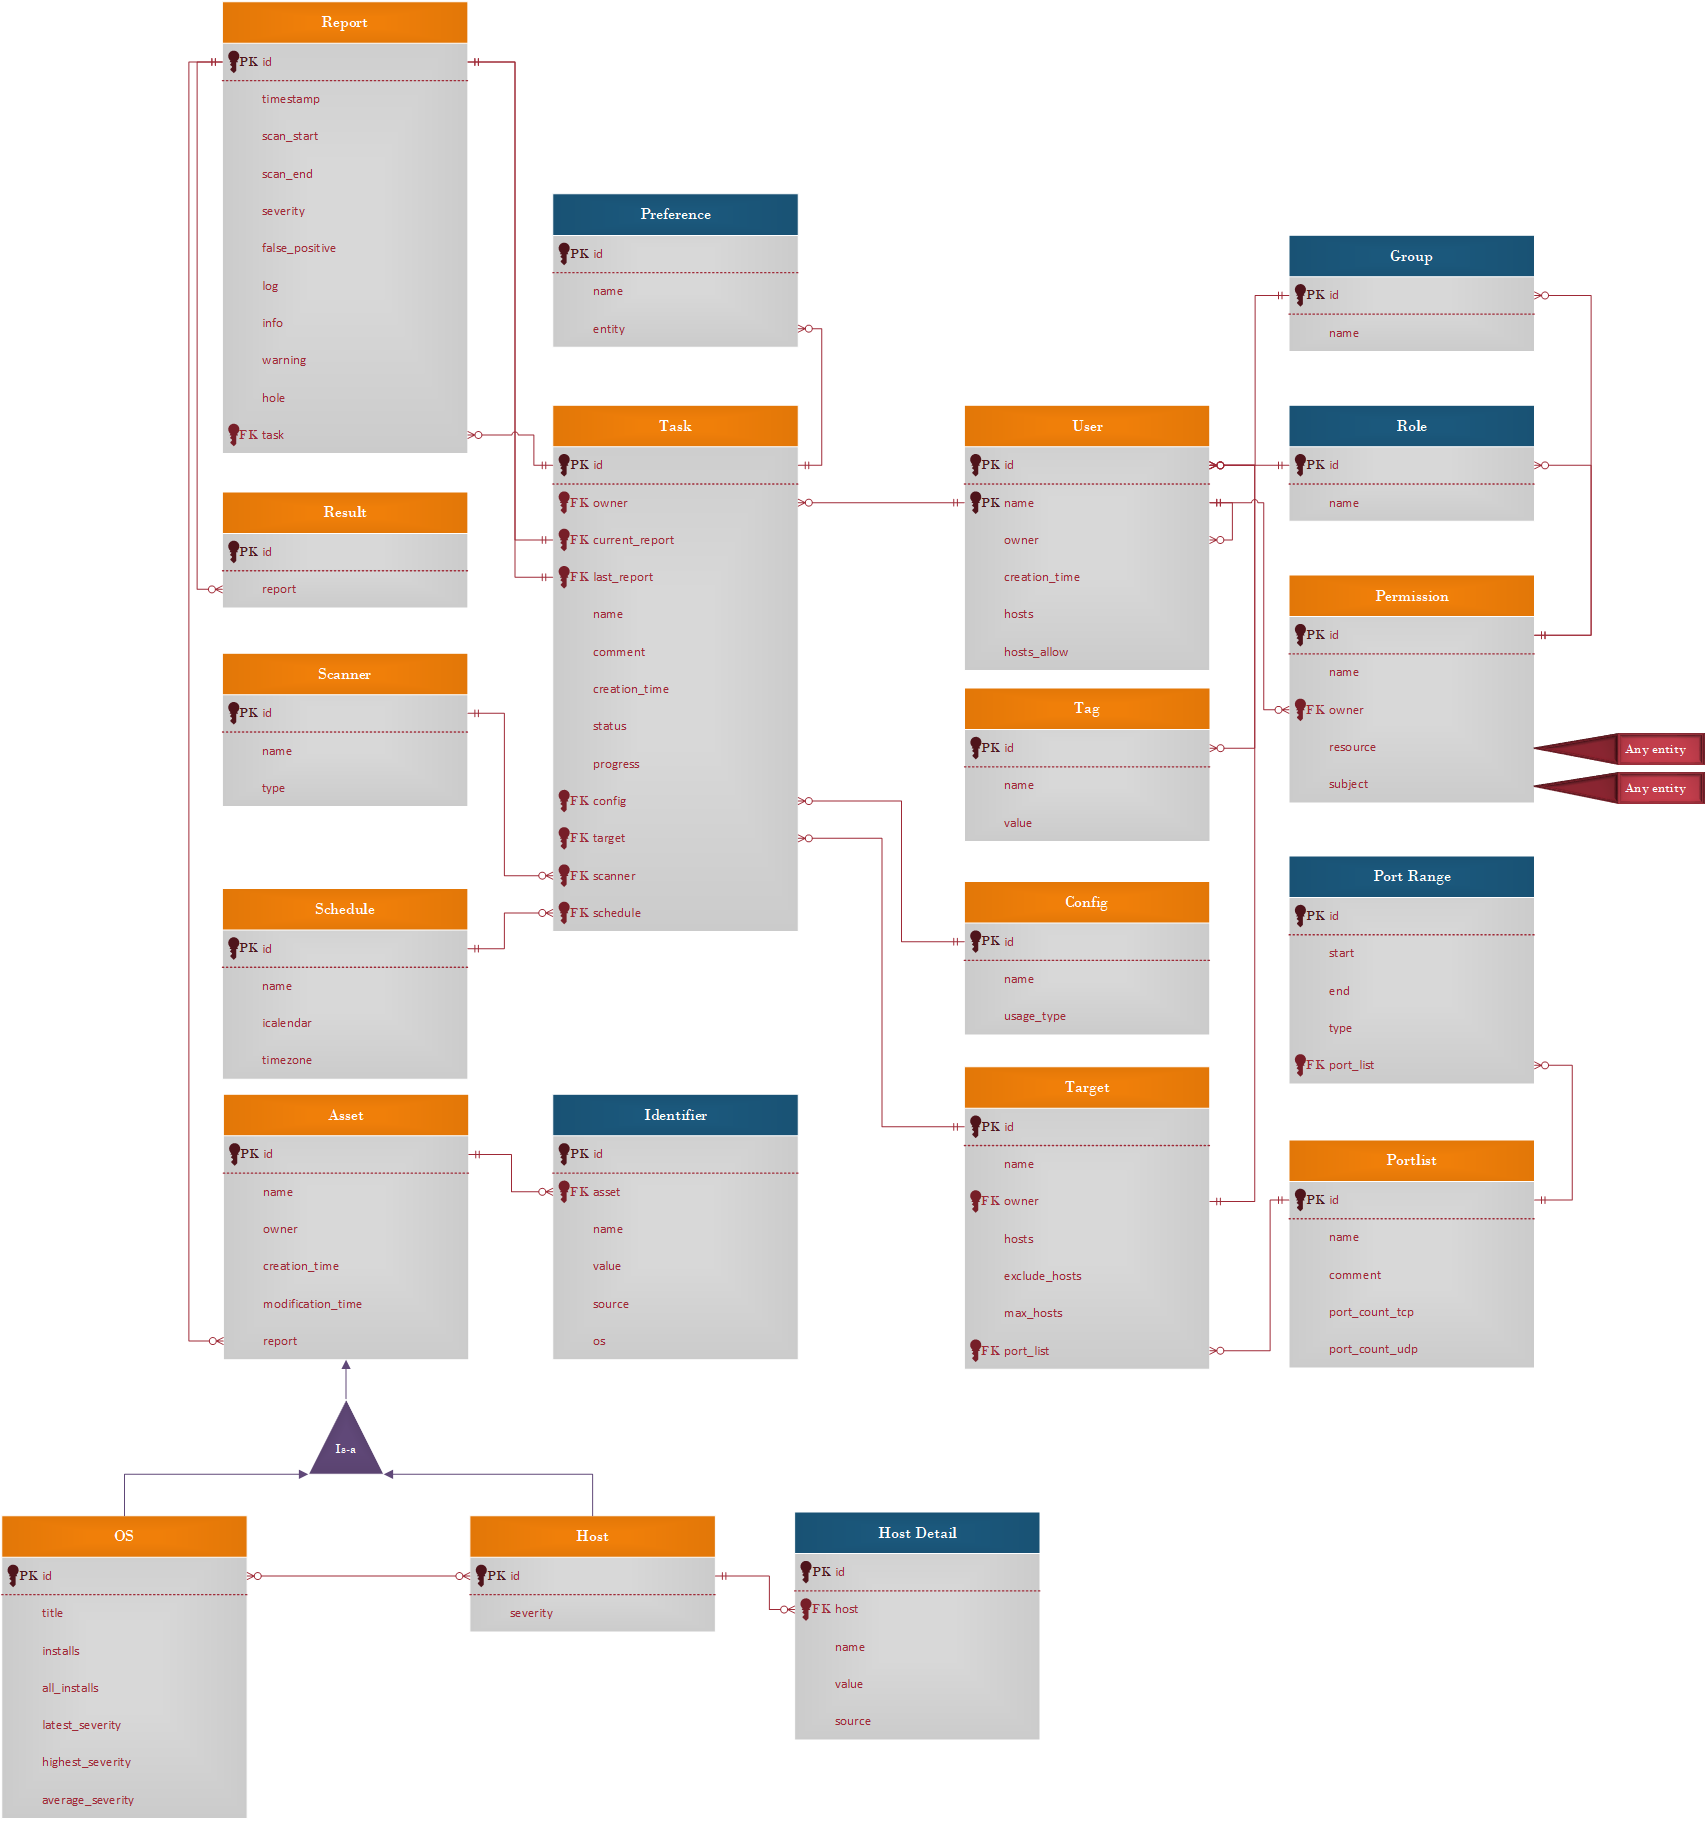
\includegraphics[width=\textwidth]{img/er_crow.png}
        \caption{Schema dei dati d'interesse di GVM}
        \label{er-crow}
    \end{figure}

    \item Ogni scansione viene eseguita su un bersaglio specifico (\textbf{Target}). Un bersaglio di Greenbone OpenVAS specifica uno o più nodi di rete da scansionare, dettagliando anche eventuali credenziali di rete da usare per simulare un attacco di tipo \emph{white box}\footnote{In un attacco / test di tipo \emph{white box} l'attaccante è a disposizione di conoscenza rilevante e approfondita circa l'infrastruttura bersaglio. In un test \emph{black box} invece non viene fornito nessun aiuto / informazione, mentre in un \emph{gray box} vi è una via di mezzo, rappresentando di fatto la tipologia d'attacco più comune.} e le porte da considerare nella scansione.
    \begin{itemize}
        \item Le porte sono definite tramite un'entità \textbf{Portlist} associata. Questa internamente definisce le singole porte in modo efficiente tramite dei \emph{range} divisi per tipo (UDP o TCP).
    \end{itemize}
    \item Un task è eseguito da uno \textbf{Scanner}. In pratica questo è quasi sempre OpenVAS, ma Greenbone mette a disposizione anche uno scanner fittizio detto \textbf{CVE}, già dettagliato in \ref{cve}.
    \item Un task può essere associato anche ad una \textbf{Schedule}, che ne definisce un'eventuale esecuzione futura / ritardata e/o periodica / ricorrente. A basso livello la schedule è espressa tramite standard \textbf{iCalendar} \cite{rfc5545}.
    \item Un task contiene informazioni relative alla sua esecuzione, come il suo stato (in pausa, in esecuzione, in coda, fallita per errore, ecc.) e la percentuale di completamento.
    \item Infine, un task genera uno o più \textbf{Report}. Questi recano informazioni sul periodo temporale a cui sono riferiti e sul numero delle vulnerabilità trovate, nonché la loro severità. Le vulnerabilità si dividono in:
    \begin{itemize}
        \item \textbf{Falsi positivi}: vulnerabilità rilevate dal processo di scansione, ma che lo scanner è riuscito ad identificare autonomamente come falsi positivi.
        \item \textbf{Log}: spesso non sono vere e proprie vulnerabilità, ma semplici informazioni sul sistema di utilità quasi nulla. Alcune di queste sono solitamente disabilitate dagli amministratori di OpenVAS poiché inutilmente paranoiche.
        \item \textbf{Info}: vulnerabilità di basso livello, spesso che forniscono solo informazioni sul sistema, di utilità non nulla.
        \item \textbf{Warning}: vulnerabilità di medio livello, come vecchi standard crittografici ancora in uso, Denial of Service, ecc.
        \item \textbf{Hole / High / Critical}: vulnerabilità o problematiche ad alto livello di rischio e danno potenziale, come RCE, Privilege Escalation, EOL, ecc.
    \end{itemize}
    \item Un rapporto organizza quanto trovato in ``risultati'' (\textbf{Result}). Queste entità contengono metadati che descrivono testualmente la vulnerabilità, l'eventuale soluzione e forniscono gli riferimenti a CVE, CVSS e CPE relativi.
    \item Inoltre, l'esecuzione di un task rivela tutta una serie di \textbf{Asset} che vengono scoperti e inventariati durante la realizzazione del rapporto. Questi sono principalmente:
    \begin{itemize}
        \item \textbf{Host}, ovvero macchine fisiche o virtuali (questo comportamento può essere personalizzato come opzione dello scanner).
        \item Sistemi operativi (\textbf{OS}), con vari gradi di precisione nel loro processo di \emph{fingerprinting}.
    \end{itemize}
\end{itemize}

\section{Architettura}
Come anticipato in \ref{microservices}, in fase di analisi è emersa la necessità di realizzare sin dall'inizio un sistema modulare e disaccoppiato. Da un punto di vista puramente teorico e di architettura si deducono i seguenti sistemi con le seguenti funzionalità:
\begin{itemize}
    \item Uno o più backend di scansione. Come già detto, si vuole usare \textbf{OpenVAS} per questo componente, riservando l'integrazione con altri backend a sviluppi futuri.
    \item Un sistema che fa da interconnessione e adattatore tra il backend di scansione, introducendo un livello di indirezione e fornendo funzionalità ad un sistema \emph{user-facing} attraverso un'API unificata.
    \item Il sistema di interfaccia, che si interconnette con l'adattatore di cui sopra per fornire un \emph{frontend} facilitato e moderno per l'uso da parte dell'utente finale.
\end{itemize}

\begin{figure}
    \centering
    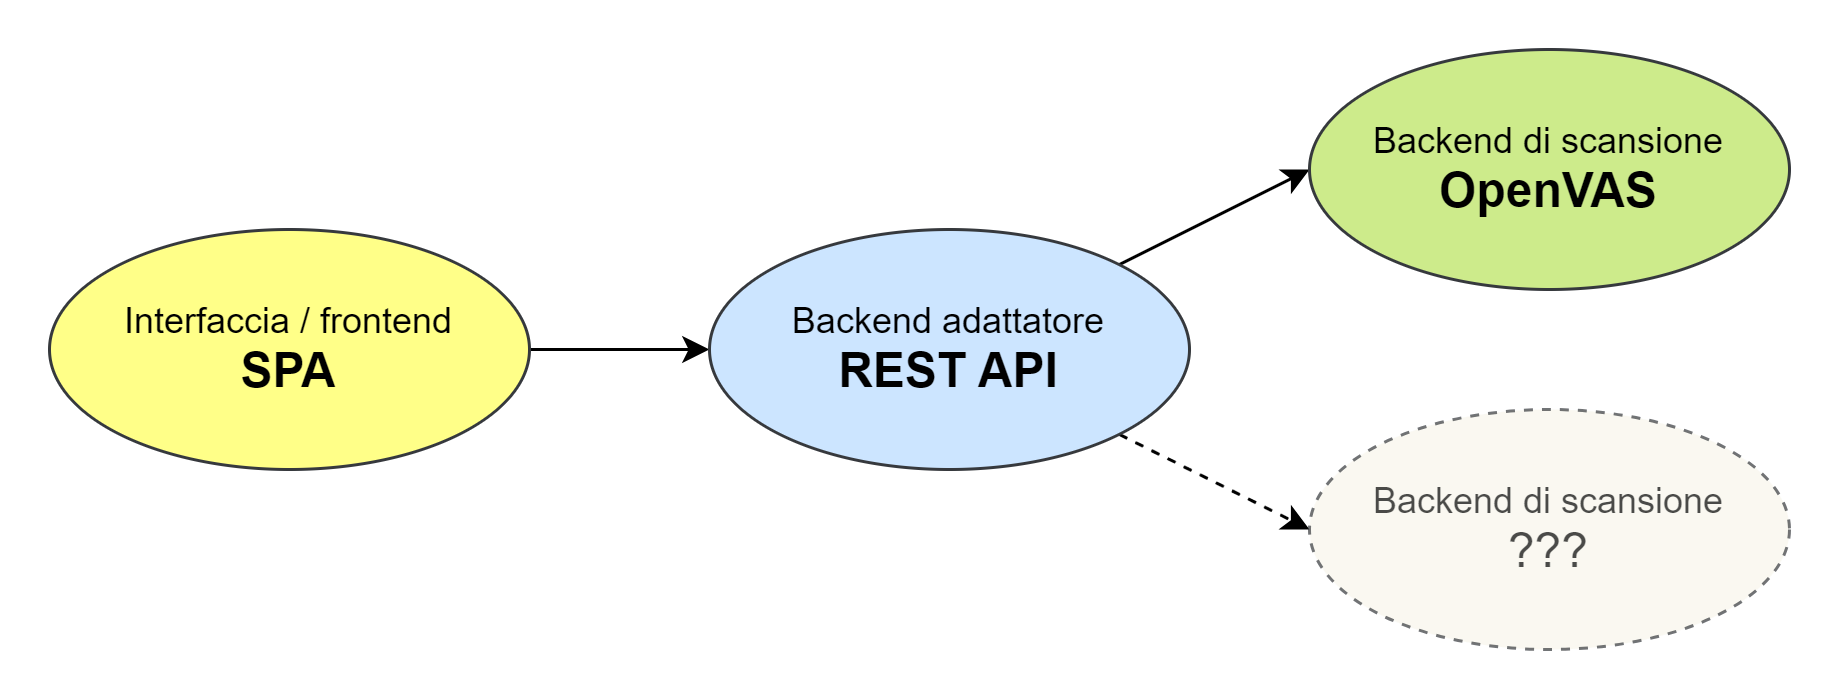
\includegraphics[width=0.8\textwidth]{img/systems-highlevel.png}
    \caption[Architettura globale / ad alto livello dei componenti del sistema]{Architettura globale / ad alto livello dei componenti del sistema. Il backend adattatore lascia aperta la possibilità di integrazione con sistemi differenti da OpenVAS mantenendo un'unica interfaccia}
\end{figure}

Tenuto conto delle moderne tendenze di sviluppo, dei framework supportati e della necessità di avere un sistema \emph{cross-platform}, si è deciso per sviluppare gli ultimi due sistemi tramite un'\textbf{applicazione web} composta da due parti distinte ricalcanti rispettivamente gli scopi dei sistemi sopracitati:
\begin{itemize}
    \item Un \emph{backend} realizzato in forma di \textbf{REST API}. Questo si appoggerà sul database interno di Greenbone OpenVAS indirettamente attraverso il protocollo GMP.
    \item Un \emph{frontend} realizzato in forma di \textbf{SPA}, che sfrutta il backend per interagire con il sistema di scansione.
\end{itemize}

\section{REST API di Backend}
REST è un paradigma ormai molto popolare di sviluppo delle API web. Una REST API spesso non implementa tutto lo standard REST, ma quanto segue sono solo le specifiche più comuni e popolarmente identificate come minime:
\begin{itemize}
    \item \textbf{Stateless}: ogni richiesta del client deve contenere tutte e sole le informazioni necessarie a comprendere la richiesta. In teoria il server non dovrebbe avere bisogno di mantenere uno stato per rispondere alla maggior parte delle richieste. L'autenticazione è gestita pertanto mediante token di accesso, ma in pratica questo aspetto dello standard è modificato per usare i cookie di sessione, specie quando la REST API è consumata esclusivamente da client web come una Single Page Application (scenario sempre più comune, per quanto degenere rispetto agli scopi originali dello standard).
    \item Le entità del sistema sono rappresentate come \textbf{risorse}, identificate dallo URL e da formati specifici come JSON (usato per questo progetto) o XML.
    \item La semantica delle operazioni eseguibili sulle risorse è sottintesa dai \textbf{metodi HTTP} utilizzati (GET per ottenere la/e risorsa/e, POST per crearne di nuova, PUT / PATCH per aggiornare le risorse, DELETE per rimuoverne).
\end{itemize}

\subsection{Linguaggio di programmazione}
Dall'analisi delle librerie offerte da Greenbone per l'interconnessione dei suoi sistemi, effettuata in \ref{libraries}, emerge chiaramente la superiorità in quest'ambito del linguaggio \textbf{Python}, semplicemente per la presenza di una libreria software ufficialmente manutenuta e supportata.

Infatti, utilizzare un linguaggio di programmazione diverso dal Python imporrebbe la necessità di sviluppare e manutenere in proprio una libreria che faccia da \emph{client} per la socket UNIX, dialogando con il protocollo GMP, realizzando di fatto un doppione di una libreria già esistente, solo per un altro linguaggio.

Inoltre, sarebbe necessario implementare da zero lo schema dei dati descritto dal protocollo, aggiungere funzionalità di \emph{parsing}, controllo degli errori, ma soprattutto andrebbe aggiornando di volta in volta di pari passo con gli aggiornamenti al protocollo GMP.

Per tutti questi motivi, si è considerato l'uso di \texttt{python-gvm} come una scelta quasi obbligata. L'unico vantaggio che poteva portare l'uso di una libreria sviluppata indipendentemente era l'integrazione diretta di una traduzione dal linguaggio XML in una struttura dati più ricca, di fatto realizzando un \textbf{ORM} a livello di libreria di interconnessione con la base dati (qua indirettamente rappresentata dal protocollo GMP). Questa funzione di traduzione non è implementata dalla libreria \texttt{python-gvm}, rendendo di fatto obbligatoria una piccola parte di gestione aggiuntiva a livello di modello\footnote{``Modello'' inteso nel senso del \emph{design pattern} \textbf{MVC, Model View Controller}, secondo il quale un'applicazione può essere scomposta in una parte di accesso e gestione dei dati (\emph{model}) e una parte di interfaccia (\emph{view}), mediate unicamente da un livello di interconnessione il più possibile semplice e minimale (\emph{controller}).} dei dati.

\subsection{Framework}
Per un progetto destinato ad un uso professionale è imperativo utilizzare un \emph{framework}, per garantire soprattutto sicurezza, facilità di manutenibilità e anche di sviluppo.

Avendo scelto il linguaggio Python, emergono soprattutto tre framework sufficientemente manutenuti e utilizzati da poter essere comparati:
\begin{itemize}
    \item \textbf{Django} è un framework web ad alto livello che incoraggia lo sviluppo rapido e un design pulito e pragmatico. Di fatto è il framework web full-stack più popolare in ambito Python, comparabile con Laravel e Ruby on Rails per gli ecosistemi rispettivamente PHP e Ruby.
    
    Django offre una serie di funzionalità integrate per accelerare lo sviluppo, come un proprio ORM (Object-Relational Mapping), un sistema di autenticazione, un pannello di amministrazione automatico e strumenti per la gestione delle migrazioni del database. Utilizza un'architettura Model-Template-View, che separa la logica di business dalla presentazione in modo simile all'architettura MVC, e include protezioni contro attacchi comuni come SQL injection, cross-site scripting (XSS) e cross-site request forgery (CSRF).
    \item \textbf{Flask} è un micro-framework leggero e flessibile per Python, progettato per essere semplice e facile da estendere. Esso fornisce solo le funzionalità di base, lasciando agli sviluppatori la libertà di scegliere individualmente le singole librerie e gli strumenti da utilizzare. La sua architettura minimalista lo rende ideale per progetti più piccoli o per applicazioni che richiedono una personalizzazione significativa. Grazie alla sua semplicità, è spesso utilizzato per sviluppare prototipi, applicazioni minimali o dal design particolarmente esotico, e può essere facilmente esteso con numerosi plugin e librerie di terze parti.
    \item \textbf{FastAPI} è un framework moderno e veloce per costruire API con Python 3.6+ fortemente basato sullo standard \textbf{OpenAPI}. È progettato per essere altamente performante e facile da usare. FastAPI poggia sul framework web Starlette e la libreria Pydantic, che tramite le annotazioni di Python fornisce di default una validazione automatica dei dati. Inoltre, FastAPI supporta la generazione automatica e auto-aggiornante di una documentazione interattiva delle API sviluppata, grazie allo standard OpenAPI e Swagger UI o ReDoc. Infine, supporta anche la programmazione asincrona, a differenza di tutti gli altri framework.
\end{itemize}
In questo progetto si è deciso per l'adozione del framework \textbf{Flask} \cite{flask}, sulla base di una serie di considerazioni tecniche e pratiche che ne evidenziano l'idoneità rispetto alle altre opzioni disponibili:

Infatti, sebbene Django offra un ecosistema robusto e completo, è principalmente orientato verso applicazioni full-stack monolitiche e non si presta in modo ottimale alla creazione di REST API, nonostante l'esistenza di Django Rest Framework. Quest'ultimo, infatti, suggerisce che il framework non è stato concepito in partenza con questo scopo primario in mente.

D'altra parte, FastAPI è un framework moderno progettato specificamente per la creazione di REST API, presentandosi sullo spettro opposto rispetto a Django, ma presenta altre limitazioni significative. La mancanza di un'API pubblica per i suoi componenti rende il progetto meno affidabile nel lungo termine, specialmente per applicazioni di grande rilevanza. Inoltre, la gestione della codebase lasciata in gran parte nelle mani di un singolo sviluppatore solleva interrogativi sulla sostenibilità del progetto.

Flask, al contrario, si distingue per la sua flessibilità rendendolo particolarmente adatto per il caso specifico, che non prevedendo un database risulta abbastanza peculiare. Tra l'altro, sotto questo aspetto si discosta nettamente da FastAPI e Django, che possono risultare eccessivamente rigidi e guidati.

Flask consente di plasmare l'applicazione secondo le specifiche esigenze del progetto, grazie ad un ecosistema di estensioni molto florido. Segue ora in che modo queste estensioni sono state scelte a livello architetturale.

\subsection{Validazione dei dati e API REST}
Questo consente tra l'altro di replicare le funzionalità più avanzate di FastAPI, come la validazione dei dati e la generazione automatica della documentazione.

Queste funzionalità sono replicate in Flask attraverso l'uso di plugin ben mantenuti dalla comunità:
\begin{itemize}
    \item La validazione dei dati è gestita con la libreria \textbf{Marshmallow} \cite{marshmallow}, integrata in Flask con un'estensione che funge da collante tra le librerie.
    \label{design-marshmallow}
    \item \textbf{APIFlask} \cite{apiflask} invece è un plugin / framework secondario che funge da wrapper rispetto a Flask. Il suo scopo è facilitare la creazione di API, ma integrano anche la generazione automatica di specifiche OpenAPI \cite{openapi-specification} e documentazione interattiva tramite Swagger UI, ReDoc e non solo.
\end{itemize}

\subsection{Autenticazione e sicurezza}
La sicurezza del backend di una REST API è un aspetto fondamentale da considerare durante lo sviluppo di un'applicazione web e questa non fa eccezione. Esistono diversi metodi per autenticare una REST API, tra cui l'uso di \textbf{token di accesso} e \textbf{cookie di sessione}. Ogni approccio presenta vantaggi e svantaggi in termini di facilità d'uso e sicurezza, e la scelta del metodo più appropriato dipende dalle specifiche esigenze del progetto.

Nel contesto di questo progetto, è stata presa la decisione di utilizzare i cookie di sessione per l'autenticazione. Questo metodo si distingue per la sua semplicità e sicurezza:
\begin{itemize}
    \item A differenza dei token di accesso, che devono essere inclusi manualmente in ogni richiesta HTTP, \textbf{i cookie di sessione vengono gestiti automaticamente dal browser}. Ciò significa che il programmatore non deve preoccuparsi di inviare il token ad ogni richiesta, semplificando notevolmente lo sviluppo dell'applicazione.
    \item Inoltre, i cookie di sessione possono essere configurati con attributi di sicurezza come \texttt{Secure}, \texttt{HttpOnly} e \texttt{SameSite}:
    \begin{itemize}
        \item L'attributo \texttt{Secure} garantisce che il cookie venga trasmesso solo su connessioni HTTPS. Questo significa che le informazioni contenute nel cookie non possono essere intercettate durante il transito tra il client e il server, proteggendo così i dati sensibili da attacchi di tipo man-in-the-middle. Senza questo attributo, i cookie potrebbero essere inviati anche su connessioni non sicure, esponendo le informazioni a potenziali attaccanti.
        \item L'attributo \texttt{HttpOnly} impedisce l'accesso al cookie tramite JavaScript. Questo è particolarmente importante per proteggere i cookie da attacchi di cross-site scripting (XSS), in cui un attaccante potrebbe tentare di eseguire codice malevolo nel contesto del browser dell'utente. Se un cookie è contrassegnato come HttpOnly, anche se un attaccante riesce a iniettare codice JavaScript nella pagina, non sarà in grado di accedere al contenuto del cookie, riducendo significativamente il rischio di furto di sessione.
        
        Se invece si usano i token è necessario maneggiarli con JavaScript per introdurli nelle richieste, di fatto introducendo un'ulteriore superficie d'attacco (XSS, appunto). Una mitigazione sarebbe istruire il server per fornire il token in un cookie \texttt{HttpOnly}, ma non tutte le librerie di gestione dei token supportano trasparentemente questa pratica, rendendo necessaria l'implementazione di codice ``collante'' che introduce ulteriori rischi di security. Sotto questo punto di vista la natura personalizzabile e spoglia di Flask ha favorito la nascita di un'ecosistema frammentato e senza ancora una libreria di sicurezza standard.
        \item Infine, l'attributo \texttt{SameSite} offre una protezione contro attacchi di cross-site request forgery (CSRF). Questo attributo consente di specificare se il cookie deve essere inviato con richieste provenienti da siti esterni. Impostando SameSite su \texttt{Strict} o \texttt{Lax}, il cookie non verrà inviato con richieste che non provengono dallo stesso dominio, limitando così le possibilità di attacchi CSRF.
        
        Nel progetto in oggetto si è comunque implementato un token CSRF per ulteriore scrupolo, grazie al framework \texttt{WTForms} sviluppato dai manutentori di Flask.
    \end{itemize}
    \item La possibilità di effettuare il logout in modo semplice e diretto rappresenta un ulteriore vantaggio di questo approccio, senza la necessità di dover introdurre \emph{blacklist} o simili stratagemmi, pratica invece comune quando si lavora con token web.
\end{itemize}

Sebbene l'uso di token di accesso offra vantaggi significativi, come una maggiore scalabilità in contesti distribuiti e la necessità di supportare client diversi da un browser, queste problematiche sono considerate distanti nel progetto qui considerato e potrebbero per giunta non rivelarsi mai rilevanti. L'autenticazione web, invece, è un aspetto certo e inevitabile, e la scelta di cookie di sessione si allinea perfettamente con le esigenze attuali del progetto.

Tuttavia, è importante notare che nulla vieta di adottare un approccio ibrido, simile a quello per esempio della popolare libreria ufficiale Sanctum del framework Laravel, che supporta entrambi i sistemi di autenticazione, cookie e token. In questo modo, si utilizzano i cookie di sessione per le applicazioni web a pagina singola (SPA), come nel nostro caso, e i token di accesso rimarrebbero a disposizione degli altri client, come le applicazioni mobili. Questa strategia consentirebbe di sfruttare i vantaggi di entrambi i metodi, garantendo una maggiore flessibilità e adattabilità alle diverse esigenze degli utenti e dei dispositivi.

La libreria scelta per gestire questo ambito è la popolare e open-source \texttt{flask-login} \cite{flask-login}.

\subsection{Gestione sessioni}
La gestione delle sessioni è un aspetto cruciale nello sviluppo di applicazioni web, e la scelta del metodo di memorizzazione delle sessioni può influenzare significativamente la sicurezza e le prestazioni dell'applicazione. Di default, Flask utilizza esclusivamente sessioni \emph{client-side}, il che significa che i dati della sessione vengono memorizzati direttamente nei cookie del browser dell'utente. Questo approccio comporta che ogni volta che il client effettua una richiesta al server, il cookie contenente le informazioni della sessione viene inviato insieme alla richiesta. Sebbene questo metodo possa sembrare semplice e immediato, presenta alcune limitazioni, tra cui il fatto che i dati di sessione sono visibili a chiunque, siccome la crittografia usata per il cookie non garantisce la confidenzialità dei dati al suo interno, ma solo la sua integrità.

Per superare queste limitazioni, si è deciso per l'uso di \texttt{flask-session}, una libreria che consente a Flask di gestire sessioni \emph{server-side}. Con le sessioni server-side, i dati della sessione vengono memorizzati sul server, mentre il client riceve nel cookie solamente un identificatore univoco della sessione. Questo approccio offre numerosi vantaggi in termini di sicurezza, poiché i dati sensibili non vengono mai esposti al client. Inoltre, consente una gestione più efficiente delle sessioni, poiché il server può mantenere lo stato dell'utente senza dover inviare continuamente informazioni sensibili attraverso la rete.
Rimane comunque necessario difendersi da attacchi come la \textbf{Session Fixation} \cite{flask-session}.

Per implementare le sessioni \emph{server-side} di Flask Session, si è deciso per l'uso di \textbf{Redis} \cite{redis}, un sistema di archiviazione in memoria, strutturato come un database chiave-valore, noto per la sua velocità e leggerezza. È particolarmente adatto per la gestione delle sessioni o di piccole \emph{cache}, poiché consente un accesso rapido e scalabile ai dati memorizzati. Inoltre, Redis è ampiamente supportato dalla libreria scelta ed è attivamente sviluppato, il che scongiura rischi di integrazione.

\subsection{CORS e DotEnv}
Durante lo sviluppo locale dell'applicazione, è emersa la necessità di gestire le richieste in regime di \textbf{Cross-Origin Resource Sharing (CORS)}. CORS è un meccanismo di sicurezza implementato nei browser che consente o limita le richieste effettuate da un'origine (domain) a un'altra. Questo è particolarmente rilevante quando si sviluppano applicazioni web che interagiscono con API o risorse ospitate su domini diversi, e negli ambienti di sviluppo è comune. Senza una corretta configurazione di CORS, il browser bloccherebbe automaticamente le richieste provenienti da origini non autorizzate, impedendo così il corretto funzionamento dell'applicazione. Per affrontare questa problematica, è stata utilizzata un'estensione di Flask specificamente progettata per gestire CORS (\texttt{Flask-CORS}), che consente di configurare facilmente le politiche di accesso e di specificare quali origini sono autorizzate a interagire con l'API.

In aggiunta alla gestione di CORS, è fondamentale considerare che molte funzionalità dell'applicazione possono variare a seconda dell'ambiente in cui si trova (come CORS stesso; come si vedrà nell'installazione finale dettagliata in \ref{cors-deployment} non sarà necessario usarlo). Ad esempio, alcune funzionalità potrebbero essere attivate in fase di sviluppo, ma disattivate in produzione per motivi di sicurezza o prestazioni. Per gestire in modo efficace queste configurazioni environment-dependent, è stato adottato lo standard \textbf{DotEnv}, ovvero uno dei modi più popolari per realizzare i principi di una cosiddetta applicazione a 12 fattori \cite{12-factor}. DotEnv è una convenzione per la gestione delle variabili di ambiente, che consente di definire configurazioni specifiche per ciascun ambiente in file di testo semplici, solitamente denominati \texttt{.env}. Questi file contengono coppie chiave-valore che possono essere facilmente lette dall'applicazione al momento dell'avvio.

L'integrazione di DotEnv con Flask è facilitata da un'altra estensione, \texttt{Flask-DotEnv}, che consente di caricare automaticamente le variabili di ambiente definite nel file .env all'interno dell'applicazione. Questo approccio non solo semplifica la gestione delle configurazioni, ma migliora anche la sicurezza, poiché consente di mantenere informazioni sensibili, come chiavi API e credenziali di accesso, al di fuori del codice sorgente (i file .env non sono mai aggiunti al sistema di controllo della versione, ma solo una loro versione di esempio, nel caso specifico denominata \texttt{.env.example}). In questo modo, è possibile evitare di esporre dati sensibili in repository pubblici o in ambienti di sviluppo condivisi.

\section{SPA di Frontend}
Una \textbf{SPA (Single Page Application)} è un tipo di applicazione web che carica una singola pagina HTML e aggiorna dinamicamente il contenuto in risposta alle interazioni dell'utente, senza la necessità di ricaricare l'intera pagina. Questo approccio migliora notevolmente l'esperienza utente, poiché consente transizioni più fluide e tempi di risposta più rapidi, rendendo l'applicazione più reattiva e simile a un'applicazione desktop, cosa desiderata per il progetto in questione.

\subsection{Scelta tra SPA e rendering ibrido}
In alternativa alla scelta di sviluppare una SPA, si sarebbe potuto considerare un approccio di rendering ibrido, come quello offerto da Inertia.js o librerie simili. Questo tipo di soluzione consente di combinare le caratteristiche delle applicazioni tradizionali con quelle delle SPA, permettendo di costruire interfacce utente moderne senza dover gestire un'API REST separata. Tuttavia, è importante notare che, attualmente, non esistono librerie ben supportate per Flask che offrano un'integrazione simile a quella di Inertia.js con Laravel, limitando così le opzioni disponibili per implementare questo approccio.

Un ulteriore aspetto da considerare è che l'adozione di un rendering ibrido tenderebbe a riconnettere le componenti dell'applicazione, accoppiando di fatto la SPA e la REST API in un'unica architettura monolitica. Questo contrasta con l'obiettivo iniziale del progetto, che era quello di disaccoppiare il frontend dal backend, consentendo una maggiore flessibilità e scalabilità. La separazione delle preoccupazioni tra client e server è fondamentale per garantire che ciascuna parte dell'applicazione possa evolversi indipendentemente, facilitando aggiornamenti e manutenzione senza influenzare l'altra componente.

\subsection{Framework}
Nella selezione del framework, si sono confrontati i tre framework più popolari e ampiamente manutenuti: \textbf{Angular}, \textbf{React} e \textbf{Vue.js}.

Tutti questi framework servono allo scopo di costruire interfacce utente nel modo più semplice e standardizzato possibile, tipicamente mediante le seguenti comuni caratteristiche:
\begin{itemize}
    \item \textbf{Pattern MVVM (Model-View-ViewModel)}: Questi framework seguono il pattern MVVM, che separa la logica di business (Model) dalla presentazione (View) e gestisce l'interazione tra i due attraverso un ViewModel. Questo approccio consente una chiara separazione dei compiti, facilitando la manutenzione e l'estensibilità del codice.
    
    \item \textbf{Reattività}: I framework implementano un sistema reattivo che consente di aggiornare automaticamente la vista quando i dati cambiano. Questo significa che gli sviluppatori possono definire legami tra i dati e la UI, riducendo la necessità di manipolazioni manuali del DOM e migliorando l'efficienza dell'applicazione. Anzi, in questi framework manipolare direttamente il DOM è spesso visto come un \emph{anti-pattern}.
    
    \item \textbf{Separazione in Componenti}: Angular, React e Vue promuovono un'architettura basata su componenti, in cui l'interfaccia utente è suddivisa in parti riutilizzabili e modulari. Ogni componente gestisce il proprio stato e la propria logica, facilitando la riusabilità e anche la verificabilità della correttezza del codice.
    
    \item \textbf{Virtual DOM}: React e Vue utilizzano un Virtual DOM, una rappresentazione in memoria del DOM reale, per ottimizzare le operazioni di aggiornamento. Questo approccio consente di ridurre il numero di manipolazioni dirette del DOM, migliorando le prestazioni complessive dell'applicazione.
    
    \item \textbf{Routing}: La maggior parte di questi framework offre soluzioni integrate o librerie per la gestione dei diversi percorsi dell'applicazione, consentendo di navigare tra diverse viste o componenti senza ricaricare l'intera pagina. Questo è particolarmente utile, se non necessario, per la creazione di SPA, dove la navigazione tra le viste deve svolgersi in una sola pagina.
    
    \item \textbf{Gestione dello stato}: I framework forniscono strumenti o librerie per la gestione dello stato dell'applicazione, consentendo di mantenere e condividere dati tra componenti in modo efficiente. Questo è fondamentale per applicazioni complesse che richiedono una sincronizzazione dei dati tra diverse parti dell'interfaccia utente. Esistono sia meccanismi di condivisione diretta tra componenti padre e componenti figlio, ma anche librerie dedicate alla centralizzazione globale dello stato (da usare con ovvia parsimonia), come \emph{Vuex}, \emph{Pinia} e \emph{Redux}.
    
    \item \textbf{Supporto per i test}: Angular, React e Vue offrono strumenti e librerie per facilitare il testing delle applicazioni, consentendo agli sviluppatori di scrivere unit test o feature test (spesso detti test End-to-End o E2E in quest'ambito) per garantire la qualità del codice e il corretto funzionamento delle funzionalità.
\end{itemize}

Dopo un'attenta valutazione, è stato scelto \textbf{Vue.js} \cite{vue} soprattutto per la sua facilità e intuitività, riconosciuto che in ultima analisi questi framework sono molto simili tra loro in termini di funzionalità e le preferenze sono spesso soggettive e legate agli stili di programmazione più congeniali ad uno sviluppatore piuttosto che ad un altro.

Alcune caratteristiche chiave e peculiari del framework Vue sono:
\begin{itemize}
    \item \textbf{Single File Component (SFC)}: Vue privilegia un pattern di sviluppo basato sull'uso di componenti atomici che includono in un solo posto HTML, JavaScript e CSS. L'introduzione di un passaggio di \emph{bundling} (con Webpack o Vite) consente anche di introdurre linguaggi basati su preprocessori o \emph{transpiled}, come TypeScript, SASS, PostCSS o altro ancora.
    \item \textbf{Proprietà computate}: Vue consente di definire facilmente proprietà reattive il cui valore dipende da altri valori nello scope del componente.
    \item \textbf{Sistema di transizioni}: Vue include un sistema automatico di transizioni per animare tramite CSS la comparsa / scomparsa di componenti governata dalle sue direttive.
    \item \textbf{Slot}: Vue implementa una tecnica di sviluppo facilitata che consente di personalizzare i propri componenti non sono con dati primitivi ma anche con pezzi di HTML vero e proprio, eventualmente ulteriormente personalizzabili con ulteriori dati primitivi di corredo (\emph{scoped slots}). Questa potente tecnica facilita la creazione di componenti estremamente riutilizzabili e snelli, quindi facili da manutenere.
    \item \textbf{Composition API}: da Vue 3 il framework è passato ufficialmente ad una riorganizzazione della logica interna dei componenti, che è ora molto più libera e flessibile, avvenendo per la maggior parte nella cosiddetta funzione di \emph{setup}, eseguita prima che il componente sia creato.
    \item \textbf{Composable}: i \emph{composable} sono una delle caratteristiche chiave della Composition API in Vue 3. Si riferiscono a funzioni riutilizzabili che incapsulano logica reattiva e possono essere utilizzate per condividere comportamenti tra componenti (spesso e volentieri contengono anche uno stato reattivo, distinguendosi da semplici classi statiche di utilità come nei linguaggi OOP). I composable permettono di organizzare e riutilizzare la logica del componente in modo più modulare e chiaro.
\end{itemize}

\subsection{Meta-framework}
Per massimizzare le potenzialità di Vue.js, è stata adottato anche \textbf{Nuxt.js} \cite{nuxt}, un \emph{meta-framework} costruito sopra Vue.js. Nuxt.js offre una serie di funzionalità avanzate che ampliano le capacità di Vue, rendendo lo sviluppo di SPA ancora più efficiente e strutturato, automatizzando molti dei compiti più comuni e offrendo tutta una serie di comodità per lo sviluppatore:
\begin{itemize}
    \item La funzionalità più popolare di Nuxt è il \textbf{Server-Side Rendering (SSR)}, grazie al quale l'applicazione può essere generata lato server prima di essere inviata al client che la richiede. Questo è reso possibile grazie all'introduzione di un piccolo componente server (nel caso di Nuxt, un piccolo server Node creato al momento del deployment), che si occupa di generare le pagine complete lato server renderizzando il codice JavaScript in remoto, lasciando al client solo il compito di idratare i pochi contenuti di sua competenza.
    
    Questo comporta tutta una serie di vantaggi in termini sia di tempi di caricamento iniziali che di indicizzazione dai parte dei motori di ricerca. Nel caso specifico in oggetto, l'ottimizzazione SEO non è necessaria siccome l'applicazione farà realisticamente parte di un \emph{back-office} e sarà inaccessibile ai motori di ricerca / non indicizzata in Internet.

    Volendo, SSR permette anche di generare siti completamente statici (SSG: Static Site Generation), renderizzando offline ogni pagina in semplice HTML, ed eliminando quasi del tutto il JavaScript complesso dei framework. Questo riduce il lavoro del webserver (che deve semplicemente caricare il file dal filesystem) e del client (che deve solo eseguire pochissimo codice JavaScript e non deve aspettare il caricamento della libreria di Vue, quella relativamente più pesante in termini di chiamate di rete) aumentando ancora di più le prestazioni.
    \item In Nuxt.js le rotte web vengono create automaticamente in base alla struttura delle cartelle, di fatto inducendola dal filesystem. Questo toglie il tedioso e ripetitivo carico di lavoro relativo alla registrazione dei componenti web come pagine navigabili. Questo inoltre facilita un'architettura standard, facilmente mantenibile e riduce errori e imprevisti dovuti a dimenticanze e alle inevitabili ridondanze.
    \item Nuxt.js include anche altre funzionalità di ottimizzazione delle prestazioni, come il \textbf{caricamento differito dei componenti} e la loro separazione intelligente in più risorse di ridotte dimensioni, tutto in modo automatico.
    \item Inoltre, Nuxt include anche tutto un ecosistema di moduli che facilita e garantisce il supporto alle librerie più comuni dell'ecosistema Vue (Pinia, Vee-Validate, ecc.) e più in generale del moderno ecosistema EcmaScript6 basato su Vite (eslint, Tailwind CSS, Iconify, ecc.)
\end{itemize}

\section{Gerarchia degli utenti}
Si è scelto per la gerarchia a tre livelli \ref{3-level}, lasciando la gerarchia a quattro livelli \ref{4-level} come futuro sviluppo, essendo questa una semplice estensione della prima possibilità.

\section{Docker}
\label{docker}
\textbf{Docker} \cite{docker} è una piattaforma open-source che consente di automatizzare il deployment di applicazioni all'interno di \textbf{container}. Questa tecnologia è stata usata per l'installazione e pertanto ora segue una spiegazione del suo funzionamento.

\subsection{Container}
I \textbf{container} sono ambienti leggeri e portabili che racchiudono tutto il necessario per eseguire un'applicazione, inclusi il codice, le librerie, le dipendenze e le configurazioni. Questo approccio consente di garantire che l'applicazione funzioni in modo coerente su diverse macchine e ambienti, riducendo i problemi legati alle differenze di configurazione.

I container rispettano tutta una serie di caratteristiche, ma queste sono quelle principali:
\begin{itemize}
    \item \textbf{Isolamento}: I container operano in ambienti isolati, il che significa che le applicazioni in esecuzione in un container non interferiscono con quelle in esecuzione in altri container o nel sistema operativo host. Questo isolamento aiuta a prevenire conflitti tra le dipendenze delle applicazioni.
    \item \textbf{Portabilità}: I container possono essere eseguiti su qualsiasi sistema che supporti Docker, indipendentemente dal sistema operativo o dalla configurazione hardware. Questo rende facile spostare le applicazioni tra ambienti di sviluppo, test e produzione.
    \item \textbf{Leggerezza}: I container condividono il kernel del sistema operativo host, il che li rende più leggeri rispetto alle macchine virtuali (VM). Questo consente di eseguire più container sulla stessa macchina senza un significativo sovraccarico di risorse, ma anche una scalabilità facile e veloce.
    \item \textbf{Volatilità}: a parte per l'immagine di base, tutto ciò che avviene sul container è in generale non persistito su disco e non si mantiene tra i riavvii.
\end{itemize}

\subsection{Immagini}
Un'\textbf{immagine} Docker è un file di sola lettura che contiene tutto il necessario per eseguire un'applicazione all'interno di un container. Essa include il codice dell'applicazione, le librerie, le dipendenze, le configurazioni e le impostazioni necessarie per l'esecuzione. Le immagini Docker sono fondamentali per il funzionamento dei container, poiché fungono da modello per la creazione di istanze di container.

Le immagini Docker sono composte a strati. Ogni strato rappresenta una modifica apportata all'immagine, come l'aggiunta di file o l'installazione di pacchetti. Questo approccio a strati consente di risparmiare spazio, poiché gli strati comuni possono essere condivisi tra diverse immagini (come versioni diverse di una stessa applicazione). Le immagini possono essere condivise su \textbf{Docker Hub}, che funge da repository centrale per le immagini più popolari.

Una volta creata un'immagine Docker non può essere modificata. Essa funge da punto di partenza per il container, che la esegue e crea un ambiente su si svolge tutto il ciclo di vita del container. Se è necessario apportare modifiche, si deve creare una nuova immagine a partire da quella esistente. Questo garantisce coerenza e riproducibilità.

\subsection{Persistenza}
I container sono progettati per essere temporanei e non permanenti. Infatti, i container vengono spesso creati, utilizzati e distrutti in un breve lasso di tempo. Possono essere avviati per eseguire un'attività specifica e poi terminati una volta completato il compito. Questo è particolarmente utile in scenari come il deployment di microservizi, dove i container possono essere scalati su richiesta.

I container non sono progettati per mantenere dati persistenti. Se un container viene eliminato, tutti i dati non salvati all'esterno del container andranno persi. Per gestire i dati persistenti, si utilizzano volumi o storage esterno, che possono essere montati tra container e sistema host.

Da questo segue anche è facile aggiornare o sostituire un'applicazione. Se è necessario apportare modifiche, si può semplicemente creare una nuova immagine e avviare un nuovo container, senza preoccuparsi di migrare dati o configurazioni da un'istanza precedente.

\subsection{Docker Compose}
\label{docker-compose}
\textbf{Docker Compose} \cite{docker-compose} è uno strumento che consente di definire e gestire applicazioni multi-container in modo semplice e intuitivo. Si tratta dello strumento usato per gestire l'installazione di Greenbone basata sui container (come anticipato in \ref{greenbone-community-containers}), ma oramai è prassi usarlo per quasi ogni contesto applicativo, anche solo per cristallizzare su disco le configurazioni di avvio dei container.

Infatti, Docker Compose usa dei file di configurazione in formato YAML con cui gli sviluppatori possono specificare i vari servizi, reti e volumi necessari per l'applicazione, semplificando così il processo di deployment e gestione, che rimane fissato su disco per usi futuri. Il file di configurazione consente di definire un numero variabile di servizi e le interconnessioni tra di essi, mantenendo un livello molto alto di gestione (si può parlare di \emph{IaC - Infrastructure as Code}).
  \chapter{Sviluppo: Backend}
  In cui si spiega nei dettagli lo sviluppo del componente di backend web, interfaccia unificata ai backend di scansione.

Come anticipato, il backend si interfaccerà esclusivamente con \textbf{Greenbone OpenVAS}.

\section{Virtual environment e gestione delle librerie}
In programmazione è fondamentale stabilire un ambiente di sviluppo ben strutturato e isolato. A tal fine, è stato utilizzato un \textbf{virtual environment}, comunemente abbreviato in \texttt{virtualenv}, pratica standard della gestione di progetti Python.

Un virtual environment è un ambiente isolato che consente di installare pacchetti Python senza influenzare il sistema globale o altri progetti. Questa pratica è considerata una buona norma nello sviluppo software, poiché garantisce che le dipendenze di un progetto siano gestite in modo indipendente, evitando conflitti tra librerie e versioni diverse. Inoltre, l'uso di un virtual environment facilita la riproducibilità del progetto, consentendo ad altri sviluppatori di configurare facilmente l'ambiente di lavoro con le stesse dipendenze. In questo caso il progetto è stato sviluppato singolarmente dall'autore di questo documento, ma la riproducibilità del progetto è comunque fondamentale in sede di deployment, come si vedrà in \ref{deployment-backend}.

Inizialmente, si è optato per l'uso di \textbf{Poetry}, un gestore di dipendenze e un sistema di packaging avanzato per Python che semplifica la gestione delle librerie e delle versioni. Poetry offre funzionalità avanzate, come la risoluzione automatica delle dipendenze e la creazione di un file di lock, che garantisce che le stesse versioni delle librerie siano utilizzate in tutti gli ambienti. Tuttavia, dopo una valutazione approfondita, si è deciso di passare a un approccio più semplice e comune, utilizzando un file \texttt{requirements.txt} per gestire le dipendenze del progetto. Questa scelta è stata motivata dalla volontà di ridurre la complessità e le astrazioni associate all'uso di Poetry, poiché le funzionalità aggiuntive offerte da quest'ultimo non erano state sfruttate nel contesto specifico del progetto. In particolare, Poetry è maggiormente indicato per la gestione delle dipendenze di \emph{codebase} utilizzate poi come librerie in altri progetti.

Il file \texttt{requirements.txt} è un formato standard per elencare le dipendenze di un progetto Python. In pratica esso è spesso realizzato automaticamente mediante la redirezione dell'output del comando \texttt{pip freeze}, che elenca tutte le dipendenze di progetto. Il file in questo modo contiene e specifica tutte le librerie richieste con le relative versioni, facilitando l'installazione delle stesse nei nuovi ambienti tramite il comando \texttt{pip install -r requirements.txt}. Questo approccio è ampiamente utilizzato nella comunità Python e risulta particolarmente efficace per progetti di dimensioni moderate, dove la gestione delle dipendenze non richiede funzionalità avanzate. Come questo progetto, che non sarà una libreria, ma piuttosto un semplice progetto \emph{standalone} con poche dipendenze di comodo.

\section{Controllo di versione}
Tutto il codice è stato manutenuto sotto \textbf{Git} come sistema di controllo versione (VCS: Version Control System). Git e altri strumenti simili sono fondamentali per la gestione del codice sorgente, poiché consentono agli sviluppatori di tenere traccia delle modifiche apportate al progetto nel tempo, ed eventualmente di annullarle, navigando tra le varie versioni del codice.

\section{Architettura dei package e del codice}
L'organizzazione del progetto Flask è stata adattata alle specifiche esigenze della REST API in questione, ottimizzando la struttura per garantire chiarezza e manutenibilità, rimuovendo le parti non necessarie. Per esempio, è stata omessa la cartella \texttt{templates/}, tipicamente utilizzata per i template Jinja nelle applicazioni web tradizionali, poiché non è necessaria in un contesto API, dove l'interazione avviene principalmente attraverso richieste e risposte in formato JSON.

Tutto il codice è stato collocato all'interno di un package Python denominato \texttt{gvmrest}, che rappresenta il nome del progetto. All'interno di questo package principale, sono stati creati tre ulteriori package: \texttt{blueprints}, \texttt{gmp} e \texttt{models}:

\begin{itemize}
    \item \texttt{blueprints} contiene i Blueprint di Flask, una funzionalità che consente di organizzare l'applicazione in moduli logici. Questa separazione aiuta a evitare la creazione di file troppo grandi e con poca coerenza interna, facilitando la gestione del codice e migliorando la leggibilità. I Blueprint permettono di raggruppare le route e le relative logiche in base ai domini dell'API, rendendo l'architettura più modulare e scalabile.
    \item \texttt{gmp} è dedicato alla gestione dell'autenticazione, comprendente funzionalità come login, logout e recupero dell'utente loggato, interfacciandosi con l'API di Greenbone OpenVAS tramite il protocollo GMP (Greenbone Management Protocol). Questo package funge da collante tra Flask e GMP, utilizzando la libreria \texttt{python-gvm} di Greenbone per facilitare le comunicazioni e le operazioni necessarie.
    \item Infine, il package \texttt{models} contiene la definizione delle entità, organizzate in file separati, che rappresentano il modello dei dati indotto dal protocollo GMP. Per quanto verbosa in termini di numero di file, questa struttura consente di mantenere il codice ben organizzato e facilmente estensibile, facilitando l'aggiunta di nuove entità o modifiche a quelle esistenti.
\end{itemize}

\begin{figure}
    \centering
    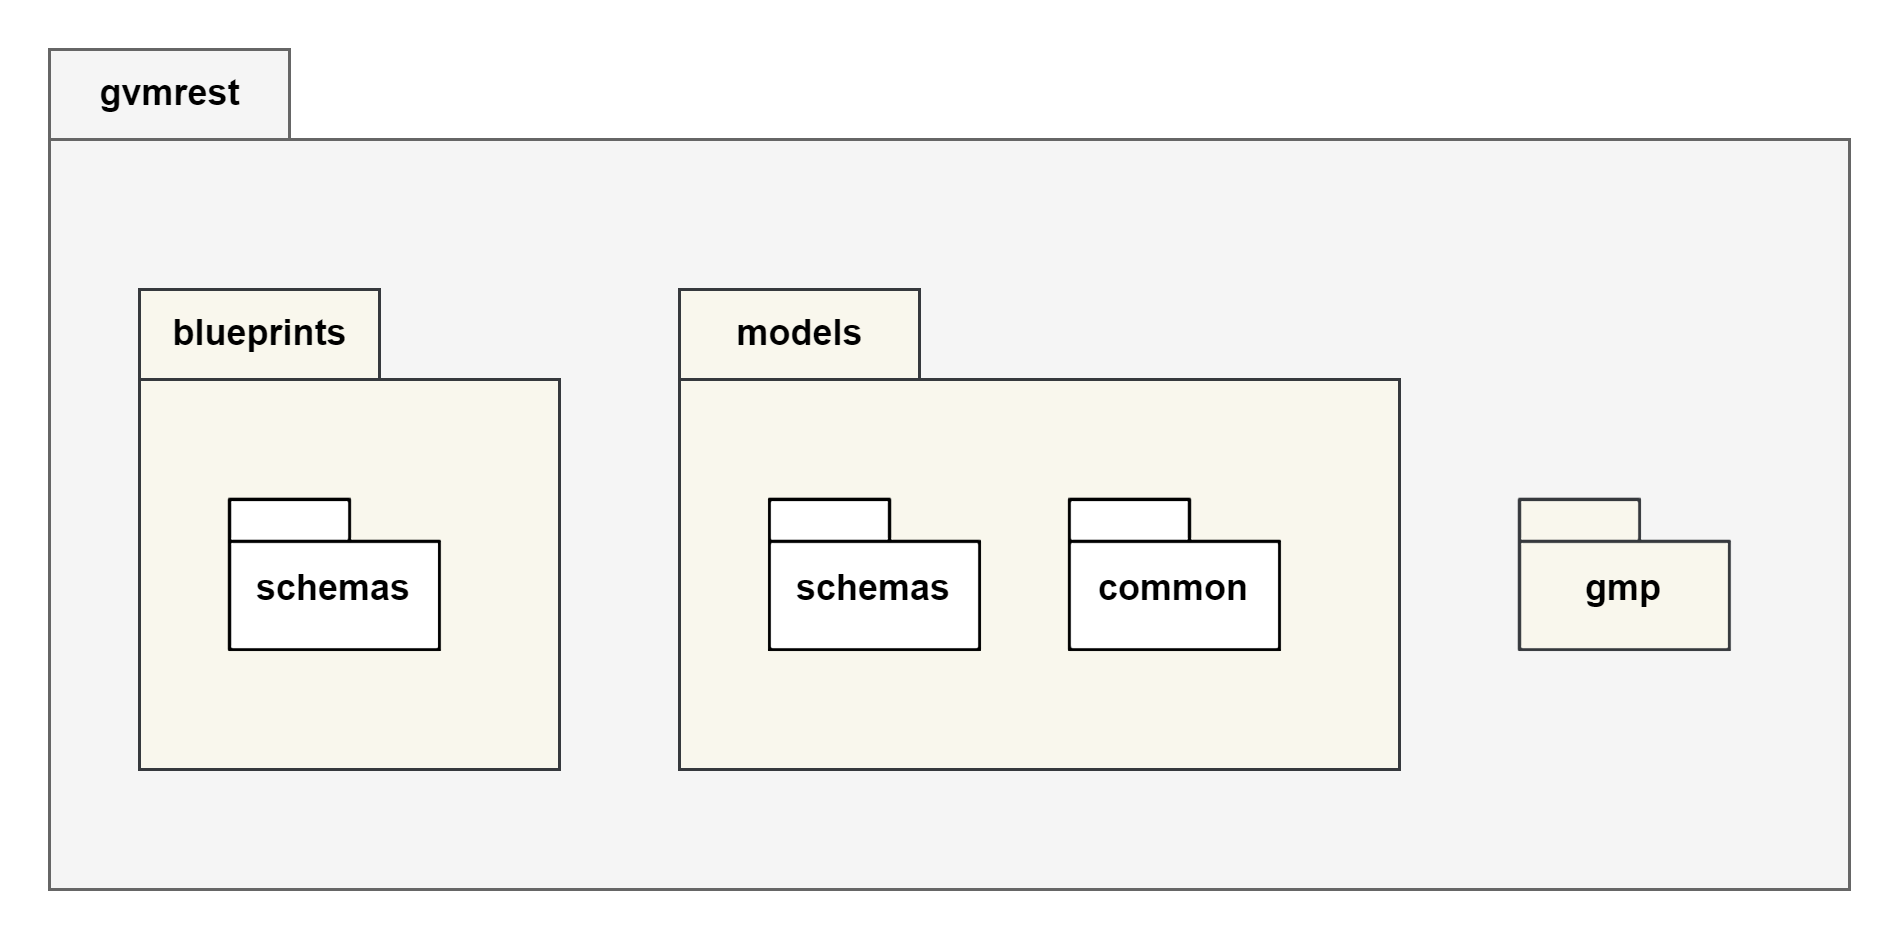
\includegraphics[width=0.8\textwidth]{img/packages.png}
    \caption{Diagramma dei package del backend Flask}
\end{figure}

\subsection{File di inizializzazione}
I file \texttt{\_\_init\_\_.py} di alcuni di questi package sono stati utilizzati in modo peculiare per ottimizzare la configurazione dell'applicazione:
\begin{itemize}
    \item Nel package principale \texttt{gvmrest} il file di \emph{init} implementa un'\emph{application factory} (o \emph{factory function}), un design pattern comune nei progetti Flask.

\begin{figure}
\begin{pycode}
def create_app():
    app = APIFlask(__name__)
    env = DotEnv(app)
    env.init_app(app)
    app.security_schemes = {
        'cookie': {
            'type': 'apiKey',
            'in': 'cookie',
            'name': 'session'
        }
    }
    app.config.from_mapping(
        SESSION_COOKIE_HTTPONLY=True,
        REMEMBER_COOKIE_HTTPONLY=True,
        SESSION_COOKIE_SAMESITE='Strict'
    )

    setup_server_side_sessions(app)

    from gvmrest import blueprints
    blueprints.register_into(app)

    CSRFProtect(app)

    setup_cors(app)

    return app
\end{pycode}
\caption{Application factory}
\end{figure}

    \item Nel package di secondo livello, \texttt{blueprints}, l'inizializzazione contiene una funzione dedicata alla registrazione di tutti i Blueprint Flask contenuti nel package. Questo approccio consente all'\emph{application factory} di richiamare semplicemente questa funzione, evitando la necessità di enumerare singolarmente tutti i blueprint.

\begin{figure}
\begin{pycode}
API_PREFIX = '/api'

def register_into(app: APIFlask):
    from .auth import bp, login_manager
    app.register_blueprint(bp, url_prefix=API_PREFIX + bp.url_prefix)
    login_manager.init_app(app)
    
    from .configs import bp
    app.register_blueprint(bp, url_prefix=API_PREFIX + bp.url_prefix)
    
    from .scanners import bp
    app.register_blueprint(bp, url_prefix=API_PREFIX + bp.url_prefix)

    ...
\end{pycode}
\caption{Registrazione dei blueprint}
\end{figure}
    
    In questo modo, il punto di variabilità si concentra esclusivamente nel file \texttt{\_\_init\_\_.py} del package, semplificando la manutenibilità e rendendo più agevole l'aggiunta o la rimozione di blueprint in futuro.
\end{itemize}

\subsection{Blueprint, REST API e MethodView}
L'uso di APIFlask implica la necessità di usare i Blueprint forniti dalla libreria, che sono di fatto un \emph{wrapper} attorno ai Blueprint Flask (chiamati \texttt{APIBlueprint}).

Per strutturare ancora di più il codice, si è cercato di fornire un'architettura similare a tutti i Blueprint dedicati a compiti simili. Infatti, quasi tutti i blueprint effettuano le classiche operazioni CRUD\footnote{Create, Read, Update, Delete: ovvero creare una risorsa, leggere una risorsa, aggiornare una risorsa, cancellare una risorsa} con vari gradi di completezza.

Flask mette a disposizione la classe \texttt{MethodView} proprio per questo caso. Si tratta di una classe che consente di gestire più metodi HTTP (ad esempio GET, POST, PUT, DELETE) all'interno di una singola classe. Ciò consente di organizzare il codice in modo più pulito e facile da mantenere.

Le MethodView sono utili quando si desidera gestire più azioni su una stessa risorsa in modo semantico (caratteristica chiave delle REST API), ad esempio:
\begin{itemize}
    \item Gestire una richiesta GET per recuperare i dati di una risorsa
    \item Gestire una richiesta POST per creare una nuova risorsa
    \item Gestire una richiesta PUT per aggiornare una risorsa esistente
    \item Gestire una richiesta DELETE per eliminare una risorsa
\end{itemize}

\begin{figure}
\begin{pycode}
bp = APIBlueprint('users', __name__, url_prefix='/users')

class Users(MethodView):
    decorators = [login_required, bp.doc(security='cookie')]
    
    @bp.input(PaginatedUsersQuery, location='query')
    @bp.output(PaginatedUsers)
    def get(self, query_data: dict):
        data, total, pages = models.User.paginate(
            page=query_data['page'],
            filter_string='',
            sort=query_data['sort'],
            direction=query_data['direction']
        )
    
        return {
            'total': total,
            'page': query_data['page'],
            'pages': pages,
            'data': data
        }
    
    @bp.input(UserStoreRequest, arg_name='user')
    @bp.output(UserSchema, status_code=201)
    def post(self, user: dict):
        try:
            return models.User.create(user).__dict__, 201
        except GvmResponseError as e:
            return {
                'message': e.message
            }, int(e.status)
    
    
class User(MethodView):
    decorators = [login_required, bp.doc(security='cookie')]
    
    @bp.output(UserSchema)
    def get(self, user_uuid):
        try:
            return models.User.find(user_uuid).with_tasks()
        except GvmResponseError as e:
            return {'message': e.message}, int(e.status)
    
    ...

bp.add_url_rule('', view_func=Users.as_view('users'))
bp.add_url_rule('/<uuid:user_uuid>', view_func=User.as_view('user'))
\end{pycode}
\caption{Blueprint API e MethodView con decoratori comuni}
\end{figure}

Le MethodView consentono anche di applicare globalmente i decoratori Python, definendoli come attributi d'istanza. Nel caso specifico, le nostre MethodView sono definite con i decoratori di Flask-Login, rendendo tutte le viste automaticamente protette dall'accesso non precedentemente autorizzato. Inoltre, con un ulteriore decoratore proprio di APIFlask è possibile segnalare le viste come protette dall'autenticazione, ottenendo questa informazione durante la generazione automatica della documentazione interattiva.

\subsection{Schemi Marshmallow}
Dalla scelta di utilizzare il meta-framework di APIFlask deriva anche la scelta obbligata della libreria di gestione degli schemi dei dati: Marshmallow (invece di Pydantic). APIFlask supporta di fatto solo Marshmallow, il che ha reso questa libreria una scelta naturale, anticipata già in \ref{design-marshmallow}.

Marshmallow si integra facilmente con Flask tramite appositi plugin, ma APIFlask offre una serie di automazioni che semplificano la validazione degli schemi in input (JSON) e l'auto-formattazione delle entità restituite in JSON. Queste automazioni includono il filtraggio e il parsing degli attributi sia in input che in output, permettendo conversioni basilari e avanzate, con la possibilità di utilizzare callback e hook astratti offerti dalle classi base di Marshmallow e personalizzabili nelle singole classi di schema attraverso override.

\begin{figure}
\begin{pycode}
def unique_username(username: str):
    response = g.gmp.get_users(filter_string=f'name={username}')
    if response.find('user') is not None:
        raise ValidationError('Username already exists')


class UserStoreRequest(Schema):
    name = fields.String(
        required=True,
        validate=[
            validators.Length(min=1, error='Please supply a name'),
            unique_username
        ]
    )
    password = fields.String(
        required=True,
        validate=validators.Length(min=1, error='Please supply a password')
    )
    role = fields.String(
        required=True,
        validate=validators.OneOf(['user', 'tenant'])
    )
    quota_id = fields.UUID(required=True)
    hosts = fields.String(load_default='',
                          example='192.168.1.42,192.168.1.200-220,a.com',
                          validate=validate_hosts_specification)
    hosts_allow = fields.Boolean(default=False)

    @post_load
    def split_hosts(self, data, **kwargs):
        data['hosts'] = [host for host in data['hosts'].split(',') if host != '']
        data['role'] = current_app.config.get(f"ROLE_{data['role'].upper()}")
        return data
\end{pycode}
\caption{Esempio di schema Marshmallow usato per validare le richieste in ingresso}
\end{figure}

Tuttavia, a differenza di Pydantic, Marshmallow non consente di utilizzare direttamente i tipi nativi di Python, ma richiede l'uso di classi wrapper specifiche della libreria. Questo introduce un certo livello di astrazione indesiderata, anche se i vantaggi dall'uso di Marshmallow superano gli svantaggi che porta il non usare una libreria di questo tipo.

Per ogni entità, è necessario definire uno schema Marshmallow. Questi schemi sono stati organizzati in file separati, tipicamente uno schema per file.

I file di schema sono stati raggruppati in due package \texttt{schemas/}, che si trovano sotto \texttt{models/} (dove sono specificate le entità e i modelli di business logic) e \texttt{blueprints/} (dove sono definiti i formati delle richieste API, che spesso sono lievemente diversi o semplificati rispetto ai dati reali, e delle risposte API, che possono utilizzare la paginazione e avvolgere i dati di base, rendendo insufficiente lo schema della singola entità in alcuni casi).

\section{ORM basato su GMP}
Una parte importante dello sviluppo è stata la creazione di un \textbf{ORM (Object-Relational Mapping)} basato sull'API di GMP.

\subsection{Razionale}
Un \textbf{ORM} è una tecnica che consente di interagire con un database utilizzando oggetti di programmazione, piuttosto che scrivere direttamente query SQL. Questo approccio semplifica la gestione dei dati, permettendo agli sviluppatori di lavorare con le entità come se fossero oggetti, senza doversi preoccupare della complessità delle operazioni di database sottostanti.

Nel nostro caso, la libreria \texttt{python-gvm} restituisce entità in formato XML, che alla fine è essenzialmente puro testo / stringa di caratteri. Per tradurre queste entità in JSON, è necessario effettuare un parsing. Tuttavia, una semplice conversione da XML in oggetti JSON non è sufficiente, poiché il servizio Python deve anche eseguire query sulle entità correlate fra loro da relazioni (ad es. come reperire i report generati da un task di scansione specifico). Per fare questo occorre che le entità siano in qualche modo ``intelligenti'', e una rappresentazione ``stupida'' di tipo testuale è scomoda oltre che inefficiente.

Stante così le cose si può comunque costruire direttamente le query al sistema Greenbone utilizzando il linguaggio Powerfilter descritto in \ref{powerfilter} (in questo contesto Powerfilter rappresenta in tutto e per tutto il linguaggio SQL). Tuttavia, questo approccio comporterebbe un'interazione diretta con il livello più basso, con i controller del pattern MVC (i blueprint Flask, in questo caso) che dovrebbero gestire direttamente la logica dell'applicazione. È preferibile mantenere questa logica all'interno dei modelli, che sono stati progettati proprio per questo scopo.

Le classi di modello implementano di conseguenza un ORM atipico e unico nel suo genere. Di solito, un ORM si interfaccia direttamente con un'istanza di database, solitamente usando internamente il linguaggio SQL; ma, nel nostro caso, l'ORM si connette invece a un database indirettamente esposto tramite un'API pubblicata su Socket UNIX (GMP e il linguaggio di query Powerfilter).

\subsection{Implementazione concreta}
In questo ORM ogni sua classe modello è creata a partire dal documento XML reperito da GMP, che rappresenta un numero qualsiasi di entità reperite dal sistema.

Questo documento XML ritornato dalla libreria è già un oggetto Python (un'istanza di \texttt{Element} della dipendenza \texttt{lxml}) che facilita il parsing e l'estrazione dei dati. In sostanza, questo oggetto rappresenta il documento in RAM, consentendo delle operazioni di ricerca e manipolazione giusto un po' più comode rispetto alla cruda manipolazione di testo. Tuttavia, questa flessibilità non è sufficiente e la rappresentazione è troppo semplice per i nostri scopi.

Ogni classe dell'ORM agisce nel medesimo modo: il costruttore della classe modello estrae il contenuto del documento XML utilizzando semplici query ai tag del documento (con l'API di \texttt{lxml}), sfruttando metodi nativi o interfacce XPath\footnote{XPath è un linguaggio di query avanzato utilizzato per navigare attraverso gli elementi e gli attributi di un documento XML, secondo logiche complesse e permettendo di selezionare nodi specifici in modo altamente flessibile ed efficiente.}.

\begin{figure}
\begin{pycode}
class User(Authenticable):
    id: uuid.UUID
    name: str
    role_id: uuid.UUID
    role: str
    comment: str
    created: str
    owner: str
    hosts: dict
    quota: dict
    tags: list[Tag]
    in_use: bool

    def __init__(self, get_users_response: etree.Element):
        self.tasks = []
        user_tag = get_users_response.find('user')
        self.id = user_tag.attrib['id']
        self.name = user_tag.find('name').text
        self.role_id = user_tag.find('role').attrib['id']
        self.role = self._role_human(self.role_id)
        self.comment = user_tag.find('comment').text
        self.created = user_tag.find('creation_time').text
        self.owner = user_tag.find('owner/name').text
        self.hosts = {
            'allow': not bool(int(user_tag.find('hosts').attrib['allow'])),
            'exclusions': user_tag.find('hosts').text
        }
        self.in_use = bool(int(user_tag.find('in_use').text))

        tags = get_users_response.find('user/user_tags')
        tags = [] if tags is None else tags.xpath('tag')
        self.tags = [Tag(tag) for tag in tags]

        self.quota = self.get_month_quota()
    
    ...
\end{pycode}
\caption{Destrutturazione dal documento XML a Python}
\end{figure}

Questa procedura consente di realizzare una prima traduzione da XML a un oggetto Python specifico per l'entità rappresentata (\texttt{Task}, \texttt{Report}, eccetera). A questo punto, ogni classe può offrire metodi specifici che astraggono l'interazione con le altre entità e, indirettamente, con il database. Di fatto si crea un ORM, ma astraendo qualcosa di più specialistico rispetto al più comune caso di un database SQL direttamente controllato da noi.

In questo modo, i controller (blueprint nel nostro caso) rimangono snelli e focalizzati, mentre il codice di basso livello e l'accesso ai dati sono segregati nei modelli e organizzati in metodi separati. Questo approccio per quanto inusuale aumenta la coerenza e riduce l'accoppiamento, migliorando in modo decisivo la manutenibilità e la chiarezza del codice. Non solo, la separazione del codice di accesso ai dati in metodi distanti favorisce e incoraggia anche un riuso del codice che non sarebbe altresì possibile.

\subsection{API generica / paginazione}
Nell'implementazione dell'ORM, sono stati creati metodi generici per facilitare la frequente interazione con le entità restituite dalla API GMP. Poiché queste entità sono quasi sempre restituite paginate in partenza, è fondamentale gestire la paginazione a livello di superclasse.

La classe \texttt{Model}, che funge da superclasse per tutte le classi di modello, implementa due metodi principali per l'interazione con il database:
\begin{itemize}
    \item \texttt{all()}: questo metodo restituisce tutti i record di un determinato modello, ``paginati'' di default, insieme al numero totale di record disponibili (non solo quelli nella pagina corrente). \texttt{all()} accetta anche una \texttt{filter\_string} definita in Powerfilter, che gestisce effettivamente la paginazione. È decorato come \texttt{@abstractmethod}, il che significa che l'implementazione specifica deve essere fornita dalle sottoclassi concrete. Tuttavia, l'idea è che \texttt{all()} non venga utilizzato direttamente, ma solo attraverso l'altro metodo di questa classe.
    \item \texttt{paginate()}: Questo metodo concreto riceve tutti i parametri relativi alla paginazione, come il numero di pagina, il numero di oggetti per pagina, l'ordinamento (ascendente o discendente e su quale attributo) e il filtraggio (gestito tramite una \texttt{filter\_string} in Powerfilter). \texttt{paginate()} esegue i calcoli necessari per determinare la pagina e costruisce una nuova \texttt{filter\_string} decorando quella iniziale con i valori necessari per gestire la paginazione. Questa \texttt{filter\_string} viene poi passata a \texttt{all()}, che recupera i record appropriati. Il metodo \texttt{paginate()} restituisce quindi i record paginati, insieme a informazioni utili per il frontend, come il numero totale di pagine e il numero totale di record.
\end{itemize}

\begin{figure}
\begin{pycode}
class Model:
    def __repr__(self):
        import pprint
        return pprint.pformat(self.__dict__)

    @classmethod
    def paginate(cls,
                 page: int,
                 filter_string: str,
                 rows: int = 20,
                 sort: str = None,
                 direction: str = 'asc'
                 ) -> tuple[list['Model'], int, int]:

        first = (page - 1) * rows + 1

        sort_kw = 'sort' if direction == 'asc' else 'sort-reverse'
        sort_query = None if sort is None else f'{sort_kw}={sort}'
        filter_string = filter_string + f" first={first} rows={rows} " + sort_query

        models, total = cls.all(filter_string=filter_string)

        pages = math.ceil(total / rows)

        return (
            models,
            total,
            pages
        )

    @classmethod
    @abstractmethod
    def all(cls, filter_string: str) -> tuple[list['Model'], int]:
        pass
\end{pycode}
\caption{Modello base dell'ORM basato su GMP}
\end{figure}

Inoltre, la classe \texttt{Model} implementa anche il \emph{magic method} \texttt{\_\_repr\_\_()}, fornendo un'implementazione di default per la stampa in ambiente CLI. In particolare, l'implementazione usa \texttt{pprint} per stampare la rappresentazione interna a dizionario dell'oggetto, risultando particolarmente utile durante il debug o i test.

Per gestire la definizione di classi e metodi astratti, è stata necessariamente utilizzata la libreria \textbf{ABC (Abstract Base Classes)} di Python\footnote{Python non supporta le classi astratte a livello di linguaggio.}. Questa libreria consente di definire classi base astratte e metodi astratti, fornendo un modo per garantire che le sottoclassi implementino determinati metodi, mantenendo così una struttura coerente nell'ORM.

\subsection{Deserializzazione}
Il processo di deserializzazione da XML a oggetto Python inizia quando i costruttori delle classi modello ricevono un'istanza del documento XML in memoria, che, come già detto poco sopra, viene decomposto in attributi d'istanza del nuovo oggetto, convertendo i valori estratti in una rappresentazione nativa di Python.

I valori ovviamente necessitano di \emph{casting}, siccome la rappresentazione XML è puramente testuale, ma anche di una gestione del valor nullo e dell'assenza di valore. È comune infatti che alcuni valori siano del tutto assenti nel documento XML. In questi casi, si considera il tipo di riferimento come \emph{nullable}, utilizzando un tipo unione con il \texttt{None} di Python. Questo approccio consente di gestire in modo efficace i dati incompleti, dichiarando nell'interfaccia il rischio di inconsistenza, similarmente all'approccio usato da linguaggi come TypeScript o Kotlin. Questo viene fatto mediante le \texttt{type hint}, largamente usate in questo progetto. Questo non solo aiuta a mediare la natura dinamica di Python, ma fornisce anche un supporto migliore per le funzionalità di autocomplete negli IDE.

In generale, le classi concrete che rappresentano i modelli sono simili a una \emph{dataclass} di Python, poiché si concentrano principalmente sulla memorizzazione dei dati. Tuttavia, alcune di queste classi esibiscono anche comportamenti più ricchi grazie all'aggiunta di metodi specifici, che permettono di eseguire operazioni più complesse o di interagire con altre entità in modo meno ripetitivo e ridondante.

\subsection{Serializzazione}
Quando gli oggetti devono essere restituiti nella risposta della API, questi vengono semplicemente restituiti così come sono, senza nessuna particolare operazione. La presenza dei valori negli attributi della classe e lo schema Marshmallow fa sì che il processo di serializzazione sia assolutamente automatico, con lo schema Marshmallow che specifica cosa viene fatto passare della classe e secondo quale formato\footnote{Si noti che lo standard JSON non supporta numeri decimali, che vengono quindi restituiti come stringhe di caratteri. La conversione verrà gestita dal frontend.}.

\section{Quality of Detection}
Pur essendo un attributo specifico di OpenVAS si è voluto inserire comunque il QoD (già descritto precedentemente in \ref{qod}) nell'interfaccia dell'API, anticipando un eventuale parametro generico che identifichi l'affidabilità dei risultati, indipendente dal backend di scansione.

Questo parametro viene fornito all'API in tutte le richieste di risorse con paginazione, che di fatto sono le uniche che possono usare il valore di QoD per filtrare i risultati.

\section{Gestione delle schedule}
Le schedule sono gestite internamente da OpenVAS come delle stringhe in formato iCalendar, più alcuni metadati usati per la loro identificazione.

\subsection{iCalendar}
\textbf{iCalendar} è un formato standard per la rappresentazione di informazioni relative a eventi, appuntamenti e attività. È utilizzato per scambiare dati di calendario tra diverse applicazioni e servizi. Il formato è definito nella specifica RFC 5545 \cite{rfc5545} e consente di creare file con estensione \texttt{.ics}, che possono contenere dettagli come:
\begin{itemize}
    \item Data e ora di inizio e fine di un evento
    \item Fuso orario
    \item Descrizione dell'evento
    \item Luogo
    \item Informazioni di contatto
    \item Ripetizioni (per eventi ricorrenti)
    \item Allerta e promemoria
\end{itemize}
Questo formato è utile anche per specificare calendari che possono essere importati o condivisi tramite applicazioni come Outlook, Google Calendar o altre.

Per quanto riguarda il caso in esame, OpenVAS si serve di questo formato esclusivamente per specificare le scansioni che devono essere fatte in accordo con la schedule in oggetto, di fatto limitandosi alle seguenti informazioni:
\begin{itemize}
    \item Data e ora di inizio e fine scansione
    \item Ripetizioni per eventi ricorrenti
    \item Fuso orario
\end{itemize}

L'uso di un formato standard ovviamente semplifica lo sviluppo poiché ci si può appoggiare a librerie che automatizzano il processo di parsing e generazione di stringhe aderenti al formato iCalendar. Addirittura la documentazione stessa di \texttt{python-gvm} suggerisce l'uso della libreria \texttt{icalendar} di Python, e così si è fatto nel progetto in esame.

\begin{figure}
\begin{pycode}
icaltext = schedule_xml.find('icalendar').text
cal = Calendar()
self._ical = cal.from_ical(icaltext)
subcomp = self._ical.subcomponents[1]
dt_from: datetime.datetime = subcomp['dtstart'].dt
self.start = dt_from.isoformat()
self.duration = subcomp['duration'].dt.total_seconds()
self.dtstamp = subcomp['dtstamp'].dt.isoformat()
self.freq = subcomp['rrule']['freq'][0] if 'rrule' in subcomp else 'ONCE'
\end{pycode}
\caption{Uso di \texttt{icalender}}
\end{figure}

L'uso dello standard iCalendar è tornato utile anche in fase di standardizzazione dell'interfaccia dei dati in uscita, mantenendo il formato delle \texttt{RRULE} di iCalendar per descrivere il tipo di ricorrenza delle schedule.

\section{Autenticazione}
\subsection{Autenticazione con l'API Flask}
L'autenticazione degli utenti nell'API Flask è gestita utilizzando \textbf{Flask-Login}, una delle librerie più affidabili e popolari dell'ecosistema Flask. Questa libreria semplifica notevolmente il processo di autenticazione, implementando un sistema basato su cookie per gestire le sessioni degli utenti.

Flask-Login automatizza gran parte delle operazioni di login e logout, fornendo metodi semplici e intuitivi per eseguire queste funzioni quando necessario. Inoltre, la libreria offre un decoratore \texttt{@login\_required}, che consente di proteggere immediatamente e facilmente qualsiasi metodo-vista di Flask, garantendo che solo gli utenti autenticati possano accedervi.

Un aspetto fondamentale di Flask-Login è la necessità di fornire un metodo che restituisca l'oggetto utente corrispondente a un identificativo specifico. Questo metodo deve restituire l'oggetto utente se l'identificativo è valido, oppure None se non lo è. L'identificativo utilizzato è a discrezione del programmatore, così come la classe utente, purché vi sia coerenza interna nel sistema.

Nel contesto di questo progetto, è stato scelto di utilizzare l'ID dell'utente fornito dall'API GMP come identificativo. Questo ID è un UUID, in linea con il formato utilizzato per tutte le altre risorse interne al sistema GVM. Per rappresentare l'utente, è stata utilizzata la classe di modello che corrisponde alla risorsa utente di GMP, garantendo così una gestione coerente e integrata delle informazioni relative agli utenti.

\begin{figure}
\begin{pycode}
login_manager = LoginManager()

@login_manager.user_loader
def load_user(user_id: str):
    gmp = get_gmp()
    if gmp is None:
        return None
    res = gmp.get_user(user_id)
    return User(res)
\end{pycode}
\caption{User loader di Flask-Login}
\end{figure}

\subsection{Autenticazione con l'API GMP}
L'autenticazione dell'applicazione Flask con l'API sottostante di GMP ha rappresentato invece una sfida complessa e delicata, come quasi tutti i casi in cui un'applicazione deve interagire in modo sicuro con un sistema di terze parti che non è ben configurato in tal senso (ad esempio, supportando OAuth).

Segue un'analisi delle problematiche riscontrate e dell'analisi effettuata di varie soluzioni applicative prima di giungere alla soluzione che è stata effettivamente adottata nel progetto.

\subsubsection{Requisiti}
Innanzitutto, si vuole che la sessione dell'utente loggato mantenga una connessione con l'API di GMP in background. Ma questo non è un compito banale. Le connessioni HTTP sono, per loro natura, \emph{stateless}, mentre l'API di GMP opera su una socket UNIX, che è intrinsecamente \emph{stateful} rispetto alle richieste HTTP in arrivo.

La connessione con l'API di GMP viene stabilita aprendo una socket UNIX e fornendo immediatamente le credenziali dell'utente, ovvero nome utente e password. Questo approccio consente di eseguire tutte le operazioni successive con i privilegi dell'utente autenticato.

\subsubsection{Pooling di connessioni}
Una possibilità può essere mantenere viva questa connessione in memoria tra le chiamate HTTP; ma questo è problematico, poiché i server web operano in modalità di parallelismo. Ad esempio, Gunicorn, il server web utilizzato per il deployment, gestisce le richieste in ingresso creando una serie di processi \emph{worker}, i quali non condividono la memoria RAM. Di conseguenza, mantenere le connessioni alla socket in memoria porterebbe a errori di tipo \emph{time-dependent}: una richiesta potrebbe avere successo solo se viene gestita da quel particolare \emph{worker} che ha tenuto in memoria la connessione, altrimenti fallirebbe.

\subsubsection{Multiprocessing / multithreading}
Sebbene Gunicorn consenta di precaricare un pezzo di codice e di fare il \emph{fork} dei processi worker successivamente, questo approccio garantisce solo che il pool di connessioni parta dallo stesso stato iniziale, senza assicurare coerenza nelle operazioni successive. Un'alternativa sarebbe implementare soluzioni di multiprocessing o multithreading. Tuttavia, il multiprocessing richiede lo scambio di messaggi e strutture dati tra processi, e le connessioni a socket UNIX non sono facilmente serializzabili con nessuna delle strategie di \emph{marshalling} comuni nell'ecosistema Python.

D'altra parte, il multithreading richiederebbe di configurare i worker di Gunicorn con GEvent, trasformando il server web in un singolo processo con più thread. Questo approccio, però, introduce la necessità di gestire sezioni critiche (per la gestione del pool delle connessioni) e meccanismi di sincronizzazione, come i semafori, di fatto compromettendo le performance. Tuttavia, ciò comporta un ulteriore problema: una singola connessione UNIX non può essere "multiplexata" e può rispondere a un solo comando alla volta. Anche con l'implementazione di sezioni critiche e semafori, le richieste simultanee sarebbero ingestibili.

\subsubsection{Gestione delle credenziali di terze parti}
In sintesi, l'unica soluzione praticabile per evitare di richiedere all'utente di inserire nome utente e password ad ogni chiamata API (un approccio di fatto estremamente scomodo e impraticabile) è quella di memorizzare in RAM il nome utente e, purtroppo, la password. Questo consente di ricreare le connessioni con la socket UNIX per ogni chiamata, garantendo la massima performance e soprattutto, scongiurando problemi di consistenza dei dati o dipendenze dalla rete, che sarebbero altresì inevitabili.

Questo approccio, per quanto sub-ottimo dal punto di vista delle buone pratiche di security, come si è visto è di fatto necessario per realizzare il sistema in oggetto.

Per mitigare il più possibile questa soluzione si sono introdotti tutta una serie di accorgimenti:
\begin{itemize}
    \item Le credenziali di terze parti sono salvate in sessione, ma rese \emph{server-side} rispetto al default \emph{client-side} di Flask.
    \item Le sessioni \emph{server-side} sono salvate in un'istanza di Redis, resa accessibile solo dalla rete interna di Docker Compose ed è pertanto inaccessibile da al di fuori della macchina. Internamente alla macchina invece è necessario disporre dei permessi di \texttt{root} per accedervi.
    \item Un'istanza di \textbf{Fernet} è generata e condivisa tra tutti i processi mediante il precaricamento di Gunicorn, efficace in questo caso visto che l'istanza non cambia nel tempo. Fernet è un sistema di crittografia simmetrica che fa parte della libreria di crittografia \texttt{cryptography} in Python, e di fatto implementa AES in modalità CBC.
    
    Grazie a Fernet le password sono crittografate prima di essere salvate su Redis. Chiaramente è meno sicuro di un hash, ma le hash impediscono il recupero della password che in questo caso è purtroppo necessario.
    \item La password usata da AES è generata casualmente al momento della creazione del server Gunicorn e non è mai salvata su disco o stampata a schermo, di fatto rimanendo solo nella RAM della macchina. Questo significa che ad ogni riavvio del server la password è scelta di nuovo e sessioni esistenti diventano invalidate.
\end{itemize}

\subsection{Proxying dell'API GMP}
Flask supporta l'uso di un oggetto ``globale'' per tutta la durata della richiesta web, chiamato semplicemente \texttt{g}. Questo oggetto è usato per riferirsi alla connessione con l'API GMP (in un'applicazione web maggiormente classica conterrebbe probabilmente un riferimento alla connessione con il database SQL), usando un metodo \texttt{get\_gmp()} che di fatto implementa un design pattern di tipo \emph{Proxy}.

\begin{figure}
\begin{pycode}
def get_gmp() -> None | GMPv224[Any] | GMPv225[Any]:
    if 'gmp' not in g:
        g.gmp = Gmp(
            connection=UnixSocketConnection(path=current_app.config.get('GVMD_SOCKFILE')),
            transform=EtreeCheckCommandTransform()
        ).__enter__()
        try:
            g.gmp.authenticate(
                fernet.decrypt(session['name']).decode(),
                fernet.decrypt(session['password']).decode()
            )
        except InvalidToken as _:
            return None

    return g.gmp
\end{pycode}
\caption{Metodo proxy per la connessione GMP}
\end{figure}

Nello specifico, quando questo metodo viene invocato esso verifica se l'istanza di GMP è già presente, ovvero, se la connessione è stata già stabilita:
\begin{itemize}
    \item Se sì, ritorna la connessione già stabilita.
    \item In caso contrario è necessario stabilire una nuova connessione. La libreria \texttt{python-gvm} è usata per connettersi alla socket UNIX. Quindi, vengono reperite dalla sessione Redis le credenziali dell'utente, decriptate e infine usate per autenticare la connessione.
\end{itemize}

Infine, quando il flusso di richiesta / risposta web si conclude l'istanza Flask chiude la connessione manualmente, siccome (come già detto precedentemente) non è possibile fare \emph{pooling} di queste connessioni per ottimizzare le risorse del server.

\begin{figure}
\begin{pycode}
def close_gmp(e=None):
    gmp = g.pop('gmp', None)

    if gmp is not None:
        gmp.__exit__(None, None, None)
\end{pycode}
\caption{Metodo di chiusura delle connessioni GMP}
\end{figure}

\begin{figure}
\begin{pycode}
from .gmp import close_gmp
app.teardown_appcontext(close_gmp)
\end{pycode}
\caption{Aggancio per chiudere le connessioni}
\end{figure}

\section{Quota di scansione}
\subsection{Definizione del valore massimo}
La quota di scansione come detto è stata gestita mediante il sistema di tagging interno a Greenbone. In particolare, ogni utente riceve un tag di nome \texttt{quota:total} con come valore il numero di scansioni massime consentite per ogni mese. Questo tag è specificato al momento della creazione dell'utente da parte dell'utenza di livello superiore.

\subsection{Calcolo della quota consumata}

\begin{figure}
\begin{pycode}
def get_consumed_quota(self, at: datetime):
    next_month = at + relativedelta(months=1)

    self.hosts_for_target = {}
    targets, _ = Target.all(filter_string=f'owner={self.name}')
    for target in targets:
        self.hosts_for_target[target.id] = target.max_hosts

    total_hosts = self.sum_past_reports_consumption(at, next_month)
    total_hosts += self.sum_scheduled_tasks_consumption()

    return total_hosts
\end{pycode}
\caption{Calcolo della quota consumata (ad alto livello)}
\end{figure}

La quota consumata è calcolata sommando i contributi di due parti:
\begin{itemize}
    \item Le scansioni passate in questo mese, usando i report delle scansioni\footnote{Per tenere sotto controllo l'occupazione del disco i report sono cancellati a rotazione. Ovviamente, il valore di \emph{turnaround} è stato scelto in modo tale da non compromettere la correttezza del precedente calcolo.} per determinare il numero di host coinvolti ogni volta (che non dipende da quanti host fossero attivi o meno al momento della scansione).
    \item Le scansioni future di questo mese, ovvero quelle pianificate / ricorrenti. Queste sono determinate con l'uso di una libreria Python specializzata, \texttt{recurring\_ical\_events}, che garantisce una gestione facilitata degli eventi ricorrenti definiti con standard iCalendar. Non avendo ancora rapporti, per contare l'impatto della scansione della quota si usa il bersaglio configurato.
\end{itemize}
Questa quota è quindi definita come attributo d'istanza dell'utente.

\subsection{Controllo della quota consumata}
La quota è controllata al momento dell'aggiunta di un task di scansione. In particolare, nel backend è stato definito un endpoint che verifica se il task passato nella richiesta API è accettabile per la quota fornita, oppure no. Per farlo opera in modo diverso a seconda del task specificato:
\begin{itemize}
    \item Se il task è configurato per l'esecuzione immediata allora questo è controllato esclusivamente rispetto alla quota disponibile di questo mese.
    \item Se invece il task è configurato per un esecuzione periodica allora la quota è controllata per ogni mese futuro, fermando i controlli con un'orizzonte temporale di un anno dal momento della creazione.
\end{itemize}
In questo modo la quota valida è controllata a monte dell'unica operazione che può intaccarla, così da garantirne sempre la consistenza.

Si noti che di fatto il sistema OpenVAS consente tranquillamente la definizione di un qualsivoglia numero di scansioni, senza rispettare i valori specificati nei tag. L'API wrapper fatta con Flask è quella che impone il controllo a livello applicativo della validità delle operazioni proposte dall'utente.

\section{Multi-tenancy}
\label{roles}
La multi-tenancy è stata gestita usando il sistema dei ruoli nativo di Greenbone:
\begin{itemize}
    \item \textbf{1° livello / Super amministratore}: per questo ruolo è stato usato il ruolo di \textbf{Super Admin}, già incluso nel sistema Greenbone. Tale ruolo va necessariamente creato da linea di comando interagendo direttamente con il demone \texttt{gvmd}. Inoltre, l'utente di super amministratore è impostata come proprietario degli oggetti reperiti dal \emph{feed} di Greenbone.

    Ci può essere un solo utente sotto questo ruolo, che di fatto può fare e vedere ogni cosa rispetto ad ogni entità del sistema.
    \item \textbf{2° livello / Tenant}: per questo ruolo è stato usato il ruolo di \textbf{Admin}, già incluso nel sistema Greenbone.

    Inoltre, serve aggiungere i permessi per la lettura e la modifica\footnote{In questo contesto la modifica dei tag consente l'assegnamento dei tag.} dei tag di quota.
    \item \textbf{3° livello / Utente finale}: infine, per l'ultimo livello della gerarchia è stato usato un ruolo personalizzato. Infatti, il ruolo \textbf{User} offerto dal sistema di ruoli nativo di Greenbone è insufficiente, non consentendo i permessi di lettura sugli utenti\footnote{In linea di principio questo non sarebbe un problema, siccome un utente finale del sistema non deve avere modo di vedere gli altri utenti. Tuttavia, il permesso è strutturato in maniera tale che l'utente non può nemmeno vedere sé stesso e questo causa problemi in fase di autenticazione e controllo quota di scansione.}. Di conseguenza, è necessario clonare il ruolo e aggiungere manualmente i permessi di \texttt{get\_users}\footnote{Questo di fatto consente solo la lettura della propria utenza, senza necessità di limitare i permessi appena forniti.}.

    Inoltre, serve aggiungere i permessi per la lettura dei tag di quota.
\end{itemize}
I ruoli così definiti sono usati dal sistema per mezzo dei loro identificativi UUID, forniti tramite il file \texttt{.env}.

Al momento della creazione di un tenant, da parte del super amministratore viene anche creato un gruppo di tenancy denominato sulla base del tenant e in cui il tenant viene automaticamente inserito con permessi di tipo \texttt{Super}\footnote{Ovvero, ha la facoltà di fare e vedere ogni cosa. Di fatto lo si rende un Super Admin localmente alle risorse del gruppo.} e \texttt{modify\_group}\footnote{Per aggiungere risorse al gruppo, come gli utenti che lui crea.}.
    
Inoltre, tutti gli utenti inseriti nel gruppo possono bypassare i permessi di lettura degli utenti per vedere esclusivamente il proprio tenant. Questo è necessario per determinare il proprio gruppo di tenancy e il permesso viene automaticamente creato dal sistema in fase di creazione degli utenti di minor livello.

\begin{figure}
\begin{pycode}
def _create_tenant_group(self):
    group_name = self.get_tenant_group_name()
    res_group = g.gmp.create_group(
        name=group_name,
        comment=f'Created automatically; do not edit manually.'
    )
    group_id = res_group.attrib['id']
    g.gmp.create_permission(
        name='get_users',
        subject_id=group_id,
        subject_type=PermissionSubjectType.GROUP,
        resource_id=self.id,
        resource_type=EntityType.USER,
        comment=f'Created automatically; do not edit manually.'
    )
    g.gmp.create_permission(
        name='Super',
        subject_id=self.id,
        subject_type=PermissionSubjectType.USER,
        resource_id=group_id,
        resource_type=EntityType.GROUP,
        comment=f'Created automatically; do not edit manually.'
    )
    g.gmp.create_permission(
        name='modify_group',
        subject_id=self.id,
        subject_type=PermissionSubjectType.USER,
        resource_id=group_id,
        resource_type=EntityType.GROUP,
        comment=f'Created automatically; do not edit manually.'
    )
\end{pycode}
\caption{Creazione del gruppo di tenancy e dei rispettivi permessi}
\end{figure}

\section{Utilità di testing}
Durante lo sviluppo è stato necessario interagire più volte con l'API GMP per verificare le risposte restituite e testare interattivamente il parsing XML.

Per velocizzare quest'operazione è stata aggiunta direttamente nell'applicazione  un'utilità di testing grazie al framework \textbf{Click}, già integrato con ogni installazione di Flask.

Click è un framework di controllo della riga di comando che consente di creare applicazioni CLI robuste e flessibili. In relazione a Flask, Click è spesso utilizzato per creare comandi CLI personalizzati per le applicazioni Flask, come in questo caso.
Flask fornisce un'integrazione nativa con Click, che consente di creare comandi CLI per eseguire azioni specifiche all'interno dell'applicazione Flask. Ad esempio, è possibile utilizzare Click per creare comandi per inizializzare il database, eseguire test, avviare server di sviluppo, ecc.

In questo caso è stato aggiunto un comando Click (chiamato semplicemente \texttt{gmp}) che una volta invocato dalla linea di comando ci inserisce in una sessione dell'interprete interattivo Python creata appositamente per noi. In questa sessione sono inserite tutte le variabili locali allo \emph{scope} dell'invocazione dell'interprete Python, così da avere a disposizione tutti gli strumenti necessari per testare l'API GMP direttamente dall'interfaccia della libreria di Greenbone:
\begin{itemize}
    \item Una connessione già stabilita e autenticata (se le credenziali sono fornite) con GMP.
    \item Una funzione\footnote{Python consente di definire funzioni locali ad altre funzioni. In questo modo la funzione è disponibile solo nel contesto interattivo creato da Click.} \texttt{pp()} per la stampa a schermo formattata dei documenti XML restituiti dalla API.
\end{itemize}

\begin{figure}
\begin{pycode}
@click.command("gmp")
@click.argument('credentials', required=False)
def test_command(credentials: str):
    def pp(el):
        print(etree.tostring(el, pretty_print=True).decode())

    with Gmp(
        connection=UnixSocketConnection(path=os.getenv('GVMD_SOCKFILE')),
        transform=EtreeCheckCommandTransform()
    ) as gmp:
        if credentials is not None:
            username, password = credentials.split(':')
            gmp.authenticate(username, password)

        import code
        code.interact(local=locals())
\end{pycode}
\caption{Comando Click per testare l'API GMP interattivamente}
\end{figure}

\section{Documentazione API interattiva}
APIFlask include anche una generazione automatica di una documentazione interattiva della API specificata. Questa può essere realizzata in numerosi formati, dal più popolare Swagger fino ad altre varianti.

Questa documentazione permette di testare direttamente nel browser l'API e di consultare a colpo d'occhio:
\begin{itemize}
    \item Endpoint esposti dalla API
    \item Codici di errore e stato HTTP definiti
    \item Schemi dei dati per le richieste e i dati di risposta
\end{itemize}

\begin{figure}
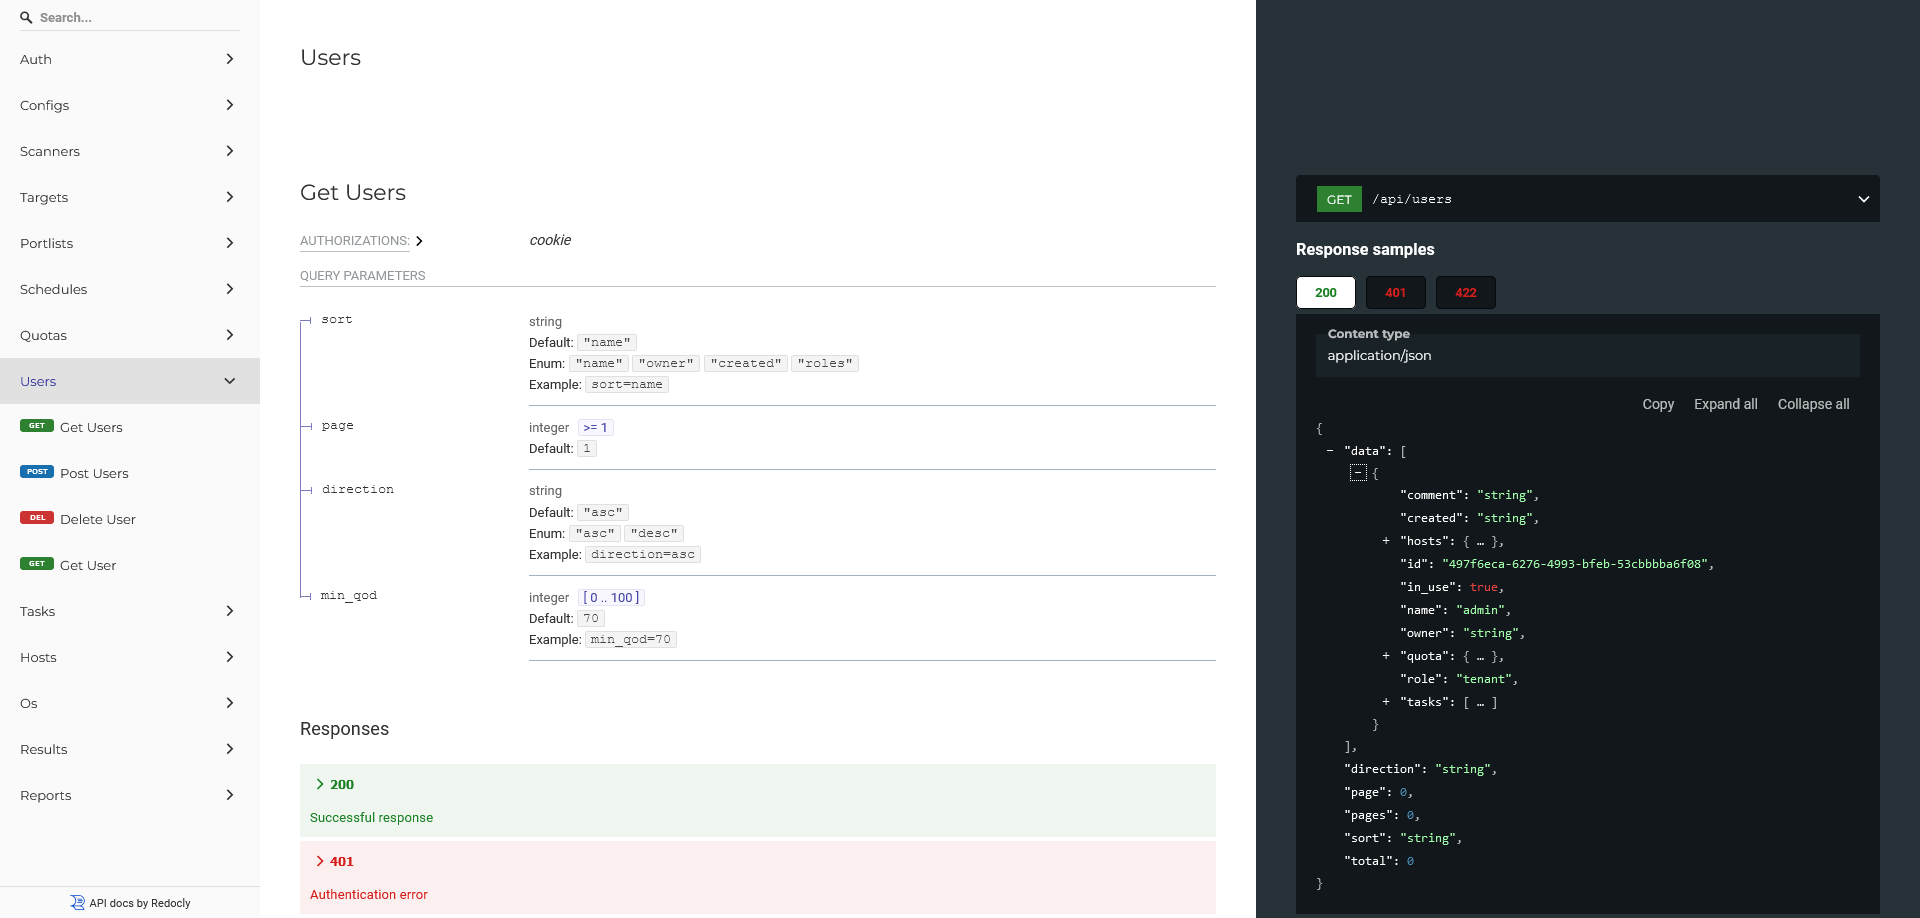
\includegraphics[width=\textwidth]{img/redoc.png}
\caption{Documentazione Redoc generata automaticamente da APIFlask}
\end{figure}
  \chapter{Sviluppo: Frontend}
  In cui si spiega nei dettagli lo sviluppo del frontend web facente veci di SPA.

\section{Client API}
Per questo componente un pezzo chiave è il client API. Nuxt offre diversi pattern, architetture e librerie per lo scopo.

\subsection{Prefisso}
Il file di configurazione di Nuxt (\texttt{nuxt.config.ts} \cite{nuxt-config}) consente di definire delle variabili e dei valori che vengono esposti all'intera applicazione.
Questi valori possono essere sovrascritti sulla base dei singoli ambienti (di sviluppo o produzione) mediante file \texttt{.env} appositi, rispettando lo standard DotEnv.
In questo modo è possibile definire e personalizzare flessibilmente il prefisso del server che ospita ed espone l'API, senza fissarlo nella \emph{codebase} e rendendolo al contempo facilmente disponibile all'ambiente JavaScript nel browser.

\subsection{Client Fetch}
Nuxt offre tre diverse modalità per l'ottenimento dei dati remoti, tutti basati sulla libreria \texttt{ofetch} \cite{ofetch}.

Queste diverse tecniche si rendono necessarie a causa della natura del framework Nuxt, che di fatto viene eseguito sia su client che su server. Come conseguenza di ciò, Nuxt esegue di fatto codice JavaScript isomorfo / universale su entrambe le parti. Perciò, richiedere i dati ``semplicemente'', senza ulteriori accorgimenti, darebbe vita a una doppia richiesta, una sul server (per creare l'HTML) e una sul client (quando l'HTML è idratato dal framework Vue). Questo può dare vita a tutta una serie di problemi, ma soprattutto:
\begin{itemize}
    \item \textbf{Hydration mismatch}: questo solitamente accade quando le risposte delle due richieste sono differenti, dando vita a un effetto visivo spiacevole in cui la pagina che si vede dal server ha contenuti basati sulla prima risposta, ma in un secondo momento (quando tutto il bundle JavaScript si è caricato) vengono sostituiti da quelli basati sulla seconda risposta.
    \item \textbf{Performance}: ovviamente, effettuare due volte una stessa richiesta aggiunge inutilmente ritardo ai tempi di caricamento.
\end{itemize}

Per risolvere questi problemi Nuxt include tecniche ulteriori che gestiscono automaticamente questa particolare situazione di richiesta dati, che in una SPA è una delle attività più frequenti e critiche:
\begin{itemize}
    \item \textbf{\texttt{\$fetch(...)}}: si tratta di un semplice alias per la libreria \texttt{ofetch}. Di fatto la funzione agisce come una classica e moderna libreria client HTTP, come ad esempio Axios. Non ha particolari strutture o organizzazioni per Nuxt, di conseguenza è in teoria riservata solo per le interazioni asincrone a pagina caricata (ad esempio: codice eseguito alla pressione di un bottone, chiedere dati all'apertura di un modale, \emph{polling} di dati a intervalli prestabiliti, ecc.)
    \item \textbf{\texttt{useFetch(...)}}: si tratta di un \emph{composable} per standardizzare le richieste di dati fatte nella funzione di \texttt{setup}, costruito a partire da \texttt{useAsyncData} e \texttt{\$fetch}.
    \item \textbf{\texttt{useAsyncData(...)}}: si tratta di un altro \emph{composable} che è responsabile per eseguire qualunque tipo di logica asincrona, non solo di richiesta dati da un server. Di fatto \texttt{useFetch} è un caso specifico di \texttt{useAsyncData}, cioè quello più comune, e fornisce semplice zucchero sintattico per questo scopo.
\end{itemize}

Nel nostro caso particolare la libreria di fetch di fatto si interfaccerà sempre e solo con un'API, di conseguenza ha senso cercare un modo di evitare inutili ripetizioni dell'URL del backend, centralizzandone la definizione. Il modo più facile ed elegante è utilizzare le funzionalità dedicate di \texttt{ofetch} per creare un ulteriore client che include tutte le opzioni specifiche per l'API, evitando di doverle specificare ogni volta.

Il client così creato dovrà essere reso disponibile in ogni parte del codice. Di conseguenza, la definizione del nuovo client è fatta in un \emph{plugin} Nuxt, ovvero un file TypeScript che definisce codice esposto dovunque nell'applicazione attraverso l'istanza di Nuxt.

\subsection{Token CSRF}
Come anticipato, si è introdotto un ulteriore livello di protezione mediante token CSRF, che deve essere recuperato al momento del caricamento della pagina e quindi incluso per ogni richiesta del client.

In pratica questo avviene facendo una richiesta nel \emph{plugin} definito come sopra. Questo si traduce in una chiamata singola fatta al momento del caricamento della pagina web, quando il bundle di codice JavaScript è caricato per la prima e unica volta. La richiesta va a toccare un endpoint specifico dell'API REST che restituisce il token CSRF sia come corpo che come header. Il token è quindi recuperato e incluso in ogni richiesta seguente semplicemente ponendolo come ulteriore pre-impostazione del client personalizzato per l'API GVM.

% solarized-light/dark, colorful, autumn, borland, emacs, pastie, tango, trac, vs
\begin{figure}
\centering
\begin{jscode}
export default defineNuxtPlugin(async (nuxtApp) => {
  const runtimeConfig = useRuntimeConfig()
  const {start, finish} = useLoadingIndicator()

  const response = await $fetch.raw(runtimeConfig.public.apiBaseUrl + '/api/csrf-cookie', {credentials: 'include'})
  const csrf_token = response.headers.get('X-CSRFToken')

  const api = $fetch.create({
    baseURL: runtimeConfig.public.apiBaseUrl + '/api',
    onRequest({ options }) {
      options.headers.set('X-Requested-With', 'XMLHttpRequest')
      options.headers.set('Content-Type', 'application/json')
      options.headers.set('Accept', 'application/json')
      if (csrf_token) {
        options.headers.set('X-CSRFToken', csrf_token)
      }
      options.credentials = 'include'
      start() // Inizia l'animazione della barra di caricamento
    },
    async onResponseError({ response }) {
      if ([401, 419].includes(response.status) && !response.url.endsWith('/api/login') && !response.url.endsWith('/api/logout') && !response.url.endsWith('/api/me')) {
        const {logout} = useAuth()
        logout()
        await nuxtApp.runWithContext(() => navigateTo('/login'))
      }
    },
    onResponse() {
      finish() // Conclude l'animazione della barra di caricamento
    }
  })

  return {
    provide: {
      api
    }
  }
})
\end{jscode}
\caption{Plugin Nuxt per il client API}
\end{figure}

\subsection{Componente Suspense}
Nuxt internamente usa il componente \texttt{<Suspense>} di Vue per ritardare la navigazione fino a che ogni richiesta asincrona non sia completata, evitando la resa bizzarra e improvvisa dei dati.

Questa funzionalità è di per sé attivata, ma può essere disattivata a seconda delle esigenze e anche su specifiche rotte di navigazione. Nel caso in esame si è preferito tenere attiva la funzionalità, non essendoci richieste troppo lente.

\subsection{Barra di caricamento}
In aggiunta, Nuxt fornisce un componente che renderizza automaticamente una barra di caricamento per il cambio vista e le navigazioni tra pagine, intercettando le richieste fatte con le proprie librerie.

Siccome il client in questo progetto è creato da zero usando direttamente \texttt{ofetch} allora segue che è necessario reintrodurre questo comportamento, agganciandosi ai \emph{callback} esposti dall'istanza \texttt{ofetch}. Nuxt offre anche un composable \texttt{useLoadingIndicator}, di fatto usato per fornire la barra di caricamento in modalità \emph{headless}. Nel nostro caso ci limiteremo a usarlo per governare la barra di caricamento sulla base dello stato delle richieste (semplicemente si avvia e termina assieme alla richiesta).

\section{Modalità di rendering}
Normalmente una SPA come quelle generate con framework client-side come Vue, React o Angular sul browser è caricata partendo dalla singola pagina HTML e quindi caricando l'insieme del codice JavaScript.

Come già discusso, questa modalità di caricamento presenta due principali problemi, ovvero la scarsa predisposizione all'indicizzazione da parte dei motori di ricerca (trascurabile nel nostro caso) e il rischio di lentezza durante il primo caricamento dell'applicazione web.

Per mitigare i precedenti due problemi Nuxt offre anche due diverse modalità di rendering alternative aggiuntive oltre a quella classica delle SPA:
\begin{itemize}
    \item \textbf{Server Side Rendering (SSR)}: in questo caso un componente server in JavaScript renderizza parte del contenuto web sul server a \emph{runtime} e al client ritorna la pagina web già parzialmente renderizzata, da completare in client-side.
    \item \textbf{Static Site Generation (SSG)}: in questo altro caso invece Nuxt genera a \emph{compile-time} le pagine statiche, che poi un semplicissimo web server ritorna all'utente.
\end{itemize}

Nel nostro caso si è deciso per una soluzione di SSR, siccome SSG chiaramente non può supportare le rotte dinamiche (cioè, ad esempio, URL che contengono l'UUID di una risorsa, perché chiaramente questi non possono essere determinati a \emph{compile-time} dal crawler di Nuxt).

\section{Autenticazione}
Come detto precedentemente, l'autenticazione è gestita mediante cookie di sessione, ma ci sono comunque alcuni accorgimenti architetturali di cui tenere conto.

\subsection{Composable di autenticazione}
La parte di autenticazione è particolarmente delicata e non banale da realizzare nel caso di una SPA, di conseguenza si è deciso per la creazione di un \emph{composable} dedicato allo scopo, chiamato \texttt{useAuth}.

Il componente espone di fatto tre funzionalità: tentare il login con delle credenziali date, effettuare il logout, recuperare l'utente attualmente connesso.

Questo composable è sfruttato anche nel client dell'API: se una qualunque richiesta ritorna uno stato interpretabile come un utente non autenticato nel sistema, cioè un codice 401, allora il client pulisce la sessione con un logout e ritorna alla schermata di login, di fatto rendendo il client reattivo ad eventuali cambiamenti improvvisi nel client o nel server.

\subsection{Middleware}
Nuxt consente anche di definire facilmente dei \textbf{middleware}, ovvero del codice JavaScript che è eseguito a discrezione del programmatore durante il passaggio tra una pagina e all'altra.

In questo progetto è stato realizzato un middleware che impedisce all'utente di andare su rotte non consentite o non pensate per il suo stato di autenticazione (un utente autenticato non può andare alla schermata di login e uno non autenticato non può andare dove il login non è concesso, cioè ogni altra rotta dell'applicazione).

\begin{figure}
  \centering
  \begin{jscode}
export default defineNuxtRouteMiddleware(async (to, from) => {
  const {user, initUser} = useAuth()
  await initUser()
    
  if (to.path !== '/login' && !user.value)
    return navigateTo('/login')
    
  if (to.path === '/login' && user.value)
    return navigateTo('/')
})
  \end{jscode}
  \caption{Middleware usato per controllare lo stato d'autenticazione}
\end{figure}

L'unione del middleware e del logout automatico fatto dal composable di fatto garantisce di reagire il prima possibile al logout dell'utente.

\section{Pagine e layout}
Nuxt dispone di un proprio sistema di \emph{templating} per le pagine web. Qui segue come si è strutturata l'applicazione all'interno di queste funzionalità.

\subsection{Layout}
I file di layout sono utilizzati per definire lo scheletro comune a tutte le pagine web dell'applicazione o a un loro sottoinsieme. In questa applicazione, di fatto una dashboard, si è fatto uso di due layout:
\begin{itemize}
    \item Un layout generico applicato a tutte le pagine web.
    \item Uno specifico per la pagina di login e solo per quella.
\end{itemize}
Da questa organizzazione si deduce facilmente che in buona sostanza l'intera applicazione può essere consultata / usata solo se precedentemente autenticati.

\begin{figure}
\centering
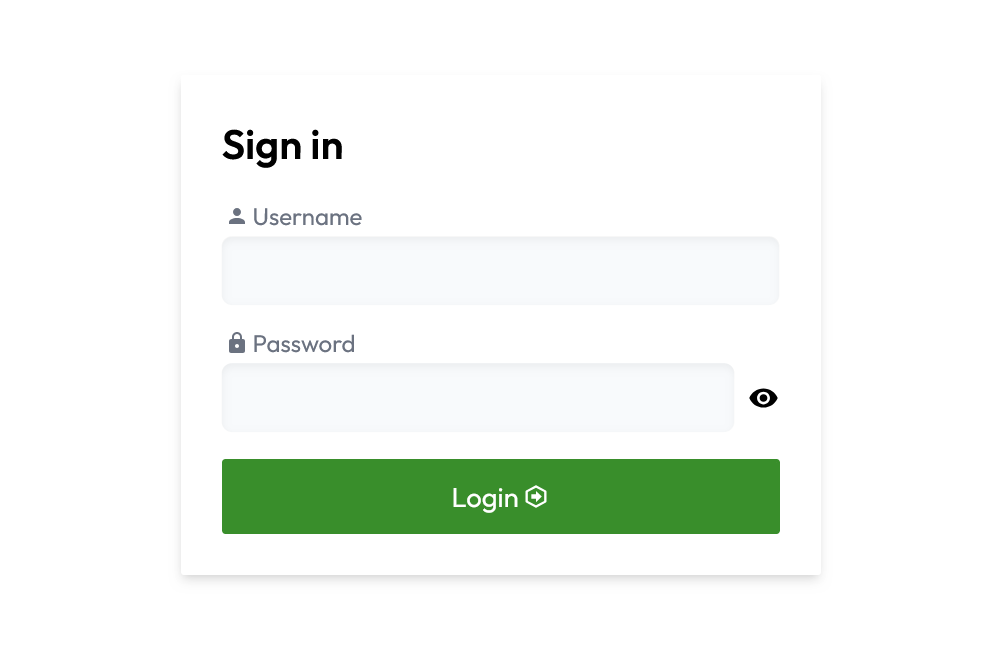
\includegraphics[width=0.8\textwidth]{img/login.png}
\caption{Layout / pagina di login}
\end{figure}

\subsection{Pagine}
Le singole pagine sono invece strutturate secondo il \emph{file-based routing} di Nuxt. In particolare, queste sono le principali pagine / rotte previste:
\begin{itemize}
    \item Login dell'utente.
    \item Homepage della dashboard, di fatto spoglia e priva di funzionalità particolari.
    \item Vista degli utenti. Nascosta a chiunque non abbia facoltà di gestione degli utenti. Permette di gestire utenti (cancellare, creare, ecc.)
    \item Vista delle task di scansione. Permette di creare task, verificare il progresso e l'esecuzione di quelli già configurati.
    \item Vista dei bersagli, da cui si possono vedere quelli già configurati e configurarne di nuovi.
    \item Viste dei risultati. Ne esistono di differenti per distinguere tra vulnerabilità vere e proprie e quelle ottenute tramite scansioni di prognosi \ref{cve}. Le viste integrano un sistema di filtraggio più avanzato e integrato rispetto alle altre strutture tabellari, siccome si presume che questa vista sarà quella su cui l'utente vorrà fare maggiori analisi.
    \item Viste dei rapporti. Di fatto fornisce un consuntivo dei risultati trovati e fornisce collegamenti ai risultati correlati e agli host determinati dalla scansione.
    \item Vista degli host. Raccoglie e visualizza degli host, con tutti i dettagli trovati organizzati nel modo più chiaro possibile.
\end{itemize}

\section{Store per QoD}
Come già detto, OpenVAS integra una stima empirica dell'affidabilità dei risultati raccolti, detta QoD. L'API realizzata espone questo parametro nelle richieste e fornendolo i risultati vengono automaticamente filtrati e restituiti solo quelli con QoD superiore al numero fornito.

Nell'interfaccia web si è deciso per avere un selettore di QoD globale, attivabile in ogni momento e la cui modifica influisce i risultati mostrati nelle pagine web. Questo si è realizzato nel concreto mediante un input range HTML, il cui valore è stato collegato tramite v-model ad una variabile di uno store Pinia.

Lo store Pinia consente di bypassare la struttura gerarchica dei componenti e di condividere globalmente la variabile del QoD ad ogni componente che ne ha bisogno.

\begin{figure}
\centering
\begin{jscode}
import { defineStore } from 'pinia'

export const useQoDStore = defineStore('qod', {
  state: () => ({ min_qod: 70, disable_input: false }),
  actions: {
    updateQoD(qod: number) {
      this.disable_input = true
      this.min_qod = qod
    },
    enableInput() {
      this.disable_input = false
    }
  }
})
\end{jscode}
\caption{Store Pinia usato per la condivisione del valore di QoD nel frontend}
\end{figure}

\section{Tipi TypeScript}
Nuxt è un framework profondamente radicato in TypeScript, per fornire type safety e altri controlli.

I tipi sono definiti in file \texttt{.d.ts}, in accordo con le convenzioni TypeScript. Di fatto sono quasi tutte interfacce TypeScript che replicano la struttura dei tipi già specificata negli schemi Marshmallow del backend.

\section{Componenti Vue}
Nuxt memorizza i componenti in una cartella \texttt{components/} gestita secondo convenzioni. In particolare, il nome delle cartelle induce automaticamente la struttura usata per effettuare import automatici dei componenti all'interno delle pagine, dei layout e di tutti gli altri componenti Vue.

Segue una spiegazione dei componenti più importanti e/o peculiari.

\subsection{Tabelle}
I componenti più importanti sono sicuramente le tabelle che organizzano e mostrano le entità. E fra questi, quello più importante è il componente generico su cui tutte le altre si basano.

\begin{figure}
\centering
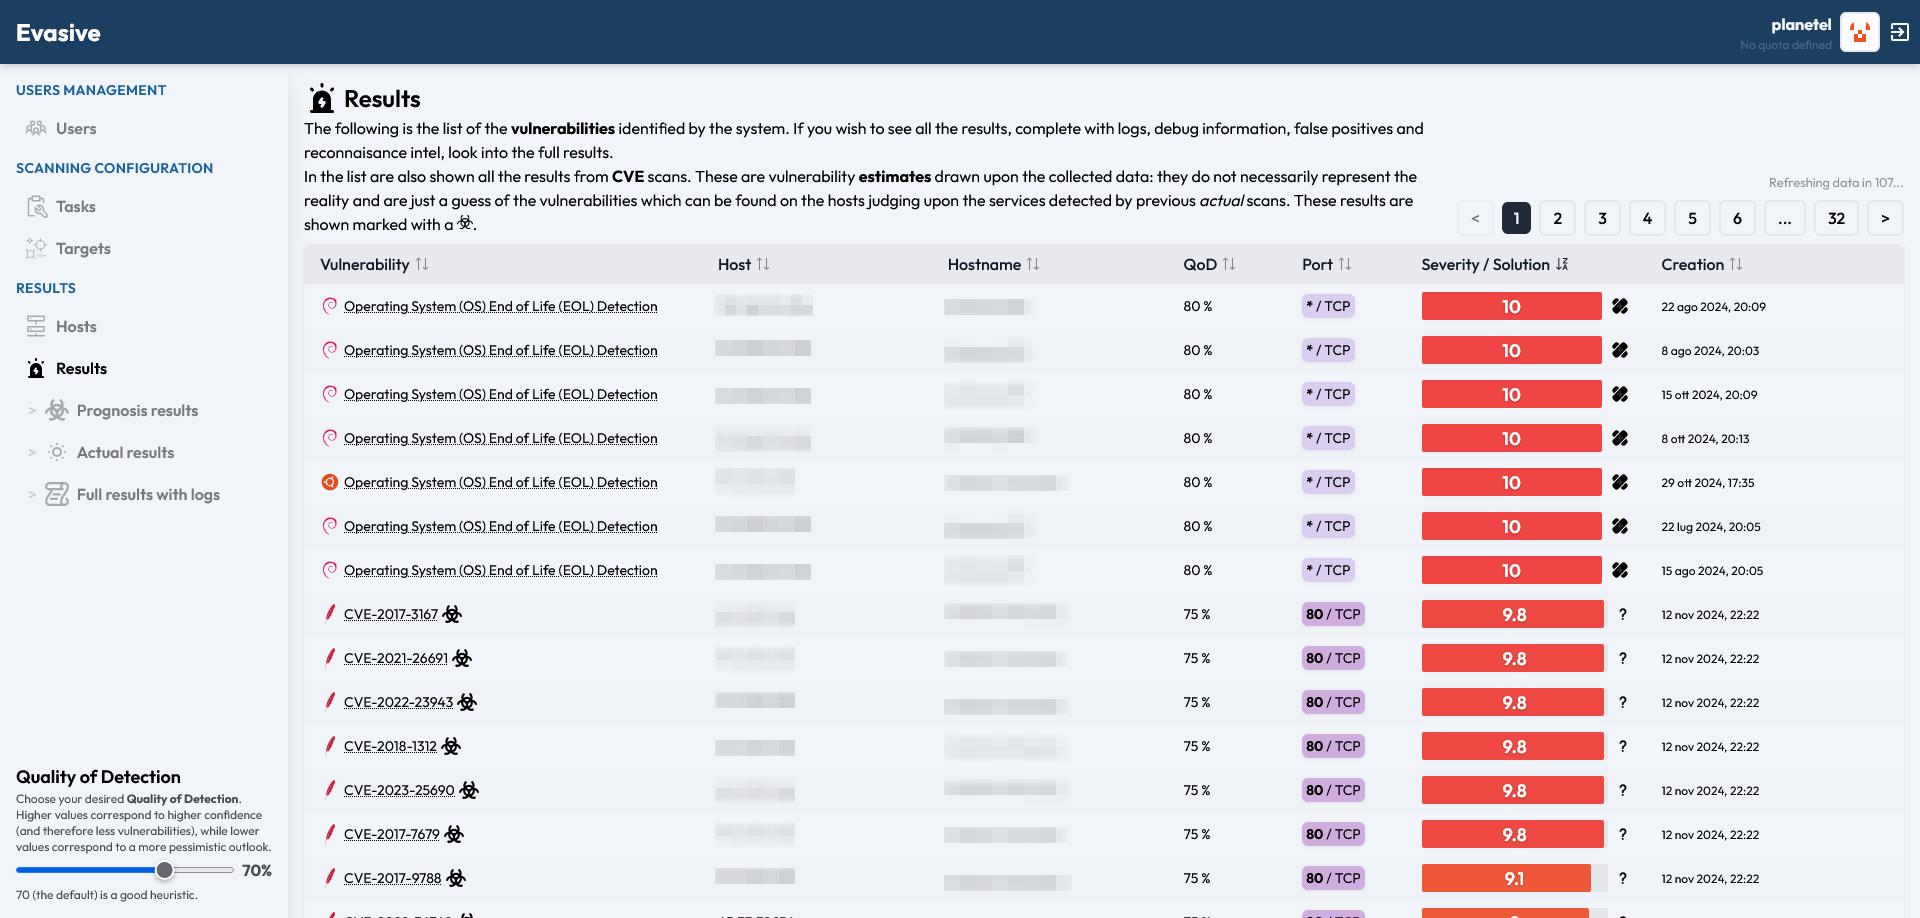
\includegraphics[width=\textwidth]{img/results.png}
\caption{Tabella dei risultati ottenuti dalle scansioni}
\end{figure}

\subsubsection{Razionale}
Di fatto il componente generico agisce come una sorta di tabella \emph{headless} che può essere configurata a seconda del caso specifico.

In questo modo si è riusciti ad avere una sorta di griglia dei dati similare come concetto a quelle fornite da librerie come Ag-Grid. Tuttavia, l'aver realizzato questo componente in autonomia consente di applicare uno stile d'aspetto specifico per il nostro progetto.

Questo comportamento è molto simile a quello che offrono librerie come Tanstack \cite{tanstack}, che forniscono componenti headless. Tuttavia, dopo un'attenta valutazione si è giunti alla conclusione che integrare librerie così avanzate sarebbe stato troppo lavoro per funzionalità aggiuntive che non si sarebbero mai usate. Inoltre, questo ha consentito di creare un'interfaccia più adatta e specifica per i nostri scopi.

\subsubsection{Funzionalità}
Il componente così creato offre le seguenti funzionalità:
\begin{itemize}
    \item Titolo, icona e altre opzioni di aspetto e contenuto sono completamente personalizzabili dagli attributi.
    \item Descrizione e azioni della tabella sono configurabili tramite \emph{named slot}. Le azioni di ogni riga sono configurabili tramite \emph{scoped slot}.
    \item Personalizzazione e scelta dell'entità che gestisce attraverso l'inserimento dell'endpoint responsabile di fornire le entità. Questo può funzionare siccome la REST API agisce in modo standardizzato per tutte le richieste indice.
    \item Reagisce ai campi di QoD.
    \item Supporta e gestisce autonomamente una paginazione di tipo server-side usando i dati forniti dal backend.
    \item Supporta il filtraggio dei dati, se dichiarato possibile dall'interfaccia.
    \item Supporta l'ordinamento \emph{server-side} delle colonne, se dichiarato possibile dalle definizioni delle colonne.
    \item \emph{Polling} dei dati ad intervalli regolari, realizzando l'aggiornamento dinamico dello stato delle scansioni, dei rapporti e dei risultati. Per questa parte è stato necessario ricorrere a \textbf{VueUse} una libreria popolare di Vue 3, che fornisce dei \emph{composable} snelli e leggeri per facilitare l'integrazione delle funzioni standard nel nuovo paradigma di Vue.
    \item Il componente gestisce in autonomia accorgimenti al frontend per gestire elegantemente gli stati di caricamento.
    \item Le righe della tabella sono animate con il componente TransitionGroup di Vue.
    \item Può mostrare un bottone il cui evento apre un modale. Il modale ha contenuto personalizzabile attraverso un Component Vue.
\end{itemize}

\subsubsection{Realizzazione}
Per realizzare il componente si sono usate varie feature di Vue e eventuali librerie aggiuntive.

La maggior parte delle opzioni del componente sono specificabili usando il meccanismo degli attributi / props, soprattutto booleani e stringhe, ma in alcuni casi anche oggetti JavaScript più strutturati:
\begin{itemize}
    \item Il componente incluso nel modale apribile dall'apposito bottone di aggiunta è specificabile tramite un Component. Siccome Nuxt usa un meccanismo di import automatico è necessario importare manualmente il componente, usando la macro \texttt{\#components} messa a disposizione da Nuxt apposta per queste situazioni.
    \item Le definizioni delle colonne, che specificano le proprietà di ognuna di essa: quale campo considerare nell'oggetto fornito, che tipo di dato è, quale \emph{renderer} usare per mostrare il dato, se la colonna è ordinabile, filtrabile e altre personalizzazioni di stile. Questo approccio è abbastanza simile a quello utilizzato da Tanstack \cite{tanstack}, sebbene più semplice e diretto.
\end{itemize}

Nel componente si è anche usata una feature di Vue abbastanza recente (3.3) ovvero i \textbf{componenti generici}. Questa funzionalità consente di definire e usare tipi generici nella funzione di \texttt{setup} del componente. Nel caso specifico si è definito un tipo generico per l'entità considerata dalla tabella.

\subsection{Renderer}
I \emph{renderer} altro non sono che un insieme di componenti dedicati a prendere un dato semplice (una stringa di caratteri, un booleano, un intero, un decimale) o strutturato (un oggetto JSON o un'array di oggetti o variabili) per poi mostrarlo all'utente in una forma \emph{user-friendly} e stilisticamente accattivante.

Nel progetto ci sono quasi 40 renderer differenti e/o innestati l'uno nell'altro, di fatto diventando una sorta di ``design pattern'' di progetto. L'uso di questo sistema porta diversi benefici:
\begin{itemize}
    \item Siccome il progetto usa un framework CSS \emph{utility-first} il segregare lo stile il più possibile in componenti atomici garantisce manutenibilità e riproducibilità.
    \item Similarmente, tanti componenti granulari garantiscono un facile riuso e quindi facile manutenibilità e ridondanza ridotta al minimo.
    \item Renderizzare anche il dato ``semplicemente'' senza ulteriori personalizzazioni fornisce un comodo livello di indirezione per aggiungere ulteriori personalizzazioni in futuro.
    \item Inoltre, renderizzare i dati in questo modo consente di realizzare personalizzazioni più avanzate che semplici modifiche stilistiche, permettendo di integrare del comportamento (apertura di modali, \emph{tooltip}, link a pagine web, ecc.)
\end{itemize}

\begin{figure}
\centering
\begin{vuesfc}
<script setup lang="ts">
import { DateTime } from 'luxon'
  
defineProps<{ value: string }>()
</script>
  
<template>
  <span v-if="value" class="text-xs truncate">
    {{ DateTime.fromISO(value).toLocaleString({month: 'short', day: 'numeric', year: 'numeric', hour: '2-digit', minute: '2-digit'}) }}
  </span>
  <span v-else />
</template>
\end{vuesfc}
\caption{Renderer usato per i timestamp, basato sulla libreria Luxon}
\end{figure}

\subsubsection{CPE}
Un renderer particolarmente interessante è quello usato per i CPE. OpenVAS infatti utilizza stringhe che rispettano il formato CPE per specificare gli \emph{asset} inventariati dalle scansioni (host e OS), ma anche l'ambiente in cui una vulnerabilità è stata rilevata.

Per rendere la consultazione dei risultati il più possibile veloce si è deciso di mostrare i CPE corredandoli di icone. Queste sono determinate a partire dai \emph{vendor} (o dai \emph{product}) specificati nella stringa CPE.

\begin{figure}
\centering
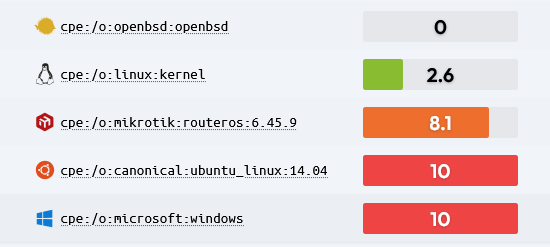
\includegraphics[width=0.6\textwidth]{img/cpe.png}
\caption{Renderer delle stringhe CPE e dei punteggi di severità}
\end{figure}

\subsubsection{Iconify}
Molti dei renderer sfruttano le icone SVG per facilitare la visualizzazione dei dati a colpo d'occhio.

Le icone sono fornite dalla libreria \textbf{Iconify} che porta in dote decine di migliaia di icone raccolte dai principali pacchetti disponibili online; queste sono poi richieste \emph{on demand} da un componente apposito (Iconify mette a disposizione un comodo wrapper per Vue).

\subsection{Modali}
I modali sono definiti tutti a partire da un componente comune, che ne fornisce le funzionalità di base. Il contenuto è personalizzabile con lo slot di default.

La caratteristica fondante di un modale è che questo in un certo senso esce dalla gerarchia del documento HTML. Questo è realizzato anche in pratica con il componente \texttt{Teleport} di Vue, che trasferisce il componente sotto il tag body.

L'apparizione del modale è animata con il componente \texttt{Transition}.

\subsection{Form}
Le form sono un altro pezzo essenziale dell'applicazione. Come in ogni progetto, la parte fondamentale e più critica di queste componenti riguarda l'inserimento e la validazione dei dati, che dev'essere il più possibile semplice e intuitivo.

\subsubsection{Validazione}
Per quanto riguarda la validazione ci si è integrati con \textbf{Vee-Validate} \cite{vee-validate}, una delle più popolari librerie di validazione \emph{client-side}. Trattandosi di validazione client-side si è badato soprattutto a fornire un \emph{feedback} veloce e informativo per l'utente. Infatti, tutti i dati sono comunque validati \emph{server-side} tramite gli schemi Marshmallow.

\subsubsection{Select e option}
Per rendere l'input dei dati il più facile possibile si è fatto largo uso del paradigma di input fornito dai tag HTML di select, ovvero i menu a discesa. In questo modo la validazione dei dati è semplificata, ma anche l'esperienza utente, che ha a disposizione un piccolo insieme di opzioni ben chiare tra cui scegliere.

Tuttavia, il componente nativo di select è piuttosto limitato:
\begin{itemize}
    \item Le opzioni permettono di avere solo testo semplice, con pochissime personalizzazioni consentite.
    \item Non esiste una possibilità di filtraggio.
\end{itemize}
Per ovviare a queste limitazioni si è fatto larghissimo uso di \texttt{vue-multiselect}, una comodissima libreria che fornisce un componente di selezione accessibile e molto personalizzabile, sia come aspetto che come comportamento.

Per ogni componente di selezione si è sfruttata questa libreria, realizzando inoltre dei componenti dedicati per il \emph{rendering} di ogni singola opzione. In questo modo, ogni componente di selezione è personalizzato appositamente per lo scopo, con icone e descrizioni, rendendo l'input dei dati particolarmente veloce e semplice.

\begin{figure}[!h]
\centering
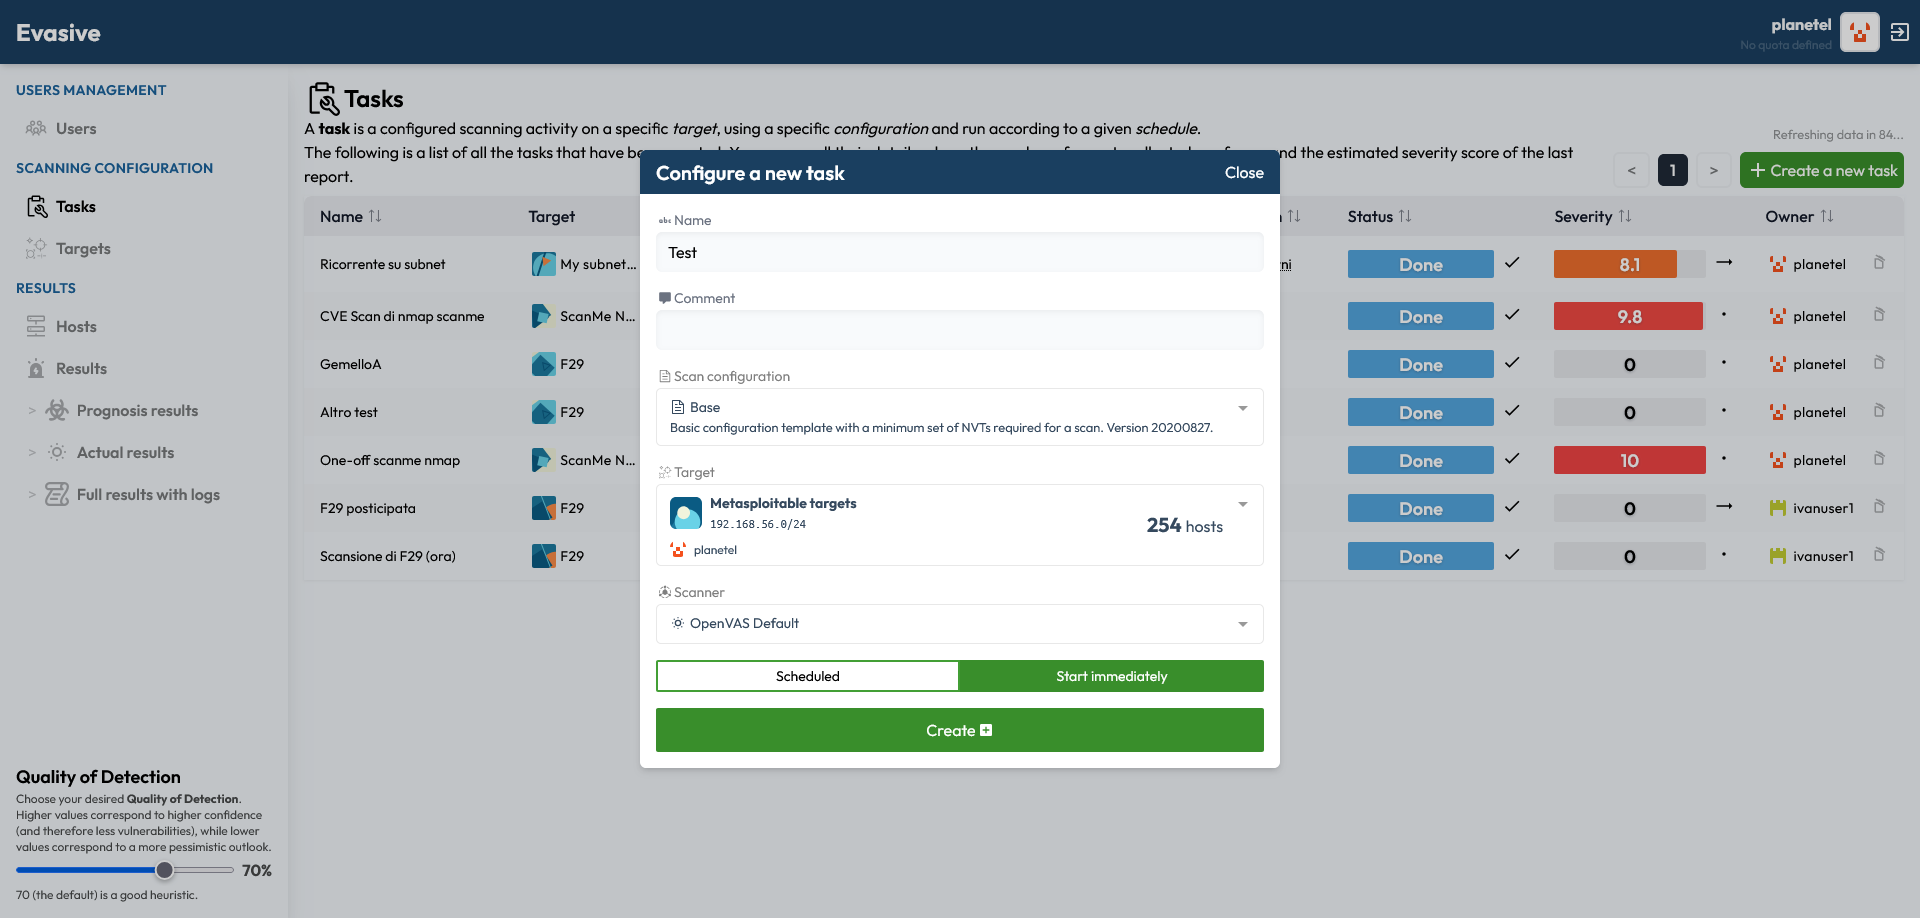
\includegraphics[width=\textwidth]{img/form-task-now.png}
\caption{Form per l'aggiunta di un nuovo task di scansione}
\end{figure}

\begin{figure}[b]
\begin{vuesfc}
<script setup lang="ts">
defineProps<{
  showModalIf: boolean;
  title: string;
}>()

defineEmits(['close'])
</script>

<template>
  <Teleport to="body">
    <Transition name="modal-fade">
      ...
    </Transition>
  </Teleport>
</template>

<style scoped>
.modal-fade-enter-from,
.modal-fade-leave-to {
  opacity: 0;
}
.modal-fade-enter-active,
.modal-fade-leave-active {
  transition: 0.25s ease all;
}
.modal-wrapper {
  position: fixed;
  left: 0;
  top: 0;
  z-index: 100;
  width: 100vw;
  height: 100vh;
  background: rgba(0, 0, 0, 0.2);
  display: grid;
  place-items: center;
}
</style>
\end{vuesfc}
\caption{Modale generico definito con i costrutti idiomatici di Vue}
\end{figure}
  \chapter{Deployment}
  In cui si spiega brevemente il processo di installazione del software su di un server di produzione.

\section{Struttura}
Il sistema così realizzato finora consta di due componenti:
\begin{itemize}
    \item \textbf{SPA / frontend applicativo}: interagisce con il backend tramite protocollo HTTP.
    \item \textbf{REST API / backend applicativo}: risponde alle richieste del frontend attraverso l'interfacciamento con la socket UNIX del sistema Greenbone.
\end{itemize}
Dall'ultimo punto segue che la REST API e l'istanza del sistema Greenbone devono trovarsi necessariamente sullo stesso server. In alternativa, almeno il demone GVM deve essere presente sullo stesso server.

La SPA di frontend tuttavia può trovarsi anche su di un server differente e interagire con l'API del backend Flask tramite protocollo HTTP. Questo può aprire interessanti possibilità di ottimizzazione se si vuole usare delle CDN o altri strumenti di edge computing.

Nel nostro caso specifico tuttavia entrambi i componenti sono stati installati sullo stesso server, per pura semplicità.

\section{Containerizzazione}
L'installazione delle componenti e la loro integrazione con il sistema Greenbone sono state entrambe realizzate attraverso Docker (e più nello specifico, Docker Compose).

Infatti, come già detto in \ref{greenbone-community-containers}, Greenbone mette a disposizione un'installazione ufficiale e supportata dell'intero framework attraverso la piattaforma di Docker Compose. Per un ambiente di produzione questa strategia garantisce riproducibilità e affidabilità, ma anche un aggiornamento in generale estremamente semplice, per il quale basta distruggere i container esistenti, aggiornare le immagini di Docker e ricreare i container.

Questo di fatto guida il processo di installazione verso una strategia semplice, ma efficace: \emph{dockerizzare} (ovvero realizzare un Dockerfile) entrambe le componenti realizzate per questo progetto (frontend e backend) e interconnetterle in Docker Compose tramite due container appositi.

\subsection{Immagine del backend}
\label{deployment-backend}
Il backend è stato trasposto in un container Docker secondo il seguente procedimento, seguendo a grandi linee il seguente \texttt{Dockerfile}:
\begin{figure}[!h]
    \centering
    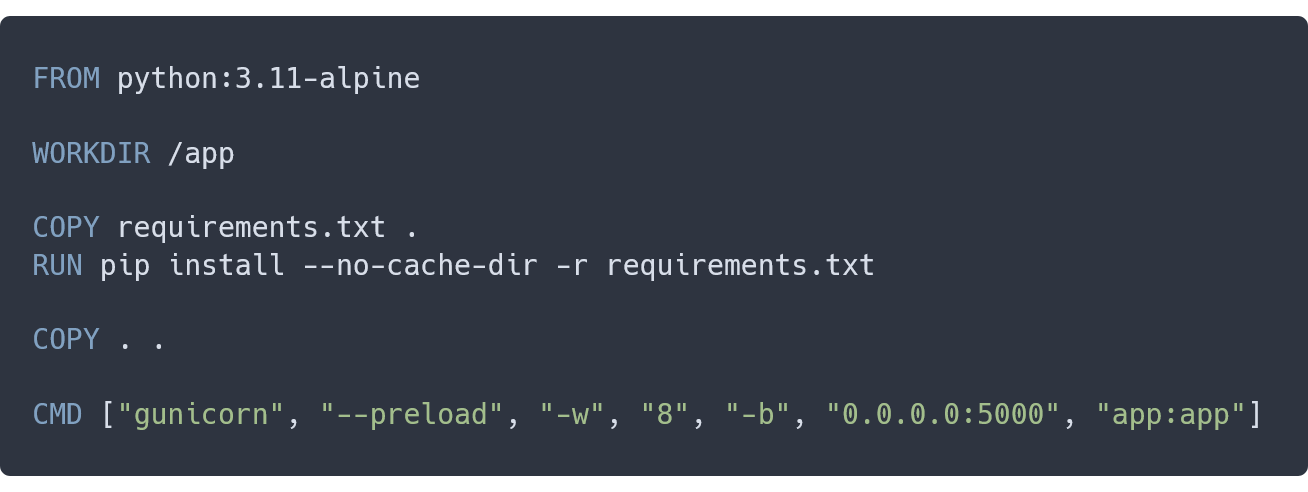
\includegraphics[width=0.8\textwidth]{img/dockerfile-backend.png}
    \caption{Dockerfile usato per l'immagine del backend Flask}
\end{figure}
\begin{enumerate}
    \item Si parte da un'immagine di base della versione di Python utilizzata durante lo sviluppo del progetto. La versione \texttt{alpine} garantisce un minor consumo di spazio di disco\footnote{Le immagini \texttt{alpine} si riferiscono a immagini Docker basate su \textbf{Alpine Linux}, una distribuzione Linux leggera e minimalista. Alpine è progettata per essere piccola, sicura e semplice, il che la rende una scelta popolare per la creazione di container Docker, dove il sistema operativo richiesto tipicamente deve eseguire non più di un'applicazione. Gran parte della riduzione di dimensioni è dovuta all'uso di \texttt{musl} come libreria C al posto della più famosa \texttt{glibc}. \texttt{musl} infatti è molto più piccola e coesa, ma c'è sempre il rischio che alcune applicazioni non funzionino come dovrebbero in un ambiente Alpine, siccome si aspettano la libreria \texttt{glibc} che ormai è uno standard di fatto in ambiente Linux.}.
    \item Nell'immagine viene copiato solo il file delle dipendenze (\texttt{requirements.txt}), che vengono installate con \texttt{pip}. In questo modo si può sfruttare al massimo il \emph{caching} dei layer di Docker.
    \item Il codice viene copiato nella sua totalità.

    In questo passaggio viene anche copiato nell'immagine il file \texttt{.env}, che chiaramente deve essere creato e configurato non essendo stato aggiunto al sistema di controllo versione.

    In particolare, il file dovrebbe essere configurato con:
    \begin{itemize}
        \item Una chiave di crittografia, necessaria siccome usiamo i cookie di Flask. Questa può essere creata facilmente e in sicurezza usando un interprete di Python per generarla in modo crittograficamente sicuro.
        \item Il numero massimo di IP configurabili per ogni bersaglio in GVM.
        
        Di default un'installazione del framework Greenbone è configurata con un massimo di $2^{12}-1$ IP per bersaglio, ma questa soglia può essere alzata in un secondo momento sino ad un limite di $\approx 70000$ che essendo $> 2^{16}$ permette almeno di configurare anche subnet $/16$ in notazione CIDR, che sono comuni in molti contesti aziendali.
        \item Gli UUID dei ruoli configurati come da schema descritto in \ref{roles}. Questi possono essere facilmente ottenuti tramite GSA.
        \item IP, porta, DB e password dell'istanza Redis. Siccome stiamo usando Docker Compose l'istanza di Redis di fatto è ospitata su un container dedicato, quindi la porta sarà quella usata dal container (che può essere tranquillamente quella di default senza problemi di sicurezza, visto che non sarà pubblicata al di fuori della macchina) mentre l'IP è il nome dato al container che nelle funzionalità di rete offerte da Docker funge da hostname.
    \end{itemize}
    \item Come entrypoint si utilizza il web server WSGI\footnote{\textbf{Web Server Gateway Interface} è un'interfaccia standard tra web server e applicazioni web scritte in Python. Molti dei più famosi framework Python come Flask e Django aderiscono allo standard WSGI, e pertanto possono essere facilmente installati grazie a web server anch'essi compatibili con WSGI. Gunicorn è uno dei più famosi server web di questo tipo, e può essere installato come una semplice dipendenza \texttt{pip}.} \textbf{Gunicorn}, configurato per precaricare il codice precedentemente al fork dei processi worker.
\end{enumerate}

\subsection{Immagine del frontend}
Il frontend invece segue il seguente \texttt{Dockerfile}:
\begin{figure}[!h]
    \centering
    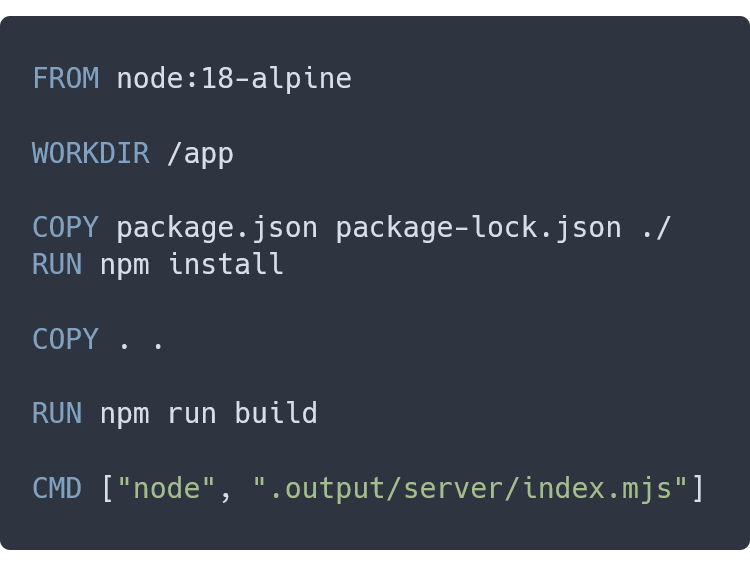
\includegraphics[width=0.5\textwidth]{img/dockerfile-frontend.png}
    \caption{Dockerfile usato per l'immagine del frontend Nuxt}
\end{figure}
\begin{enumerate}
    \item Come immagine di base si è scelta una \texttt{node} della versione corrispondente a quella usata nell'ambiente di sviluppo.
    \item Nell'immagine vengono copiati i file \texttt{package.json} e \texttt{package.lock}, per poi installare le dipendenze con \texttt{npm}.
    \item Viene copiato il resto del codice. Anche qua viene fatto questo passaggio ulteriore per sfruttare il \emph{caching} delle immagini Docker. Inoltre, viene copiato il file \texttt{.env}, che deve essere creato e configurato con l'unica variabile rilevante: l'endpoint dell'API. Si noti che in questo caso è necessario fornire un endpoint visibile dal web, siccome questo indirizzo sarà usato per le richieste fatte dal client Fetch di Nuxt, che non funzionano in ambiente Docker (e pertanto inserire l'hostname del container di Flask non funzionerebbe).
    \item Tramite \texttt{nuxt build} si crea il componente server usato da Nuxt per la SSR, basato su Node e Nitro. Questo componente viene prodotto sotto \texttt{.output/server/index.mjs}.
    \item Come entrypoint si richiama il componente server creato al punto precedente con l'interprete Node.
\end{enumerate}

\subsection{Redis}
Il backend Flask necessita di un'istanza di Redis per la gestione delle sessioni server-side. Questa può essere creata facilmente con l'immagine Redis disponibile su Docker Hub.

\subsection{Nginx}
L'accesso ai due componenti realizzati è mediato dal web server Nginx, che fa da \emph{reverse proxy} nei confronti degli altri container:
\begin{itemize}
    \item Tutte le richieste a \texttt{/api} sono rimandate al container Flask, usando il suo hostname e la sua porta.
    \item Tutte le altre richieste sono demandate al container del frontend.
\end{itemize}
Il web server Nginx è una delle uniche porte esposte al di fuori del server, usando quelle standard del protocollo HTTP / HTTPS.

\label{cors-deployment}
Si noti come in produzione il CORS non sia necessario, siccome API e server web sono esposti sulla stessa origine grazie ad Nginx.

\subsection{Interconnessione in Docker Compose}
\label{compose-architecture}
Tutto questo è assemblato nell'architettura illustrata in figura \ref{fig:architecture}:
\begin{itemize}
    \item Il reverse proxy Nginx media l'accesso al frontend alternativo a OpenVAS e al suo backend di interconnessione che controlla l'uso delle risorse e implementa la multi-tenancy, realizzando quindi i requisiti chiave del progetto.
    \item GSA rimane comunque esposto per avere un accesso senza filtri a GVM tramite l'interfaccia originale, utilizzabile da amministratori di sistema e sviluppatori.
    
    Si noti che è possibile implementare permessi agli utenti e ai ruoli per impedire l'accesso tramite GSA a utenti comuni, come ulteriore precauzione di sicurezza.
    \item Il volume della Socket UNIX gestito in Docker è l'anello di interconnessione fondamentale tra la parte di Docker Compose ``originale'' del progetto e quella iniziale proposta dal sistema GVM.
\end{itemize}
\begin{figure}
    \centering
    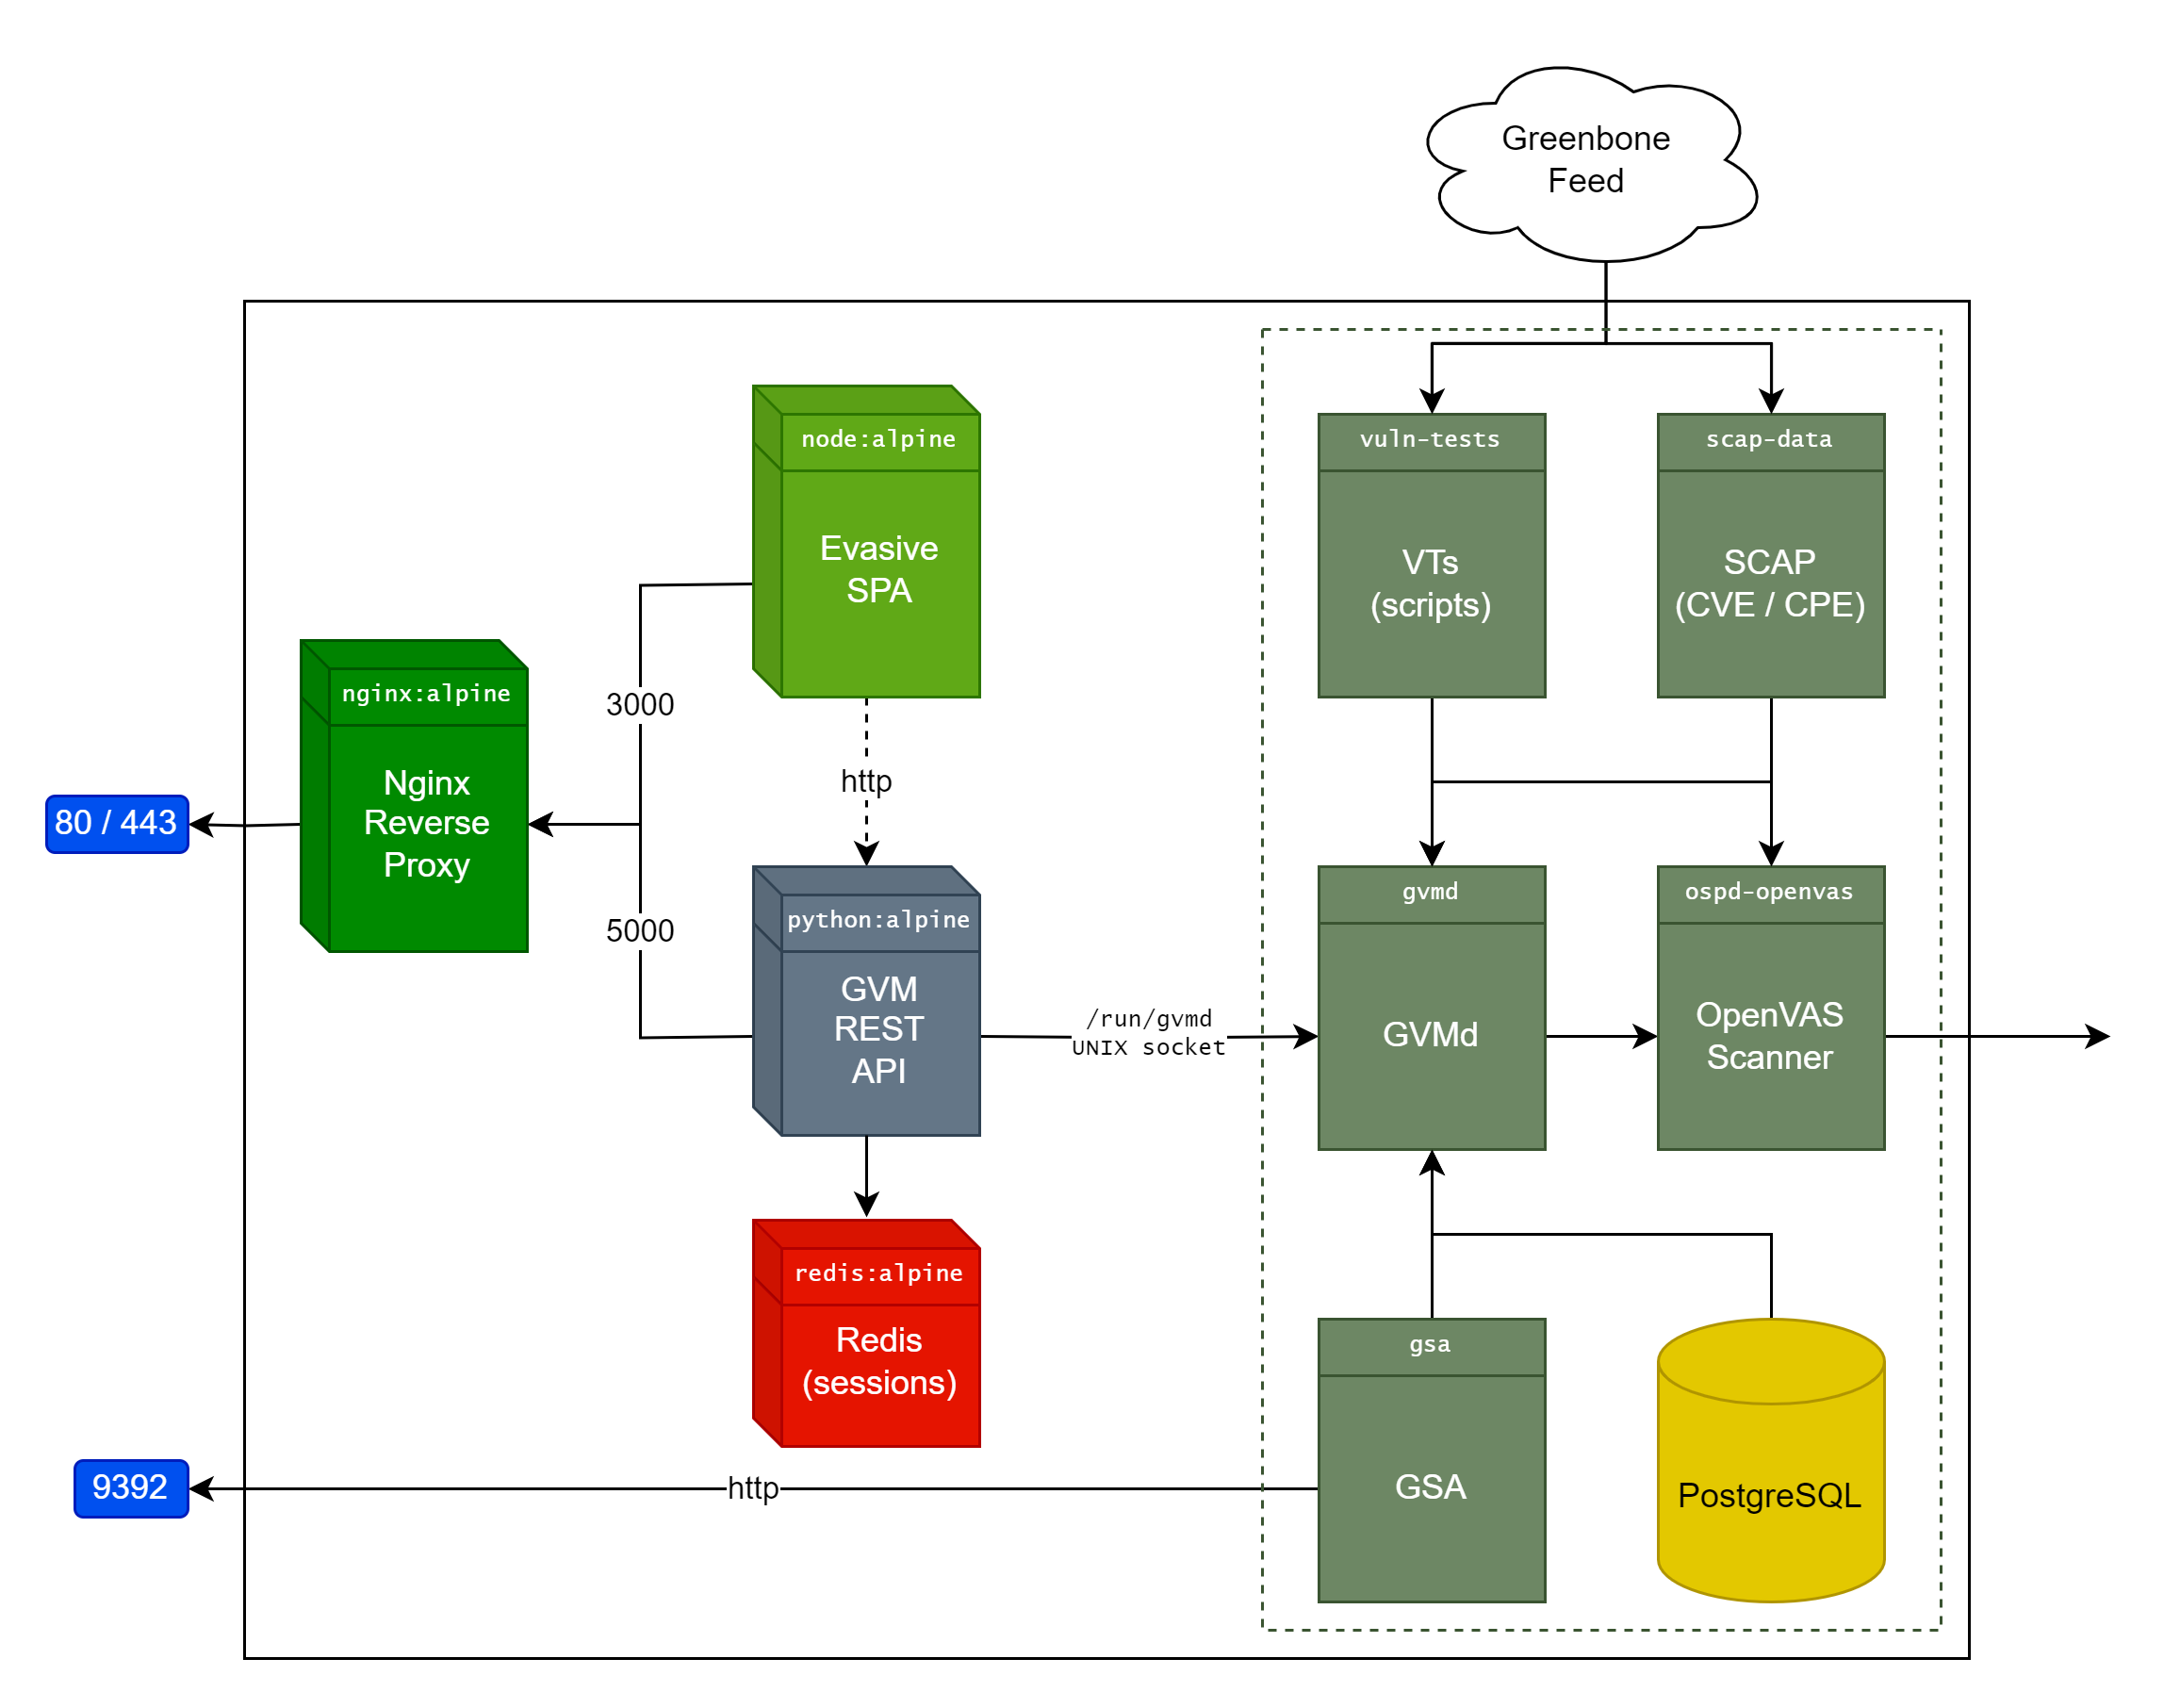
\includegraphics[width=\textwidth]{img/systems.png}
    \caption{Struttura generale dei container specificati con Docker Compose, nonché delle principali interconnessioni con il sistema Greenbone. Si noti che il framework Greenbone contiene molti più componenti di quelli elencati nel grafico, di cui molti utilizzati \emph{una tantum} dallo stesso framework. L'interconnessione centrale con il sistema Greenbone (tratteggiato) avviene mediante un volume Docker condiviso tra il container del demone GVM e il container del backend Flask. Sono presenti anche altri volumi Docker usati per la persistenza di altri dati in ambo le parti (es. le sessioni di Redis e PostgreSQL), ma non sono stati riportati nel diagramma per leggibilità.}
    \label{fig:architecture}
\end{figure}
  \chapter{Conclusione}
  Il progetto realizzato per questo lavoro è stato realizzato dietro richiesta specifica di un'azienda di telecomunicazioni, e con il supporto della stessa durante tutte le fasi dello sviluppo per quanto riguarda l'erogazione dell'infrastruttura di produzione e la specifica dei requisiti. Tutto il lavoro di progettazione, codifica e installazione è stato invece svolto in totale autonomia dall'autore di questo documento.

\section{Analisi del lavoro svolto}
L'azienda ha avuto modo di verificare l'efficacia del prodotto sviluppata in un collaudo. In questa occasione il prodotto realizzato è stato ritenuto valido già allo stato attuale e degno di commercializzazione, ma anche di futuri sviluppi più accorti.

Tra i principali punti di forza riscontrati rientrano:
\begin{itemize}
    \item L'interfaccia del frontend facilitata, moderna e accattivante rispetto a quella più grezza e spartana di GSA.
    \item La separazione dei compiti realizzata tramite l'architettura a microservizi, che facilita l'eventuale integrazione futura integrazione futura con scanner diversi da OpenVAS.
    \item La facilità d'uso e d'interpretazione dei risultati.
\end{itemize}

\section{Futuri sviluppi e miglioramenti}
Il lavoro ha chiaramente evidenziato numerosi punti di miglioramento essendo di fatto solamente un solido prototipo, limitato nelle funzionalità sin dalle fasi di progettazione.

Tra i principali punti di miglioramento rientra sicuramente la generalizzazione ulteriore del sistema. Infatti, nonostante la separazione dei compiti tramite i microservizi ci sono molte terminologie e agganci specifici con il sistema di OpenVAS (la QoD, i ruoli, i gruppi e i permessi). In generale, gran parte di questo accoppiamento indesiderato deriva dalla scelta semplificativa di volersi appoggiare al database di OpenVAS, evitando la complicazione di volersi creare un proprio DB e un proprio schema di dati. Questo come abbiamo visto ha portato ad un sistema funzionante ed anche efficace, ma poco flessibile nel caso in un futuro dovesse presentarsi l'esigenza o la convenienza a spostarsi ad un altro sistema di scansione.

Inoltre, disaccoppiarsi dal database di OpenVAS consentirebbe di gestire quote e volumi di scansione in modo più idiomatico e proprio rispetto al dover sfruttare i tag di OpenVAS per ricreare funzionalità non previste dal framework di Greenbone con \emph{escamotage} che a qualcuno potrebbero apparire come ``hack''.

Inoltre, i task creati al momento sono costretti a rispettare una schedule mensile, ma disaccoppiarsi dal database interno di Greenbone consentirebbe di pensare anche a schedule più diversificate e flessibili con maggior facilità.

Un ulteriore punto di miglioramento è la gerarchia degli utenti. Infatti, allo stato attuale non sono stati approntati utenti in grado di consultare semplicemente i risultati, un ruolo che nella pratica è comune in molti contesti aziendali (dove un'amministratore di rete crea i task di scansione e una figura dirigenziale può solo controllare i risultati).

  \printbibliography
\end{document}